\documentclass[phd,project]{ppgccufmg}    % ou [msc] para dissertações
                                  % de mestrado. Para propostas ou
                                  % projetos, usar [phd,project],
                                  % [msc,proposal], etc.

%\usepackage[brazil]{babel}        % se o documento for em português, OU
\usepackage[english]{babel}      % se o documento for em inglês
%\usepackage[latin1]{inputenc}
\usepackage{xcolor,colortbl}%johnatan configuração da tabela 
%\usepackage[caption=false]{subfig}
\usepackage{subfloat}
%\usepackage{subfigure}
\usepackage{rotating}%johnatan
\usepackage{comment}

\usepackage{natbib}
\usepackage{graphicx}
\usepackage{multirow}

\usepackage{subfigure}

%####### Simbolo de checked######################
\usepackage{bbding}
\usepackage{amssymb}
\usepackage{pifont}
\newcommand{\xmark}{\ding{55}}%
%###############################

\usepackage[utf8]{inputenc}
\usepackage[T1]{fontenc}
\usepackage{type1ec}
\usepackage{graphicx}
\usepackage[a4paper,
  portuguese,
  bookmarks=true,
  bookmarksnumbered=true,
  linktocpage,
  colorlinks,
  citecolor=black,
  urlcolor=black,
  linkcolor=black,
  filecolor=black,
  ]{hyperref}
\usepackage[square]{natbib}


%table justify 
\usepackage{booktabs,tabularx}
\usepackage{xr}
%##########

\usepackage{bibentry}

\nobibliography*

\begin{document}

% O comando a seguir, \ppgccufmg, provê todas as informações relevantes para a
% classe ppgccufmg. Por favor, consulte a documentação para a descrição de
% cada chave. 
% TITULO :   title={Recommendation System of Partial designer  of Information Systems} Software Reuse Opportunities Identification System
% Um exemplo para documentos em português é apresentado a seguir:

\ppgccufmg{
  title={A Framework for Gamification of Project-based Software Engineering Education},
  authorrev={Souza, Maurício Ronny de Almeida},
  cutter={O48m},
  cdu={519.6*32 (043)},
  university={Universidade Federal de Minas Gerais},
  course={Ciência da Computação},
  address={Belo Horizonte},
  date={2018-06},
  keywords={software engineering education, gamification, project-based learning},
  advisor={Eduardo Magno Lages Figueiredo},
  approval={img/folhaAprovacao.pdf},
%  approval=[-2.5cm][1]{aprovalsheet},
% abstract={Resumo}{resumo},
  abstract=[english]{Abstract}{abstract},
 % abstract={Resumo Estendido}{resumoest},
  %dedication={dedicatoria},
  ack={agradecimentos},
  %ack=[Acknowledgments]{ack},
  epigraphtext={Remember the dead, but fight for the living}{Jéssica Summerisle},
  indexkeys={1.~Computação --Teses. 2.~Software- Reutilização. 3.~Software -- Desenvolvimento. 4.~Sistemas de recomendação
 I.~Orientador. II.~Título.},
}





\chapter{Introduction}
\label{ch:introduction}

Software Engineering is the application of a systematic, disciplined, quantifiable approach to the development, operation and maintenance of software \citep{Acm:2015}. The challenges of educating new software engineers is more than just programming, they include attention to details, such as quality, schedule, and economic goals \citep{Acm:2015}. For instance, an important challenge in Software Engineering education arises from the dual nature of the Software Engineering discipline: it has roots in computer science and has emerged as an engineering discipline, and it affects both theory and practice \citep{Acm:2015}. This characteristic has a direct impact on the amount of material instructors must cover in Software Engineering classrooms. In addition, software professionals are required not only to understand technical challenges but also to be up-to-date with nontechnical issues, including management, communication, and teamwork.

In higher education, besides learning theory and acquiring technical skills, students need to develop the ability to apply, evolve, and practice those skills throughout their lifetime \citep{Gary:2015}. Additionally, soft skills, such as leadership, teamwork, decision-making, negotiation, and self-reflection, are important abilities for software engineering practice, since software development also involves several human and social aspects \citep{Marques:2014}. Nevertheless, the development of these crosscutting capabilities is usually less supported in computer science programs \citep{Marques:2014}.

There is no consensus on how to teach Software Engineering, since each institution adopts their own methods based on the experience of its professors \citep{Marques:2014}. Traditional approaches (expository lectures, exams, and complimentary assignments) are still largely used by lecturers \citep{Marques:2014, Bessa:2012,Prikladnicki:2009}. A possible cause is the difficulty in changing the instructional process used by the lecturers, and that it is a common pattern in computer science and engineering courses \citep{Marques:2014}. However, it may lead to demotivating students \citep{Prikladnicki:2009,Bessa:2012, Barnes:2008}. In addition, teacher-centered educational methods may not support the practical development of competences \citep{Barnes:2008} and may have limited learning efficiency \citep{Prikladnicki:2009}. Therefore, student-centered approaches may be more suited for allowing the development of competences as they learn-by-doing, with a higher motivation from the learner, a more active role in learning process, and better learning in the application level \citep{Prikladnicki:2009}.

ACM/IEEE Curricula Guidelines for software engineering programs – SE 2014 \citep{Acm:2015} – recommend including team-based projects into the software engineering and computer science curriculum. The necessity of providing real world experience of software development to students is a recurring theme on SE 2014, and several of its guidelines address this matter \citep{Acm:2015}. Curriculum Guideline 5 suggests that “students also need practical material to be taught early so they can gain maturity by participating in real-world development experiences (…)” \citep{Acm:2015}. Curriculum Guideline 10 discusses the multiple dimensions of the problem-solving aspect of software engineering, and suggests that “problem solving is better learning through practice and taught by example” \citep{Acm:2015}. Curriculum Guideline 17 suggests the need of using interesting, concrete and convincing examples to motivate students. Finally, Curriculum Guideline 14 objectively declares “the curriculum should have a significant real-world basis” \citep{Acm:2015}.

Several learning approaches have been proposed and applied to introduce practical aspects in SE education \citep{Marques:2014}, including: game learning, case studies, simulation, inverted classrooms, maintenance projects, service learning, and open source development. The applied nature of software engineering  has also motivated the adoption of game-related approaches for software engineering education \citep{Souza:2018}.

\section{Problem and Motivation}
\label{sec:problem}

A recurring challenge in Software Engineering (SE) education is engaging students to experience the professional practices of software engineering in such a way that they can understand which practices and techniques are useful in various different situations \citep{Acm:2015}. However, it is difficult to achieve the appropriate balance between theory and practice. This leads to a gap between the skills of recent graduates and the expectations of the software industry the software industry with the level of preparation of the recently graduated professionals \citep{Radermacher:2014}, specially regarding the lack of necessary competences to start performing their activities efficiently \citep{vonWangenheim:2009, Moreno:2012, Meira:2015}. Therefore, there is a gap between learn by studying (in academia) and learn by doing (at work) \citep{Moreno:2012}.

Software engineering courses in Computer Science or Information Systems departments usually provide limited opportunities for understanding the details related practices such as project management, quality assurance, and clients requirements understanding [PEIXOTO 12]. Software processes, for instance, play a key role in SE Education, both as a focal and as a crosscutting topic to reinforce students’ understanding of software engineering practice \citep{Acm:2015}. However, students practice of software process in academia is limited to the practical assignments they are exposed during academic life (such as project-based activities, capstone projects, and practical exercises). In addition, the nature of these assignments and projects proposed in the classroom is limited in scope and time.  Therefore, incorporating real-world elements into the curriculum is a crucial challenge to enable effective learning of software engineering skills and concepts \citep{Acm:2015}.

The curriculum guidelines of the ACM/IEEE \citep{Acm:2015} emphasize that the professional competences emerge through the theoretical study of knowledge units and the practical application of their concepts. As a consequence, it is necessary to move beyond the expository classroom format, since it does not favor effective student learning \citep{Acm:2015}. These guidelines also suggest the importance of introducing real world problems, related to SE, in the learning process, and the inclusion of knowledge units that allow the development of the competences expected for professionals in the area.

In the instructor perspective, however, developing professional competencies in students using practical assignments is challenging, because it requires that: (i) instructors understand and plan the expected outcomes in terms of skills the students are supposed to develop; (ii) instructors specify processes, activities, policies or procedures that allows and induce students to develop specific skills; (iii) students are properly trained or mentored for executing the specified process, activities or procedures in order to develop the expected skills; (iv) instructors evaluate the outputs of students activities for assessing the development of skills. Additionally, it is important that students are well motivated to perform these activities.

One strategy that has been largely used to overcome these challenges is the introduction of software projects in software engineering education (eg.: capstone and project-based courses) \citep{delgado:2017, marques:2017}. In this context, project-based learning is one of the main successful student-centered educational approach broadly used in computing science, information systems and engineering courses \citep{delgado:2017, marques:2017, Macias:2012, Jazayeri:2015, Shuto:2016, Warin:2016, Yamada:2014}. However, there is a shortage of comprehensive methodological frameworks and tools \citep{Warin:2016, Macias:2012}. As a consequence, it may aggravate other problems related to PBL adoption, such as: the effort required to run PBL courses \citep{Harms:2016, Hanakawa:2015, Nguyen:2013, marques:2017, Rupakheti:2017, Daun:2016, Gary:2015, Makio:2017}; scalability \citep{Harms:2016, Gary:2015}; and the difficulty to track students progress through the project \citep{Fukuyasu:2013, Harms:2016}.

Gamification, in the other hand, has been used in software engineering educations as a strategy to engage and motivate students in performing specific behaviours, such as the more frequent use of specific tools, acquiring the habit of applying specific techniques, or being more participative in the classroom. Gamification has also been used as a strategy to induce learners to use specific software engineering abilities or practices, by promoting competition or systematically rewarding learners as they perform expected actions or show expected behaviors. Therefore, it is a relevant strategy to support students in developing an appreciation of the importance of continued learning and in acquiring habits for professional software development \citep{Souza:2018}. Similar to PBL, a problem related to Gamification is the difficulty of adapt it to each context, as there are few studies providing general guidelines to use this technique for software engineering education.

Therefore, the motivation for using specific methods and approaches in learning process is influenced by  several  criteria,  for  instance, the flexibility and ease of using the approaches, their  suitability  for  being  used  by  most  instructors,  and  the  effort,   restrictions  and  skills  involved  in  the  use  of  these  approaches \citep{Marques:2014}. For instance, in a survey with 89 SE professors about the adoption of games and game elements in SE education [APÊNDIX A], the most recurring cause of not using these approaches were related to: the lack of knowledge (21.3\%); not knowing appropriate games for SE education (15.7\%); lack of time (13.5\%); not believing in the method (6.7\%); lack of interest in the method (5.6\%); lack of materials to support the adoption of this method (4.5\%); lack of resources (2.2\%). Even considering that the use of games in software engineering education is not new \citep{Souza:2018}, the lack of approachable models for introducing alternative learning methods is still a barrier. Thus, providing educators with appropriate resources to support the adoption of alternative learning methods may contribute to addressing the problems previously mentioned.

As a consequence, the motivation of this thesis project lies on: (i) the necessity of introducing practice in SE education and the related challenges; (ii) the gap between what and how SE is taught in university and the competences needed from professionals entering the industry; (iii) the necessity of moving beyond expository lectures; and (iv) the need of approachable materials and resources to support educators in the introduction of alternative student-centered educational methods. 

\section{Goals}
\label{sec:goals}

The goal of the thesis is to propose a conceptual framework to support the gamification of project-based software engineering education. This framework is intended to provide guidelines on how to setup educational software development projects, using Gamification to guide and motivate students on performing specific process activities. To achieve this goal, the following specifics goals are defined:

\begin{itemize}
    \item Study the literature related to Software Engineering education;
    \item Investigate the use of PBL to support Software Engineering Education;
    \item Investigate the use of Gamification to support Software Engineering Education;
    \item Define a Framework for the Gamification of project-based software engineering education;
    \item Evaluate the proposed framework.
\end{itemize}

The goal of this research is not defining a novel educational method for SE education, but to integrate existing approaches (PBL and Gamification) in an unified approach.

The scope of this thesis is limited to the investigation of PBL and Gamification in the context of SE education. Although we acknowledge the existence and relevance of other methods and techniques to support SE education,it is out of the scope of this thesis the comparison of the approach proposed in this thesis project to other approaches.

\section{Research Questions}
\label{sec:questions}

Based on the research goals of this Thesis, the following research questions are defined:

\begin{itemize}
    \item \textbf{RQ1} How can Gamification be used to support software engineering education?
    \item \textbf{RQ2} How can PBL be used to support software engineering education?
    \item \textbf{RQ3} What are the benefits of using Gamification and PBL in conjunction to support software engineering education?
\end{itemize}   

\section{Method}
\label{sec:method}

This thesis adopts the design science paradigm. The design-science paradigm seeks to extend the boundaries of human and organizational capabilities by creating new and innovative artifacts. In the design-science paradigm, knowledge and understanding of a problem domain and its solution are achieved in the building and application of the designed artifact [REFERÊNCIA]. 

The study design of this thesis is based in an multi-method approach that combines two or more quantitative or qualitative methods (HESSE-BIBER, 2010). In this thesis we adopt secondary literature studies, Action-Research, and other empirical approaches. In this approach, data triangulation is used to consolidate results from different methods, in order to answer the Research Questions, and collect data from different sources to reinforce the study validity (EASTERBROOK ET AL., 2007).
 
Figure \ref{fig:method} presents the study design adopted for this thesis project. The research starts with the definition of the research problems, goals and questions, obtained from an initial literature review on the theoretical foundation of software engineering education and its methods. This review supported the identification of principles, concepts and methods for software engineering education, and contributed for the theoretical background of this thesis (Chapter \ref{ch:background}).
 
For the next steps, the research forked in two parallel investigations: (i) the investigation on the use of Gamification in software engineering education, and (ii) the investigation on the use of PBL in software engineering education. The first (i), resulted in a systematic mapping study of the literature to understand the state-of-the-art literature on the use of game-related methods used in software engineering education, and situate the use of Gamification in comparison to other methods (Chapter \ref{ch:sms}). Then, an empirical study was conducted for the use initial experimentation on the use of Gamification in an introductory software engineering course (Chapter \ref{ch:gamificationExperiment}). For the second (ii), a survey of the literature was performed to identify the main challenges of the use of PBL in software engineering education (Chapter \ref{ch:background}), and an Action-Research study was performed to empirically evaluate the use of this learning method in an introductory software engineering course (Chapter \ref{ch:actionResearch}). It is important to note that these investigations (i and ii) are not sequential.
 
Based on the lessons learned from the previous steps, a framework is currently being designed to support the Gamification of project-based software engineering education. The initial outline of the framework is presented in Chapter \ref{ch:framework}. The evaluation of the framework, planned as a final step of this thesis is not discussed in detail in this thesis project, however, initial thoughts on the planning of this step are discussed in Chapter \ref{ch:framework}.

\begin{figure}[!h]%th
\centering
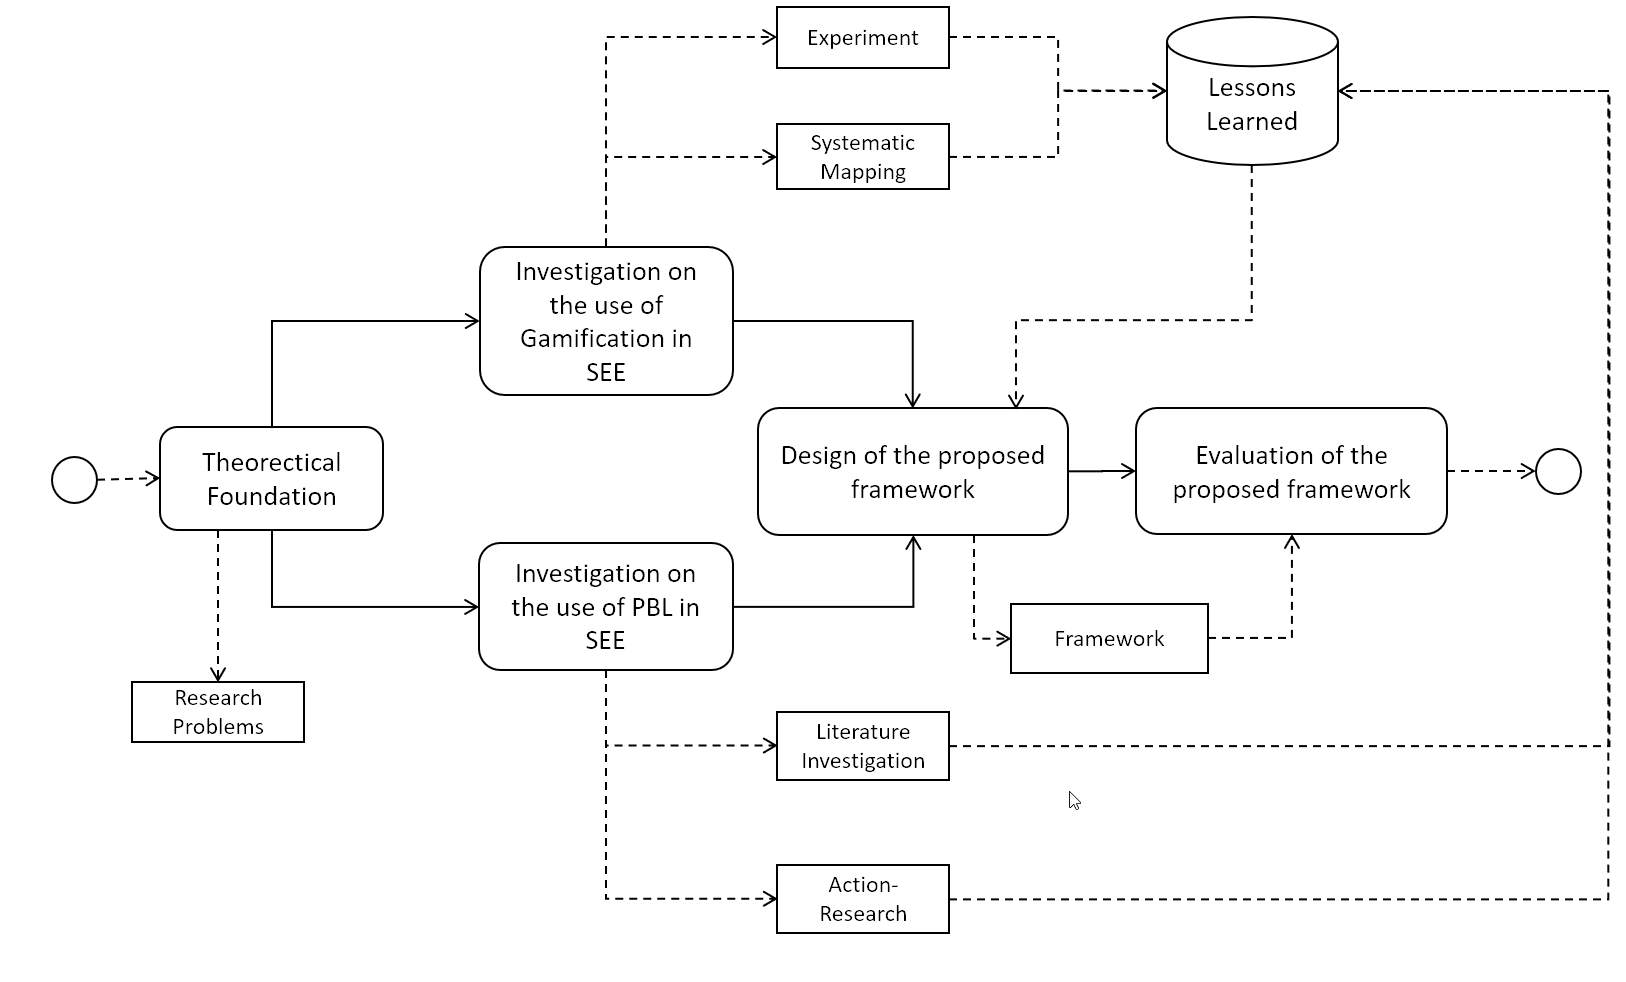
\includegraphics[width=1\textwidth]{img/method.png}
\caption{Study design}
\label{fig:method}
\end{figure} 

\section{Contribution and Relevance}
\label{sec:contribution}

The main expected contribution of this thesis is the documentation of a framework for the gamification of project-based software engineering education. This product is expected to provide educators with a reusable method and guidelines to support the introduction of educational software projects as practical assignments in SE related courses, grounded in lessons learned from theory and practice on the use of Gamification and PBL.

The relevance of this study relies on the growing demand for development of professional competences on undergraduate SE students, the recurring challenge of balancing theory and practice in SE education. As a byproduct of this thesis, this research contributes with additional options for the introduction of Gamification and PBL in SE education. Additionally, a recurrent problem stated in the literature on Gamification in SE education is the shortage of empirical evidences of the use of this technique. Therefore, the relevance and contribution of this thesis also resides in providing empirical data regarding the use of PBL and Gamification.

Until the date of production of this document, the following publications were byproducts of this thesis project:

\begin{itemize}
    \item Mauricio R. de A. Souza, Lucas Veado, Renata Teles Moreira, Eduardo Figueiredo, Heitor Costa. A Systematic Mapping Study on Game-related Methods for Software Engineering Education. Information and Software Technology (IST), ISSN 0950-5849, DOI:10.1016/j.infsof.2017.09.014. 2018.
    \item Maurício R. A. Souza, Lucas Veado, Renata Moreira, Heitor Costa, Eduardo Figueiredo. Games for Learning: Bridging Game-related Education Methods to Software Enginering Knowledge Areas. 39th International Conference on Software Engineering (ICSE), Software Engineering Education and Training (SEET) track. DOI: 10.1109/ICSE-SEET.2017.17. Buenos Aires, Argentina, 2017.
    \item Maurício R. A. Souza, Kattiana Constantino, Lucas Veado, Eduardo Figueiredo. Gamification in Software Engineering Education: An Empirical Study. 30th International Conference on Software Engineering Education and Training (CSEE\&T).  DOI: 10.1109/CSEET.2017.51. Savannah, GA, USA, 2017.
\end{itemize}

This project also resulted in the following presentation:

\begin{itemize}
    \item Maurício R A Souza, Renata Moreira, Eduardo Figueiredo. A Framework for the Gamification of Practical Assignments in SE Education (Poster). 30th International Conference on Software Engineering Education and Training (CSEE\&T). Savannah, GA, USA, 2017.
\end{itemize}

The following research papers have been submitted for conferences:

\begin{itemize}
    \item \textbf{Games and Gamification in Software Engineering Education: A Survey with Educators} - The results of survey with 83 software engineering professors from Brazilian universities regarding the adoption of game-related approaches in software engineering education.
    \item \textbf{Giving the Game Away: A Detailed Study of Game Elements} - The identification of the main game elements used to support software engineering activities (both in academia and industry), and proposal of a conceptual framework for their adoption.
    
\end{itemize}

\section{Thesis Project Outline}
\label{sec:outline}

In addition to this introductory chapter, Chapter 2 provides the essential concepts related to the research. Chapters 2, 3 and 4 presents investigations on the use of specific learning methods in software engineering education. Chapter 5 delineates the initial documentation of the framework proposed in this thesis project. The details on each chapter is presented as follows:\\

\noindent
\textbf{Chapter~\ref{ch:background}} presents background information to support the comprehension of this thesis project. It includes the main concepts related to software engineering education, learning methods adopted in SE education to support practice, and game-related methods used in SE education. This chapter also discusses related work.\\

\noindent
\textbf{Chapter~\ref{ch:sms}} presents the protocol and results of a systematic mapping study performed to identify the state-of-the-art literature on game-related educational methods to support software engineering education.\\

\noindent
\textbf{Chapter~\ref{ch:gamificationExperiment}} describes an empirical study on the adoption of Gamification in an introductory software engineering education.\\

\noindent
\textbf{Chapter~\ref{ch:actionResearch}} presents an Action-Research study describing the adoption of PBL in an introductory software engineering course and reports the lessons learned from this study.\\

\noindent
\textbf{Chapter~\ref{ch:framework}} presents the initial outline of the proposed framework to support the gamification of project-based software engineering education.\\ 

\noindent
\textbf{Chapter~\ref{ch:conclusion}} presents the conclusion of this thesis project, summarizing the status of the project, next steps, and the main lessons and issues found until the moment of conclusion of this document.
\chapter{Background and Related Work}
\label{ch:background}

\section{Software Engineering Education}

\subsection{Game-related approaches in SE Education}


\begin{table}[htb]
\caption{Knowledge Areas from \cite{Acm:2015}}
\label{table:knowledgeareas}
\centering
\scriptsize
\begin{tabularx}{\textwidth}{>{\hsize=.3\hsize}X>{\hsize=.7\hsize}X>{\hsize=2\hsize}X}
\hline
\textbf{Acronym} & \textbf{Name} & \multicolumn{1}{c}{\textbf{Description}}  \\
\hline
MAA              & Software Modeling and Analysis          & Modeling and analysis can be considered core concepts in any engineering discipline because they are essential to documenting and evaluating design decisions and alternatives.                                                           \\
REQ              & Requirements Analysis and Specification & The construction of requirements includes elicitation and analysis of stakeholders’ needs and the creation of an appropriate description of desired system behavior and qualities, along with relevant constraints and assumptions.       \\
DES              & Software Design                         & Software design is concerned with issues, techniques, strategies, representations, and patterns used to determine how to implement a component or a system.                                                                               \\
VAV              & Software Verification and Validation    & Software verification and validation uses a variety of techniques to ensure that a software component or system satisfies its requirements and meets stakeholder expectations.                                                            \\
PRO              & Software Process                        & Software process is concerned with providing appropriate and effective structures for the software engineering practices used to develop and maintain software components and systems at the individual, team, and organizational levels. \\
QUA              & Software Quality                        & Software quality is a crosscutting concern, identified as a separate entity to recognize its importance and provide a context for achieving and ensuring quality in all aspects of software engineering practice and process.             \\
PRF              & Professional Practice                   & Professional practice is concerned with the knowledge, skills, and attitudes that software engineers must possess to practice software engineering professionally, responsibly, and ethically.                                            \\
\hline
\end{tabularx}
\end{table}


\subsection{Practical approaches for SE Education}

\section{Project-based Learning - PBL}

One strategy that has been largely used to overcome these challenges is the introduction of software projects in software engineering education (eg.: capstone and project-based courses) (delgado17, marques17). In this context, project-based learning is one of the main successful student-centered pedagogies broadly used in computing science, information systems and engineering courses (marques17, macias12, Jazayeri15, Delgado17, shuto16, warin16, yamada14).

Project-based learning (PBL) is a comprehensive approach to classroom teaching and learning where students are engaged in the investigation of realistic problems, and they learn by working on an open-ended project, discovering problems and finding solutions as they go along. (Blumenfeld91, Jazayeri15). Bender (Bender12) describes PBL as an instructional model based on having students confront real-world issues and problems that they find meaningful, determine how to address them, and then act in a collaborative fashion to create problem solutions. In PBL, the instructor has a less central role, acting as a guide, and students take more responsibility for their own learning, which results in higher student involvement (Martin14, Jazayeri15).

Many software engineering courses use projects as assignments to give students a chance to experience practical problems. However, Jazayeri et al (Jazayeri15) states that this is not enough to implement a PjBL, as these projects are not typically open-ended, and students are expected to follow a very specific path to the solution. Therefore, students are not in charge of learning in these scenarios. In PjBL, projects drive the learning process, and learners should face meaningful problems, where they can investigate, apply and reflect on knowledge and skills useful to solve it. The educator moves from the role of knowledge provider, to the role of facilitator, providing meaningful feedback on students’ actions, helping students to reflect, and providing sufficient guidance for students to achieve learning outcomes.

Gary (Gary15) suggests that in PjBL, “real-worldedness” is achieved by leading students to identify key decision-making factors and draw upon prior experiences. Therefore, while traditional homework and other learning approaches have their significance, PjBL provides more durable benefits, regarding engagement, integration of methods and techniques learned in different courses, and the development of teamwork (Gary15, Warin16). Additionally, sustained interaction over time ensures that students continuously apply and evaluate these experiences (Jazayeri15).

However, there are some challenges related to the use of PBL in SE education. The following subsections address these challenges and issues.

\subsection{PjBL as an Educational Method}

Regarding the adoption of PjBL approaches in SE education, Martin et al (martin14) point issues faced by instructors and by students. Regarding the instructor role, the authors suggests that (martin14): “teachers find difficulties in designing PBL activities that fulfill the main characteristics of this methodology” [PL33], and “Other difficulties are related to the new teachers’ role, where they have to change from a knowledge transmitter to a guide or facilitator, losing control on the student work” [PL35]. Regarding the learner role, the authors points that “In some academic contexts, students are not used to dealing with this kind of problems, therefore they feel lost and end up rejecting the methodology” [PL34].

Warin et al (warin16) mention the lack of comprehensive methodologic frameworks to support educators in setting up courses using this learning method [PL17].  The authors also compare the situation of PjBL and PBL (Problem Based Learning), claiming that while they did not find articles in the literature proposing complete PjBL methods, there are well-established generic methods for PBL that are broadly applicable. Warin et al (warin16) and (macias12) also point the need of tools to support this learning method [P12].

Finally, Yamada et al (yamada14) discuss the issues related to the assessment of the educational effectiveness of this learning method [PL28]. Yamada et al (yamada14) break down this issue as four problems: Obscurity of educational effectiveness, quantitative measurement of the education process, difficulty in quantifying personal characteristics, and difficulty in determining the learning process.

\subsection{Setup of PjBL courses}

The most recurring issue found was that preparing and running PjBL course is time, resource, and effort consuming, both for educators and learners [PL04] (harms16, Hanakawa15, Nguyen13, marques18, Rupakheti17, Daun16, gary15, Mäkiö17). From the instructors perspective, PjBL requires considerable effort to supervise, guide and mentor students over a significant period of time (gary15, Daun16). There is also investment in setting up proper projects for students to tackle (Rupakheti17). For students, PjBL ensures sustained, long-term participation, what is contrary to bursty nature of students (gary15). However, they may not be able to devote the necessary time and effort because they may have other subjects to study at the university (hanakawa15).

Other problems that are directly associated to PL04 are: PjBL requires some level of preparations [PL22], as instructors are required to produce lecture material, academic examples, or project milestones (Daun16); instructors may need to specify a process that allows students to reach their learning outcomes [PL14]; some projects require setting up adequate development environments [PL02]  and physical space [PL24]; finally, some learning outcomes may require proper selection of state of art tools that student should use during the execution of their projects [PL16]. 
All those issues impact on scalability [PL03]. Scaling PBL is difficult both in terms of student head count and integration across the degree program (gary15). For instance, Harms et al (Harms16) claims that there is a limit to the number of student-led projects that an instructor can manage, and in their experience, using student-led projects with a class of more than 30 students was hard to manage.

\subsection{Selection of meaningful projects}

In PjBL, projects play a central role in the learning process. Therefore, the selection of adequate projects for students’ immersion is a crucial step in the setup of PjBL courses. The selection of projects that provide good balance in size, complexity and type of stakeholders [PL05] is a challenge that educators are exposed to. Harms et al (harms16) states that “projects need to not be too shallow and yet not be too idealistic either”.

As a consequence, there is a discussion on the use real versus realistic projects, i.e. the use of real projects from the community or industry, where real customers act as stakeholders, versus the use of projects that simulate real problems, where instructors play the role of customers or problem providers. In the former, educators must face the problems of the difficulty in establishing partnerships with the industry [PL20], as the immediate rewards and time availability for industry practitioners to collaborate in instruction are quite limited, there might be restrictions related to intellectual property, and there is no guarantee for successful outcomes for companies (daun16). Additionally, the participation of external person as real customers may be problematic [PL30], as their availability and expectations are not controlled.

In the case of educators acting as stakeholders [PL21], Daun et al (daun16) warns:
“(…) this requires a high sensitivity and  experience of the instructors regarding their ability to foresee student challenges, maintain the acted role throughout the semester, and carefully guide the knowledge discovery process in such a way that the students achieve teaching goals and perform satisfactorily. Moreover, this also requires a large amount of in-depth industry knowledge, which unless the instructor has an industry background, may not be attainable. Furthermore, the instructor will continuously have to switch between both rolls (i.e. stakeholder and teacher). Hence, there is a threat that students will take statements given by the stakeholder falsely as instruction or solution given by the teacher.” (daun16).

Nguyen et al (Nguyen13) described a problem regarding the use of real problems, where students who worked on small components of very large-scale projects in some IT companies. The authors claim these students did not have a big picture of what they were working on, and thus did not realize much benefit of their IT skills and knowledge. Therefore, the choice of projects may impact in the coverage of expected learning outcomes [PL10]. However, we believe that this problem is not specific to the context of real projects, as we discuss it further in section IV-D.

Finally, it is important that the projects are chosen considering aspects such as the relevancy of the application domain [PL15]. The choice of application domain must balance student excitement and relevancy for industry, however, this is a hard choice, as relevancy in this context may be volatile trends (delgado17). 

It is important to consider that PjBL deals with ill-structured problems as central activities [PL21], which Martin et al (martin14) consider is one of the cornerstones of PBL and one of the main sources of difficulties in using PBL. In ill-structured problems, one or more of the problem elements are unknown or not known with any degree of confidence, goals are vague or unclear, there are multiple solutions and solution paths (or even no consensual solution), they present uncertainly about which concepts, rules and principles are necessary, learners are required to express personal opinion, beliefs or judgments. This may lead back to problem PL34.

\subsection{Tracking students progress and learning outcomes}

Considering the nature of PjBL activities, there is the issue of requiring the right amount of guidance towards learning outcomes [PL25]. Considering the open-ended nature of the activities, no two projects or project teams are the same, so each student has different experience (gary15). However, the learning outcomes remains the same for everyone, and instructors have to keep close attention on keeping students on track of the learning goals. 

Considering problems PL15 and PL25, instructors are required to spend considerable effort in tracking students progress and providing meaningful feedback for students to ensure learning [PL01]. Tracking the progress of students projects is not easy, as instructors are required to scrutinize the report by students or participate in projects in order to understand progress of the projects, what forces educators to bear the burden (Fukuyasu13). Instructors also have to be aware of the risk of students unethically using source code of others and claiming its their own work [PL06]. 

Consequently, the definition of a strategy to evaluate students is also difficult [PL18], as it may require considering qualitative and quantitative data on their performance. If not clearly defined, students may become confused and concerned regarding their assessment [PL23]. As students direct their activities based on the given assessment criteria [11], the assessment design plays a key role in what students will focus on [Fagerholm13]. 

Educators must consider that the projects should be aligned with expected learning outcomes (as discussed on in PL10 in previous section). In technical domains, such as mathematics or computer science, it may be difficult to instruct a variety of largely independent but closely related concepts and topics (daun16). Therefore, a challenge arises when dealing with instructing instruct complex theoretical relationships in a sound fashion [PL19]. In software engineering, for instance, software process is a transversal knowledge, and each of the phases of software development life cycle, is closely related to the other, however each one has a multitude of learning topics. It is difficult to impart the importance of each topic and the impact they have on each other.

Additionally, students may become absorbed by a single facet of the project, such as programming [PL08]. Hanakawa et al (hanakawa15) illustrate this matter in their first attempts to introduce contest-based learning, where the students became absorbed in programming rather than design and analysis activities. Similarly, Winterfeldt14 describe their experiences using a project-based approach of teaching application design. However, they recognized as a general challenge that students focus on details of an implementation (technology and coding) rather than on the application structure (Architecture and design).

Finally, when students have to interact with new technologies, they may get overwhelmed when searching for relevant instructional materials [PL13], 


\subsection{Teamwork and different types of learning}

Although PjBL does not necessarily involves team activities, it has been largely used in software engineering education to support practicing soft skills such as teamwork, communication, leadership, and collaboration. Specific topics related to software process or software project management also benefit from projects executed in teams. Therefore, some authors suggest that instructors should plan carefully about team composition [PL26], as teams composed by members with the right complementary skills may improve the learning experience, while others compositions may compromise it (sunaga16, sunaga17, yamada14).

Besides that, students working in teams may be affected by their lack of teamwork experience [PL11]. Chen14 state that “if not equipped with the necessary teamwork skills, these students are like blind explorers trying to find the proper direction in which to take their project”. The authors support that the lack of team experience impedes learning and makes it difficult to obtain quality results. 
Kizaki14 mentions other problems related to teamwork: shortage of communication between members [PL29] and difference of a member's technical capabilities [PL31]. The later, may also impact in the problem of a heterogeneous effort distribution among team members [PL32], what may lead to knowledge not being equally distributed [PL09]. As a consequence, it becomes even harder to individually assess students progression toward learning outcomes, due “to the ingenuity some students show in hiding behind others’ work” (gary15).

Finally, students are impacted differently by the teaching approach, as they may have different learning styles (zhi16). Therefore, a challenge using PjBL is to address different learning styles of students [PL07], which may require mixing different learning environments, resources, modes and/or contents.



\section{Gamification}

\section{Related Work}

\section{Final Remarks}
\chapter{A Systematic Mapping Study on Game-related Methods for Software Engineering Education}
\label{ch:sms}

The goal of this chapter is to identify and discuss game-related methods in the context of software engineering education. We call game-related methods for software engineering education, any approach where games are used to support the process of teaching or learning software engineering. Therefore, we conducted a systematic mapping study to survey the software engineering education literature in order to: (i) identify game-related methods for software engineering education; (ii) understand how these game-related methods support the software engineering knowledge areas from SE 2014; and (iii) understand specific characteristics of each game-related method. 

Previous studies \citep{Marques:2014, Malik:2012, Caulfield:2011, Kosa:2016} investigated and mapped educational methods in the software engineering education context. This study complements previous ones by providing the following novel contributions to the community. First, we propose a classification scheme for game-related educational methods used in software engineering education. Second, we analyze the difference in the proposal and application of methods found in the literature. Third, we also discuss how these educational methods support specific software engineering education knowledge areas.

From the 156 primary studies analyzed, we identified three game-related methods used in software engineering education: “Game-based Learning”, “Game Development Based Learning”, and “Gamification”. We mapped their learning goals and identified that these educational methods are mostly used to support the knowledge areas of “Software Process”, “Software Design” and “Professional Practice” (as described in \cite{Acm:2015}). However, each educational method has different purposes and rationales to support these knowledge areas, thus serious games are more used in the context of “Software Process” education, while “Game Development Based Learning” is more used in “Software Design” education. Gamification in software engineering education is new, and initial results are promising, however, further investigation and additional empirical evidences are still needed for the discussion of its effectiveness in this context.

The remainder of this chapter is organized as follows. Section 2 provides the necessary theoretical foundation for the study. In Section \ref{sec:smsstudySettings}, we describe the design of this systematic mapping study. Section \ref{sec:smsresults} presents the results of the study and Section \ref{sec:smsdiscussion} discusses the results and provides insights about the role of each game related method in software engineering education. In Section \ref{sec:smsthreats}, we discuss the threats to the validity of the study. Section \ref{sec:final} concludes this research paper.

\section{Study Settings}
\label{sec:smsstudySettings}

This section presents the goals of this study and the methodology adopted. Section \ref{sec:smsgoals} presents the study goal and research questions. Section \ref{sec:smsmethod} explains the research method and the process executed. Section \ref{sec:smssearch} discusses the search strategy applied to mine relevant scientific databases. Section \ref{sec:smsselection} shows the selection process filtering only relevant papers for this study. Section \ref{sec:smsdataextraction} presents the classification scheme and mapping strategy used to present the study results.

\subsection{Goal and research questions}
\label{sec:smsgoals}

The goal of this study is to identify and analyze game-related methods from the purpose of understanding their application and learning objectives in the context of software engineering education. To achieve this goal, we established five research questions:

\textbf{RQ1.} What game related methods have been proposed for supporting software engineering education?

\textbf{RQ2.} What software engineering education knowledge areas are supported by the existing game-related methods?

\textbf{RQ3.} What game elements have been used for the Gamification of software engineering education? 

Based on the classification scheme for game-related methods for software engineering education [5], the expected outcome of RQ1 is a list of primary studies categorized by approach type. The expected outcome of RQ2 is a mapping between learning objectives from the approaches identified in RQ1 and the software engineering knowledge areas from SE 2014. Finally, the expected outcome of RQ5 is a summary of game elements, mechanics, and dynamics extracted from the list of Gamification approaches identified in RQ1.

\subsection{Method}
\label{sec:smsmethod}

To achieve the study goal, we have conducted a Systematic Mapping Study (SMS). SMS is a secondary study method that systematically (i.e., based on a structured and repeatable process or protocol) explores and categorizes studies in a given research field, and provides a structure of the type of research reports and results that have been published \citep{Petersen:2007}[20]. SMS results are often organized as visual summaries (maps). The expected contribution is to provide researchers and educators with an overview of the state-of-the-art on the use of games and game elements for supporting software engineering knowledge areas from the educational perspective. Additionally, we expect to identify possible research gaps and trends.

We have conducted the SMS in the period of June/2016 to December/2016, following four process steps adapted from Petersen et al. \citep{Petersen:2007} (Figure \ref{fig:smsprocess}).

\begin{figure}[!h]%th
\centering
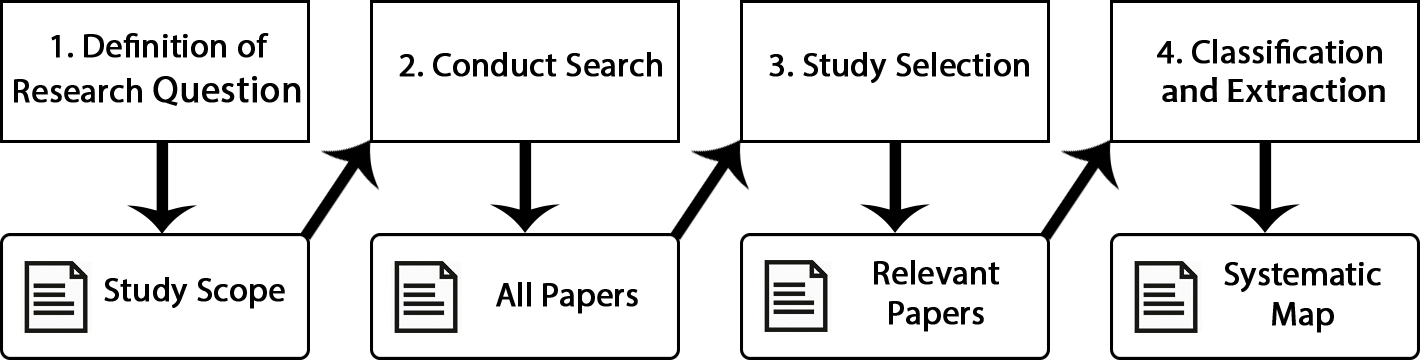
\includegraphics[width=0.8\textwidth]{img/smsprocess.png}
\caption{Systematic mapping process, adapted from \cite{Petersen:2007}}
\label{fig:smsprocess}
\end{figure} 

\textbf{Step 1} – Definition of research questions: We have defined five research questions based on the study goal, to establish the desired scope of the systematic study (Section \ref{sec:smsgoals});

\textbf{Step 2} – Conduct search: based on the research questions, we defined and performed a replicable process for searching for retrieving papers in selected scientific databases (Section \ref{sec:smssearch});

\textbf{Step 3} – Study Selection: We have defined and applied a replicable process for selecting only the relevant papers for this study (Section \ref{sec:smsselection});

\textbf{Step 4} – Study Classification and Data Extraction: Based on the research questions, we have defined a strategy for mapping the relevant data from the primary studies (Section \ref{sec:smsdataextraction}) and for presenting the study results (Section \ref{sec:smsresults}). 

Five researchers participated in the planning and execution of the study: an undergraduate student in CS, a PhD student in CS, and three PhD associate professors teaching software engineering courses in two different institutions.

\subsection{Search strategy}
\label{sec:smssearch}

The search strategy enables the inclusion of relevant studies in the search results. To identify possible primary studies for data extraction, the search was based on (i) trial searches using combinations of keywords derived from the study goal for the definition of valid search strings and (ii) the execution of automatic searches in the scientific databases using the search strings. 	Initially, we selected relevant keywords related to the three domains under analysis: (a) education; (b) software engineering; and (c) game-related approaches. In order to identify these relevant keywords, we considered search strings used in related systematic studies, bodies of knowledge and curricula guidelines for software engineering, and experts (software engineering educators). The resulting keywords per domain were:

\textbf{Education:} teach, learn, education, train;

\textbf{Software engineering:} software engineering, software process, software requirements, requirements engineering, software verification, software validation, software design, software architecture, software test, software quality, software project management;

\textbf{Game-related approaches:} game, serious games, edutainment, gamification, game based learning, gbl.

Search strings were defined by grouping keywords in the same domain with the logic operator “OR” and grouping the three domains with the logic operator “AND”. We then executed automatic searches in four selected scientific databases, using and adapting (when necessary) the search string. The databases used were ACM Digital Library , IEEE Xplore , EI Compendex , and Scopus , since they have a large amount of relevant conferences and journals indexed. We limited the results of automatic searches to return only papers written in English, and we did not apply any time limitation.

\subsection{Study selection}
\label{sec:smsselection}

In this step, we filtered the studies retrieved from the automatic searches by some steps to exclude papers not aligned with the study goals. First, the five researchers defined the following inclusion and exclusion criteria:

•	Inclusion Criteria: Studies whose main focus was on proposal, usage, discussion or evaluation of game-related methods in the context of software engineering education;

•	Exclusion Criteria: Papers not written in English; Papers not fully available to download; Studies formatted as short papers (2 or less pages), tutorials, demos, books, book chapters, and similar; secondary studies; and duplicated studies.

The study selection process was executed in two phases: (i) in the first selection phase, two researchers individually read all titles and abstracts and removed studies that did not comply with inclusion criteria; (ii) in the second selection phase, they have downloaded all remaining papers and each researcher examined all papers’ introduction and conclusion to remove studies that matched the exclusion criteria. During these steps, any conflict was solved with a third researcher. For any persisting problem, the two remaining researchers were consulted for a final decision regarding the inclusion or exclusion of a primary study. However, only a few conflicts emerged in the first selection phase (less than 7\% of the selected studies), and most cases because the learning topic was not clearly related to software engineering. In the second selection phase, those conflicted studies were carefully read and the third researcher helped in the decision of inclusion or exclusion. Therefore, we believe the selection process is clear and precise enough for replication.

Table \ref{table:studyseleciton} summarizes the result of the selection process. The first column (Source) presents the scientific databases mined and the second one (\# Papers) describes the number of papers retrieved from the use of the search strings. The third (1st Selection) and fourth (2nd Selection) columns shows the number of remaining papers after the execution of the first and second selection phases, respectively. The fifth column (\% Included) describes the ratio between the remaining papers after the selection process (2nd Selection) and the total number of papers retrieved from each database (\# Papers). Finally, the last column (Interval) presents the time range of the resulting primary studies.


\begin{table}[htb]
\caption{Results of the study selection process}
\label{table:studyseleciton}
\centering
\newcolumntype{Y}{>{\centering\arraybackslash}X}
\scriptsize
\begin{tabularx}{\textwidth}{>{\hsize=.35\hsize}X>{\hsize=.3\hsize}Y>{\hsize=.35\hsize}Y>{\hsize=.35\hsize}Y>{\hsize=.3\hsize}Y>{\hsize=.3\hsize}Y}
\hline
\textbf{Source} & \textbf{\# Papers} & \textbf{1st Selection} & \textbf{2nd Selection} & \textbf{\% Included} & \textbf{Interval}  \\ \hline
ACM DL       & 1204      & 248           & 42            & 3,49\%      & 1974-2016 \\
IEEE Xplore  & 558       & 155           & 69            & 12,37\%     & 1977-2015 \\
EI Compendex & 1133      & 313           & 120           & 10,68\%     & 1982-2016 \\
Scopus       & 1270      & 336           & 132           & 10,47\%     & 1974-2016 \\
Total        & 4165      & 1052          & 363           & 8,72\%      & 1974-2016 \\
Total*       & 2675      & 568           & 156           & 5,83\%      & 1974-2016 \\
\hline
\end{tabularx}
\end{table}

The study selection process resulted in 156 unique primary studies. However, we found a high number of duplicates among different scientific databases. Figure \ref{fig:smsdistribution} illustrates the overlapping results between databases. We removed the duplicated papers from the results of the automatic search (\# Papers). However, for the purpose of documentation and analysis, we kept track of the database from where each paper was found. 

\begin{figure}[!h]%th
\centering
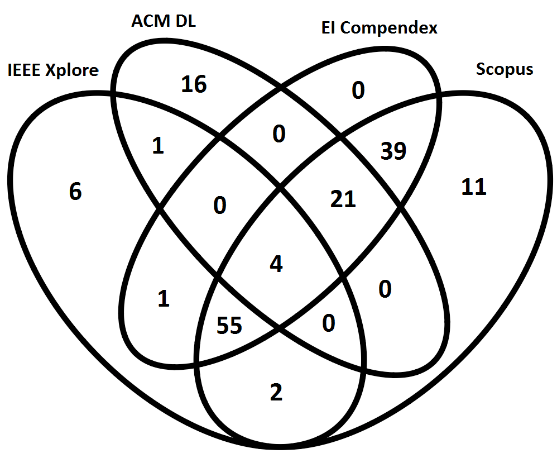
\includegraphics{img/smsDistribution.png}
\caption{Distribution of Primary Studies per Database.}
\label{fig:smsdistribution}
\end{figure} 

\subsection{Study classification and data extraction}
\label{sec:smsdataextraction}

We analyzed the resulting list of primary studies for extracting information by identifying: (i) the presented approach; (ii) the game-related method used; and (iii) learning objectives or expected developed skills. We classified each approach using game-related methods (RQ1) in the following categories [5]: Gamification, GBL, and GDBL (as described in Section 2.2). 	We then identified the expected learning outcomes and mapped them to the purpose and related topics of the knowledge areas from SE 2014. 

\section{Results}
\label{sec:smsresults}

In this section, we presented the results of the systematic mapping study. Section \ref{sec:smsresultoverview} provides an overview of the primary studies selected for this study. Sections \ref{sec:smsrq1} to \ref{sec:smsrq3} describes the results for the research questions RQ1 to RQ3, respectively.

\subsection{Overview}
\label{sec:smsresultoverview}

The study selection resulted in 156 primary studies, published between 1974 to June 2016. Figure \ref{fig:smstimeline} presents a histogram with the frequency of primary studies per year, with different colors representing the types of approaches found (discussed in details in Subsection \ref{sec:smsrq1}). This result suggests that software engineering education has been a challenge since the early years of software engineering in the 1970’s, and that the use of game-related educational methods is not a novelty. Nonetheless, since 2002 there has been a constant and growing presence of studies about the use of game-related methods for software engineering education.

\begin{figure}[!h]%th
\centering
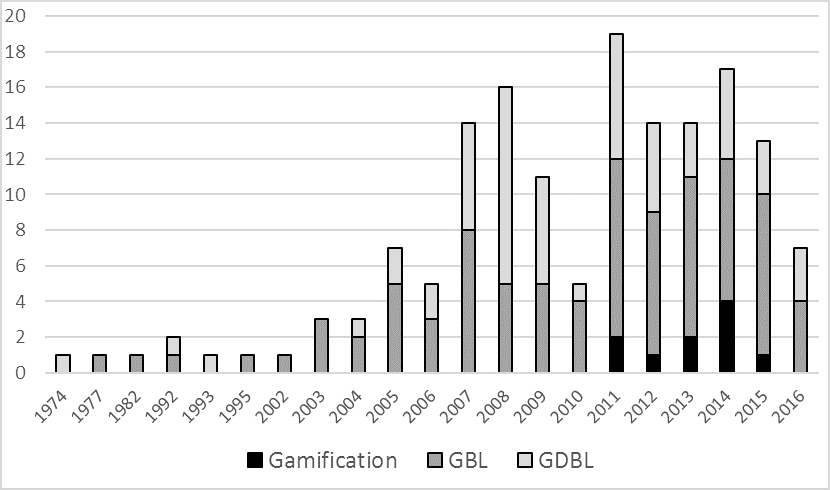
\includegraphics{img/smsTimeline.png}
\caption{Timeline of primary studies.}
\label{fig:smstimeline}
\end{figure} 

Figure \ref{fig:smsforum} shows the distribution of studies per type of forum. The majority of the primary studies was published in conferences (69\%), but we also retrieved studies from journals (24\%) and workshops (7\%). The conferences with greater occurrences of primary studies were CSEE&T, FIE, SIGCSE, and ICSE. Table \ref{table:publicationvenues} summarizes the most recurring publication venues in our study and their respective counting of selected primary studies. We list the publication venues that have three or more primary studies selected in this study. Appendix A provides the complete list of primary studies. In the remainder of this paper, we used unique identifications (PS<number>) when referring to primary studies.

\begin{figure}[!h]%th
\centering
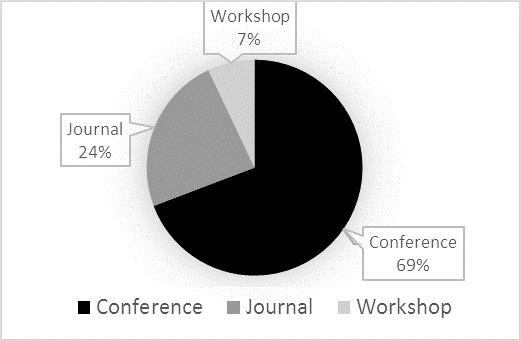
\includegraphics{img/smsForum.png}
\caption{Distribution of primary studies per type of forum.}
\label{fig:smsforum}
\end{figure} 

\begin{table}[htb]
\caption{Relevant publication venues for game related approaches in software engineering education}
\label{table:publicationvenues}
\centering
\newcolumntype{Y}{>{\centering\arraybackslash}X}
\scriptsize
\begin{tabularx}{\textwidth}{>{\hsize=.15\hsize}Y>{\hsize=.8\hsize}X}
\hline

\textbf{\# Studies} & \textbf{Publication Venues}                                                       \\
15         & IEEE Conference on Software Engineering Education and Training (CSEE\&T) \\
13         & Frontiers In Education Conference (FIE)                                  \\
11         & ACM Technical Symposium on Computer Science Education (SIGCSE)           \\
10         & International Conference on Software Engineering (ICSE)                  \\
5          & Journal of Computing Sciences in Colleges                                \\
4          & IEEE Transactions on Education                                           \\
4          & IEEE Global Engineering Education Conference (EDUCON)                    \\
3          & International Conference on Computer Games (CGAMES)                      \\
3          & International Workshop on Games and Software Engineering (GAS)           \\
3          & International Journal of Computer Games Technology                       \\
3          & ASEE Annual Conference and Exposition         \\            

\hline
\end{tabularx}
\end{table}

\subsection{RQ1 – Game-related methods for software engineering education}
\label{sec:smsrq1}

This section discusses the results for the first research question  \textit{RQ1. "What game-related methods have been proposed to support software engineering education?"}.

In accordance to the classification described in Section 3.5, 88 primary studies presented the use of GBL method, 60 presented the use of GDBL method, and 11 presented Gamification approaches. Three primary studies presented hybrid approaches, i.e., the combination of two distinct methods: (i) one used Gamification and GDBL; and (ii) two used GDBL and GBL. Table \ref{table:smscategories} presents the mapping of game-related methods found (Method), the primary studies that use each method (Primary Studies) and their quantity, and the number of studies that have some sorts of evaluation in the classroom.
 
\begin{table}[htb]
\caption{Mapping of categories of game-related methods and primary studies}
\label{table:smscategories}
\centering
\newcolumntype{Y}{>{\centering\arraybackslash}X}
\scriptsize
\begin{tabularx}{\textwidth}{>{\hsize=.3\hsize}X>{\hsize=.25\hsize}Y>{\hsize=.25\hsize}Y>{\hsize=.25\hsize}Y}
\hline
\textbf{Method}       & \textbf{Primary Studies} & \textbf{\# Primary Studies} & \textbf{Evaluation} \\ \hline
Gamification          & PS001 - PS010            & 10 (6.4\%)  & 6 (60\%)            \\
GBL                   & PS011 - PS096            & 86 (55.1\%) & 45 (52,3\%)         \\
GDBL                  & PS097 - PS153            & 57 (36.5\%) & 18 (31,6\%)         \\
Gamification and GDBL & PS154                    & 1 (0.6\%)     & 0                   \\
GBL and GDBL          & PS155 - PS156            & 2 (1.2\%)   & 1 (50\%)       \\    
\hline
\end{tabularx}
\end{table}

GBL and GDBL are the most prevalent methods found in this study. Both methods are used to support software engineering education since the decade of 1970’s (PS082, PS143). GBL approaches include serious games and non-serious games in digital or non-digital formats. Some examples of serious games include GetKanban (PS087), PMG-2D (PS071), and InspectorX (PS055), designed to support the learning of Kanban, project management and software inspection, respectively. The use of games as learning tools (GBL approaches) is usually motivated by the opportunity of teaching learning topics difficult to explore in traditional lectures. This difficulty is often caused by limitations imposed by the nature of the topic, by time restrictions of traditional lectures or by practical problems related to real life experiences hard to translate to examples in the classroom. For instance, Smart Decisions (PS080) is a game developed to aid in teaching architecture design. \cite{Cervantes:2016} suggest “software architecture courses frequently rely on relatively simple examples (…) Such examples may present the essential concepts of design, but they are also distant from real life system design experiences”. The authors also suggest that the timeframe is too short to observe consequences of the decisions that are made as part of the design process \citep{Cervantes:2016}. Therefore, games are useful to support the setup of a controlled environment that can simulate real life experiences. 

Primary studies proposing the use of GDBL method are divided in two types: (i) assignments on developing game products; and (ii) adoption of game development frameworks. The former studies describe experiences of students’ assignment with hands-on experience in the domain of game development to introduce the challenges of software engineering. For instance, PS111 describes and evaluates a block course in which students with almost no mobile application development experience create games in just two weeks. These students learn modeling, design patterns, software configuration management, and game development. PS123 employs game “play testing” for learning about issues and challenges of modern software engineering projects and practices. The later studies advocate the use of game development frameworks as learning instruments to simplify certain aspects of development (e.g., technicalities of learning a new language) and allowing students to concentrate efforts on specific learning goals (e.g. software design). For instance, PS150 describes a case study of how a game project using the XNA Game Studio from Microsoft was implemented in a software architecture course.

Concerning Gamification, although the term is recent in literature \citep{Deterding:2011}, it was rapidly incorporated in software engineering education since 2011 (PS007, PS010). Gamification approaches found are usually applied as an innovative learning context more focused in engaging and motivating learners to perform desired behaviors. However, we observed two different strategies for the use of Gamification in software engineering education: (i) Gamification of the classroom experience and (ii) Gamification of specific software engineering activities. Gamification of the classroom experience refers to the use of game elements to engage and motivate students in performing learning activities (PS003, PS004, PS005, PS008). For instance, PS005 describes the experiment of implementing Gamification techniques into software engineering and service-oriented architecture courses using Points, Leaderboards and Badges to promote competition and, consequently, to motivate students in the class activities. The strategy is focused in the Gamification of the classroom activities, and not specific software engineering related activities. 

Gamification of specific software engineering activities, on the other hand, applies game elements to motivate learners in practicing specific skills or performing specific practices (PS001, PS002, PS006, PS007, PS010). PS006 describes an experiment in which students are encouraged to make more frequent commits to version control system, in a software project course. The authors proposed a leaderboard based on the number of commits from each student, and established milestones/thresholds that would trigger messages congratulating students and teams that reached the specified number of commits. PS01 uses weekly challenges to motivate students on applying eXtreme Programming practices to their project. In this scenario, students compete for a “challenge cup” award.

Some studies (PS154, PS155, and PS156) mix the previous approaches in order to achieve better learning results (hybrid approaches). Two studies (PS155 and PS156) discuss the advantages of learning cycles where students play and develop serious games. One study (PS154) proposes a hybrid approach consisting of developing games focusing on good design, and applying a gamified strategy for testing it.

Regarding the evaluation of those studies, most of them adopt case studies or pilot studies in classroom. However, only 70 primary studies formally describe proper evaluation methods and results, regarding effectiveness in learning or perception of users: 45 (out of 86 – 52,3\%) studies on GBL method; 18 (out of 57 – 31,6\%) studies on GDBL method; 6 (out of 10 – 60\%) on Gamification; and 1 (out of 3 – 33,3\%) on hybrid approaches. The most recurring evaluation strategies rely on pre-test and post-test, and on questionnaires. The higher number of GBL studies with proper evaluation, in comparison to GDBL, may relate to the nature of GBL approaches: The evaluation of serious games can be performed in shorter periods, while the evaluation of development project requires longer periods. Consequently, this factor may impact on availability of participants and in the effort to perform comparative studies with control groups. In the case of Gamification, the total number of primary studies is low, therefore further investigation and additional empirical evidences are still needed for the discussion of its effectiveness in software engineering education.

\subsection{RQ2 - Mapping learning goals to SE 2014 Knowledge Areas}
\label{sec:smsrq2}

This section discusses the results for the following research question.

\textit{RQ2. What software engineering education knowledge areas are supported by the existing game-related approaches?}

We identified the learning goals of each primary study and mapped them to the SE 2014 knowledge areas (KA) described in Section 2.1 (Table \ref{table:kamap}). The results show that “Software Process” is the KA with the greater number of primary studies with game related approaches supporting it (92 - 59\%), followed by “Software Design” (60 – 38.5\%), “Professional Practice” (48 – 30.8\%), “Requirement Analysis and Specification” (39 – 24.3\%), and “Software Verification and Validation” (30 – 19.2\%). The least supported KA are “Software Quality” (10 – 6.4\%) and “Software Modelling and Analysis” (10 – 6.4\%).

\begin{table}[htb]
\caption{Mapping of knowledge areas (KA) from SE 2014 and Primary Studies}
\label{table:kamap}
\centering
\newcolumntype{Y}{>{\centering\arraybackslash}X}
\scriptsize
\begin{tabularx}{\textwidth}{>{\hsize=.1\hsize}Y>{\hsize=.75\hsize}X>{\hsize=.15\hsize}Y}
\hline
\multicolumn{1}{c}{\textbf{K.A.}} & \multicolumn{1}{c}{\textbf{Primary Studies}} & \multicolumn{1}{c}{\textbf{\#}} \\ \hline
PRO & PS001; PS002; PS006; PS007; PS011; PS012; PS014; PS015; PS016; PS017; PS019; PS020; PS021; PS022; PS023; PS025; PS026; PS027; PS028; PS029; PS030; PS034; PS035; PS036; PS037; PS039; PS040; PS042; PS043; PS044; PS045; PS046; PS049; PS050; PS052; PS054; PS057; PS058; PS059; PS060; PS061; PS062; PS063; PS064; PS068; PS069; PS070; PS071; PS074; PS075; PS076; PS077; PS079; PS081; PS084; PS086; PS087; PS088; PS089; PS091; PS092; PS094; PS096; PS097; PS102; PS107; PS110; PS111; PS115; PS116; PS118; PS119; PS120; PS121; PS122; PS124; PS128; PS129; PS130; PS131; PS134; PS135; PS140; PS141; PS142; PS144; PS145; PS146; PS148; PS151; PS155; PS156; & 92 (59\%)                       \\
DES & PS007; PS015; PS020; PS026; PS048; PS056; PS065; PS073; PS080; PS081; PS089; PS095; PS097; PS098; PS099; PS100; PS101; PS103; PS105; PS107; PS108; PS110; PS111; PS112; PS113; PS114; PS116; PS117; PS119; PS120; PS121; PS122; PS123; PS124; PS125; PS126; PS127; PS129; PS130; PS132; PS133; PS134; PS135; PS136; PS137; PS138; PS139; PS140; PS142; PS143; PS144; PS145; PS146; PS148; PS149; PS150; PS152; PS153; PS154; PS155;  & 60 (38.5\%)                     \\
PRF & PS007; PS012; PS013; PS014; PS015; PS017; PS018; PS020; PS025; PS026; PS030; PS031; PS043; PS061; PS064; PS072; PS081; PS085; PS086; PS090; PS091; PS097; PS099; PS102; PS106; PS107; PS110; PS111; PS119; PS121; PS124; PS128; PS129; PS130; PS134; PS135; PS139; PS141; PS143; PS144; PS145; PS146; PS147; PS148; PS151; PS152; PS155; PS156; & 48 (30.8\%)                     \\
REQ & PS007; PS013; PS014; PS015; PS017; PS020; PS026; PS032; PS043; PS047; PS048; PS051; PS053; PS078; PS090; PS093; PS097; PS101; PS107; PS110; PS114; PS116; PS117; PS119; PS120; PS121; PS122; PS123; PS124; PS128; PS129; PS130; PS134; PS140; PS142; PS145; PS146; PS148; PS155; & 39 (24.3\%)                     \\
VAV & PS007; PS010; PS015; PS024; PS033; PS038; PS048; PS055; PS066; PS067; PS083; PS107; PS109; PS114; PS116; PS119; PS120; PS121; PS122; PS123; PS129; PS134; PS142; PS144; PS145; PS146; PS148; PS152; PS154; PS155;  & 30 (19.2\%)                     \\
MAA & PS007; PS116; PS120; PS131; PS134; PS138; PS140; PS142; PS148; PS152; & 10 (6.4\%) \\
QUA & PS007; PS014; PS058; PS097; PS110; PS116; PS129; PS140; PS142; PS148; & 10 (6.4\%)                   \\
\hline
\end{tabularx}
\end{table}

The KA “Software Design” (DES), “Requirement Analysis and Specification” (REQ) and “Software Verification and Validation” (VAV) are directly linked to recurrent phases in software development lifecycle models (e.g., the phases of “Requirements”, “Design” and “Verification” in representations of the waterfall model). Consequently, the primary studies proposed learning experiences that address each of these KA specifically or setups where students experience topics related to these KA in the context of a software development process. 	Most of the primary studies mapped to the KA “Professional Practice” proposes game related approaches that directly support other KA and, as secondary goal, they encourage the development of professional or “soft” skills. These skills are usually related to dynamics of working in teams or groups, interacting with stakeholders, communication, and leadership.

We found few primary studies indicating the support for KA “Software Quality” (QUA) and “Software Modeling and Analysis” (MAA). Usually, the supporting for MAA was related to applying UML (Unified Modeling Language) in software design for documentation and analysis purposes. The supporting for QUA was related to definition and appliance of quality assurance procedures in the contexts of software process and software verification. The description of these knowledge areas \citep{Acm:2015} reflects their “supportive” nature: (i) MAA is described as “essential to documenting and evaluating design decisions and alternatives”; and (ii) QUA is described as a “crosscutting concern” and is suggested that “software quality topics must be integrated into the presentation and application of material associated with other KA”. 

Regarding the support of Knowledge Areas by each game-related method, Figure \ref{fig:smsbubble} describes a quantitative relationship between game-related methods and the coverage of each SE 2014 knowledge area. The different nature of each game-related method results in different strategies to support learning goals. The GBL approaches usually focus on few learning topics: 65 out of 88 (73.9 \%) primary studies describing GBL approaches support only one knowledge area. In contrast, 23 out of 60 (38.3 \%) primary studies describing GDBL approaches support a single knowledge area. This analysis shows that GBL approaches are, usually more specific in terms of learning goals, while the practical nature of GDBL approaches are broader.

\begin{figure}[!h]%th
\centering
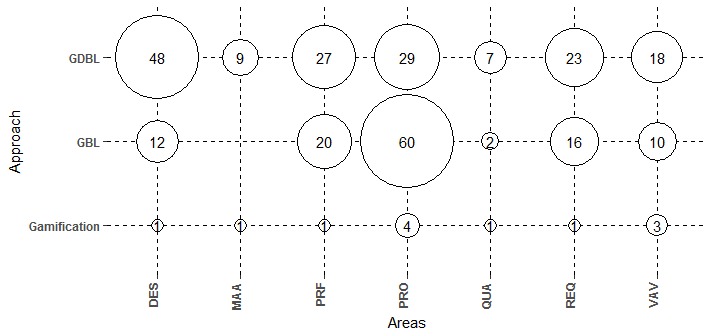
\includegraphics[width = 1\textwidth]{img/smsBubble.png}
\caption{Distribution of primary studies per type of forum.}
\label{fig:smsbubble}
\end{figure}

The mapping of Figure \ref{fig:smsbubble} also shows that “Software Design” (DES) is predominant in GDBL approaches, while “Software Process” (PRO) is predominant in GBL approaches. We observed that GDBL method favors hands-on experience on software design in a domain of systems familiar to students. The use of game development frameworks helps overcoming technology barriers (e.g. complexity of learning new programming languages) in software development, allowing students to focus on learning good design. This practical nature of GDBL approaches also reflects the higher number of primary studies supporting “Software Quality” (QUA) and “Software Modeling and Analysis” (MAA), providing learners with the experience of learning by doing.

The challenges and nuances of software process are difficult to simulate in student projects because of diverse factors (e.g., limitation of time, limitation of students’ availability). Therefore, games and simulations play a great role in creating abstractions and simplifications of real life software development.

\subsection{RQ3 - Gamification elements used in software engineering education}
\label{sec:smsrq3}

This section discusses the results for the last research question.

\textit{RQ3. What game elements have been used for the Gamification of software engineering education?}

In order to understand how Gamification is being used in the context of software engineering education, we analyzed which game elements are used in each primary study (Table \ref{table:smsgamification}). Leaderboards, Points, and Levels are the recurrent game mechanics found (5, 4, and 4 primary studies, respectively). Competition is the most recurring game design principle identified (4 primary studies).

\begin{table}[htb]
\caption{Game elements identified in primary studies}
\label{table:smsgamification}
\centering
\newcolumntype{Y}{>{\centering\arraybackslash}X}
\scriptsize
\begin{tabularx}{.8\textwidth}{>{\hsize=.5\hsize}X>{\hsize=.5\hsize}X}
\hline
\multicolumn{1}{c}{\textbf{Game Element}} & \multicolumn{1}{c}{\textbf{Primary Studies}} \\ \hline
Leaderboards                              & PS003, PS002, PS005, PS007, PS006            \\
Points                                    & PS010, PS003, PS002, PS005, PS154            \\
Milestones, Levels, Paths and Progress    & PS010, PS003, PS007, PS006, PS154            \\
Competition                               & PS001, PS003, PS005, PS007                   \\
Collaboration, Altruism, Teams            & PS010, PS003, PS007, PS154                   \\
Rewards                                   & PS010, PS003, PS154                          \\
Challenges                                & PS001, PS03                                  \\
Quests                                    & PS010, PS154                                 \\
Awards                                    & PS001                                        \\
Time Pressure                             & PS007                                        \\
Gifts \& Sharing                          & PS003                                        \\
Status                                    & PS003                                        \\
Badges                                    & PS005                                        \\
Feedback                                  & PS007                                        \\
\hline
\end{tabularx}
\end{table}


\cite{Dicheva:2015} stated that there is not a commonly agreed classification of game design elements. The analysis of the primary studies supported this claim, as we observed a lack of standard definitions of game elements. \cite{Deterding:2011} identified game elements in varying levels of abstraction and proposed a classification scheme based on 5 levels (from concrete to abstract): (i) “Game interface design patterns”; (ii) “Game design patterns and mechanics”; (iii) “Game design principles and heuristics”; (iv) “Game models”; and (v) “Game design methods”.  \cite{Zichermann:2011} categorized game elements into mechanics, dynamics, and aesthetics. \cite{Dicheva:2015} proposed a classification of game elements in gamified educational contexts organized in two levels: (i) “Game Mechanics” and (ii) “Design Principles”. The former is a combination of the first two levels of Deterding’s classification and refers to the more concrete representation of game elements, such as leaderboards, badges, point, and levels. The latter is a combination of the third and fourth level of Deterding’s classification and it is concerned with abstract elements used in games, such as Competition and Status. Therefore, given this lack of standardization in the primary studies, we did not use any of the aforementioned classification schemes. In Table 10, we mapped only the game elements as they were mentioned in the primary studies.

PS01 uses weekly challenges to motivate students on applying eXtreme Programming practices to their project. The students had to compete for a “challenge cup” award. PS010 exposes students to software testing using a game-like environment, HALO (Highly Addictive, sociaLly Optimized) Software Engineering. HALO uses MMORPG (Massively Multiplayer Online Role-Playing Game) motifs to create an engaging and collaborative development environment. Students performed software testing tasks as “quests” contextualized in a fictional storyline. When students complete “quests”, they gain “experience points” and they “level up”. Players gain Social rewards (titles and levels) when they complete achievements (such as successfully closing over 500 bugs). Students can track their progress and choose the quests they want to perform in any order. Quests can be individual or requiring a developer to form a team and work collaboratively towards their objective. HALO is also used in the hybrid approach described in PS154.

PS007 describes eight MMORPG elements incorporated in a project based software engineering capstone course: (i) Narrative Context (Epic Story); (ii) Feedback; (iii) Reputations; (iv) Rank, and Levels; (v) Marketplaces and Economies; (vi) Competition under explicit and enforced rules; (vii) Teams; and (viii) Time Pressure. In PS03, the authors provided in depth details of the setup for a gamified classroom for the subject of software engineering. The authors developed a software platform to support game elements in the classroom, such as, Paths, Purpose, Autonomy, Levels, Progress Bar, Points, Heroes, Peers, Interaction, Collaboration, and Personas. The authors did not introduce Gamification to the software engineering topics being taught, but to the classroom structure, where students could choose (Autonomy) which area of study (Paths and Purpose) they want to take, and keep track of their progress (Progress Bars). When students complete tasks, they gain “experience points” (Points) and can advance to a next level in a given area of study. Students can interact with each other (Peers, Interaction, and Collaboration) and are rewarded for providing help on completing tasks (Heroes/Altruism). The experience in PS03 was a failure and the authors redesigned the course in PS08, maintaining Gamification elements, but not emphasizing them.
	
PS002 proposes the use of Gamification to increase students’ utilization of tools during educational software development. They used a plugin for the project management tool “Redmine” to support Points and Leaderboards. PS005 describes the experiment of implementing Gamification techniques into software engineering and service-oriented architecture courses. In first course, the authors used Points and Leaderboards and promoted competition. In the later course, the authors used Points, Leaderboards, and Badges. Additionally, the authors adopted a physical representation for Points, in the form of Poker Chips.
	
PS006 describes an experiment to encourage students to make more frequent commits to version control system, in a software project course. The authors proposed a leaderboard based on the number of commits from each students and established milestones or thresholds that would trigger messages congratulating students and teams that reached the specified number of commits. PS004 proposes the incorporation of over 20 Gamification elements in modern software engineering courses. The authors organize Gamification elements in three categories: i) Progression Gamification Techniques; ii) Feedback Gamification Techniques; and iii) Behavior Gamification Techniques. However, the authors did not provide enough detail about which elements they used in a pilot study briefly described in the study. 

\section{Discussion}
\label{sec:smsdiscussion}

This section discusses our main findings and insights about the use of game related methods in software engineering education. Section \ref{sec:smsdiscussiongbl} discusses the use of GBL approaches in software engineering education. Section \ref{sec:smsdiscussiongdbl} discusses the use of GDBL approaches in software engineering education. Section \ref{sec:smsdiscussiongamification} discusses the role of Gamification in software engineering education.

\subsection{On the use of games as learning tools in software engineering education}
\label{sec:smsdiscussiongbl}

The use of games as learning tools is not new. Our results are an evidence that serious games are a common approach to provide variety in teaching and learning approaches. However, many authors claim that this learning method is not a substitute for traditional classes, but a complimentary tool for addressing specific learning outcomes.

In the case of the serious game Problems and Programmers (PS021, PS022, PS057, PS070), \cite{Baker:2005} allege that, “when used in conjunction with lectures and projects, Problems and Programmers allows students to gain a thorough understanding of real-world lessons that might otherwise have been poorly understood or overlooked altogether”. In the case of SimSE (PS035, PS063, PS077, PS092, PS096), evaluations of the game indicated that it does successfully help students learn software process concepts, but critical lessons learned are the necessity of both providing students with proper instruction in playing the game, and providing students with a set of guiding questions to answer while playing the game \citep{Navarro:2009}.

\cite{Caulfield:2011} suggest “while games are useful pedagogical tools and are well-received by players, they are not sufficient in themselves and must be supplemented by other learning devices”. \cite{Heikkila:2016} go further discussing that the efficiency of educational games in software engineering is debatable. The authors warn about the risks of using educational games: (i) Games introduce overhead, such as learning the rules and setting up the game and may require more time to complete than other methods; and (ii) gameplay mechanics may draw the players’ attention away from actual learning goals. Therefore, the efficiency of GBL approaches is not consensus, but there is a general thought that games are useful resources in software engineering education. The evaluation of educational games is a research topic that has been explored by several authors \citep{Peixoto:2014, Andriano:2011, Navarro:2007, Savi:2011}, but was out of the scope of this mapping study.

The proposal of serious games is often inspired by the necessity to motivate students using interesting, concrete, and convincing examples. For instance, the topic of global software development is difficult to exemplify using student projects for several limitations, but the use of simulation games may provide tools to contextualize the issues in globally distributed development processes, as described in PS054 and PS096.  \cite{Oliveira:2013} also stated this problem in the motivation of eRisk (PS059, PS090). The authors claim that “traditional approaches usually adapt and simplify problems, thus, reducing their relevance” and that “Problems are also usually linked to prefabricated solutions that do not help them to develop their own ideas to tackle problems”.

Regarding the coverage of SE 2014 knowledge areas, 60 primary studies presenting GBL approaches support “Software Process”. We believe that providing concrete examples/experiences of the varied aspects of software process and project management is a challenge, and GBL approaches help educators in addressing this issue. SE 2014 \citep{Acm:2015} affirms that “process is difficult to motivate until students understand central challenges such as scale, complexity, and human communication that motivate all of software engineering”, we add to that the limitations of typical classroom assignments and capstone projects: they are often limited by time, scope and size of the teams. Consequently, it is difficult to expose students to the consequences of poor application of software process concepts in short periods imposed by the format of courses and student projects. Therefore, games might be useful to provide abstractions that emphasize specific aspects related to software process, and to demonstrate the benefits of applying the concepts being taught and the undesirable consequences of failing to apply them.

Additionally, SE 2014 proposes that “software process should be central to the curriculum organization and to students’ understanding of software engineering practice” \citep{Acm:2015}. This guideline suggests that software process is both a focal and a crosscutting topic in software engineering education. Therefore, given these observations, the great emphasis on “Software Process” is understandable.

\subsection{On the use of game development as a learning context for software engineering education}
\label{sec:smsdiscussiongdbl}

The context of game development for software engineering education takes advantage of two characteristics: (i) it addresses the need of practical experiences in software engineering education; and (ii) it relies on the popularity of games, both as a domain familiar to learners, and as an engaging domain for learning.

The necessity of providing real world experience of software development to students is a recurring theme on SE 2014, and several of its guidelines address this matter \citep{Acm:2015}. Curriculum Guideline 5 suggests that “students also need practical material to be taught early so they can gain maturity by participating in real-world development experiences (…)” \citep{Acm:2015}. Curriculum Guideline 10 discusses the multiple dimensions of the problem-solving aspect of software engineering, and suggests that “problem solving is better learning through practice and taught by example” \citep{Acm:2015}. Curriculum Guideline 17 suggests the need of using interesting, concrete and convincing examples to motivate students. Finally, Curriculum Guideline 14 objectively declares “the curriculum should have a significant real-world basis” \citep{Acm:2015}.

The use of game development as a method to introduce software engineering provides students with hands-on experience and exposes the learners to practical issues of real-world software development. The results of RQ2 (Section 4.3) show that educators and researchers have found this method particularly useful to support the practice of software design topics. The use of the game development domain also helps students in developing an understanding of a specific software application domain. SE 2014 suggest that it is desirable to develop skills in at least one application domain, but warns that great care must be taken to define good balance in a way that depth is not sacrificed in either software engineering or the domain explored \citep{Acm:2015}. This issue was discussed in Section 4.5.

Our results also revealed a relevant number of studies on the use of game development frameworks to support students in GDBL approaches in software engineering education. This perspective is adherent to SE 2014 Curriculum Guideline 12 \citep{Acm:2015}: “The curriculum must be taught so that students gain experience using appropriate up-to-date tools, even though tool details are not the focus of the learning”. While game development frameworks are useful to support learners in developing games, giving them opportunity to focus on software engineering issues rather than in technical aspects of game development, they also provide students with experience in using tools from professional game development industry.

As discussed in Section \ref{sec:smsrq2}, GDBL approaches usually cover more topics at once than GBL approaches which usually focus on fewer learning topics. We observed that GDBL approaches use game development projects to expose students to the many activities of software development life cycle. SE 2014 suggests that “important efficiencies and synergies can be achieved by designing curricula so that several types of knowledge are learned at the same time”. In our results, for instance, we observed that modelling (in the context of the knowledge area “Software Modelling and Analysis”) was mostly covered in GDBL approaches, given the fact that in the primary studies PS116, PS120, PS131, PS134, PS138, PS140, PS142, PS148, and PS152 used a problem-based approach to motivate students in applying UML.

\subsection{On the use of Gamification in software engineering education}
\label{sec:smsdiscussiongamification}

In comparison to GBL and GDBL approaches, few researchers explored Gamification in software engineering education, which still is an open field for more experiments and proposals. This is supported by the small number of primary studies found that address the use of Gamification in this context.

It is important to understand that, different from GBL and GDBL approaches, by definition, Gamification is a technique that requires a non-game context (e.g. the classroom activities, capstone projects, or the use of a tool) in which game elements are introduced. Therefore, in the context of software engineering education, it is not a “stand-alone” educational tool. Consequently, the purpose of Gamification in the primary studies was not to objectively make students learn or directly supporting the development of new skill. Gamification was used as a device to motivate students in conforming to desired behaviors, such as the more frequent use of specific tools, acquiring the habit of applying specific techniques, or being more participative in the classroom. Gamification was also used as a strategy to induce learners to use specific software engineering abilities or practices, by promoting competition or systematically rewarding learners as they perform expected actions or show expected behaviors. Therefore, Gamification is a relevant strategy to support students in developing an appreciation of the importance of continued learning and in acquiring habits for professional software development.

The studies PS002, PS003, PS007, and PS08 are concerned with transforming the classroom experience, motivating and engaging students. The studies PS001, PS002, PS006, PS010, and PS154 uses Gamification elements directly on software engineering practices, aiming to promote the development of new skills or incorporation of good behaviors in recurring activities. These proposals are aligned with the goals of studies proposing the use of Gamification in professional software development \citep{Pedreira:2015}, as they use game elements to increase the use of tools, best practices, and expected behaviors in daily activities related to software engineering. 

Regarding the use of game elements, Points, Levels, and Leaderboards are the most used game elements in the primary studies. Authors should be aware of the risk of adopting Gamification as a simple "pointification system", as the technique has more to offer \citep{Werbach:2012}. The primary studies show that Competition is an important game design principle for engaging people. Points and Leaderboards are effective when used to promote competition among learners.

A recurring concern identified in the primary studies is the difficulty of adapting Gamification to each context. The primary studies show that each context require great effort from the educators to setup game elements appropriately, and still there is a chance of failure, as shown in PS03. Besides that, Gamification has its own risks, such as the chance of students trying to "game the system", i.e. students might become more engaged in exploiting the rules to "win the game", than following the expected flow of activities. This phenomenon is discussed in PS006 and PS007. Additionally, assessing the impact of Gamification in software engineering education is still a challenge, as the technique is more related to motivation and engagement toward specific behaviors than in learning properly.

\section{Threats to Validity}
\label{sec:smsthreats}

The validity of the results is a key issue to be considered when performing of a systematic mapping study. This section presents and discusses the different validity threats related to this study with respect to the four groups of common threats to validity \citep{Wohlin:2012}: internal validity, external validity, construct validity, and conclusion validity. We also discuss how the threats were addressed to minimize the likelihood of their impact on our results. 

\textbf{Internal validity.} Internal validity concerns the question whether the effect is caused by the independent variables or by other factors \citep{Wohlin:2012}. In this sense, a limitation of this mapping study concerns the reliability of its results. The reliability has been addressed as much as possible by involving three researchers, and by having a strict protocol which was piloted and hence evaluated. If the study is replicated by another set of researchers, it is possible that some studies that were removed in this review could be included. Similarly, some studies we selected could be excluded by others. However, in general we believe that the internal validity of this study is high given the use of a systematic procedure, consultation with the researchers in the field, involvement, and discussion between three researchers.

\textbf{External validity.} External validity concerns the ability to generalize the results to other environments, such as to actual classrooms \citep{Wohlin:2012}. A major external validity to this mapping study was the identification of primary studies. The search for the primary studies was conducted in four large scientific databases, namely ACM Digital Library, IEEE Xplore, EI Compendex, and Scopus, in order to capture as many relevant studies as possible and to avoid all sorts of bias. However, the quality of search engines could have influenced the completeness of the identified primary studies. For instance, our search may have missed those studies whose authors have used different terms to specify their game-based approach for Software Engineering education. In addition, we search for relevant terms only in the title, abstract, and keywords of their papers. Regarding the possibility to replicate this study, the study selection process was clear enough to be executed by two researchers, leading to a low number of conflicts (less than 7\% of the selected studies). Those conflicts were resolved with the support of a third researcher in the second selection phase. Additionally, the research protocol was piloted with fewer scientific databases , and, therefore, we believe it is clear enough to be reproduced. The results of the pilot study were published in \cite{Souza:2017b}

\textbf{Construct validity.} Construct validity reflects to what extent the operational measures that are studied really represent what the researcher has in mind and what is investigated according to the research questions \citep{Wohlin:2012}. Four researchers of this study are experts in software engineering education and three have experience in research on game-based education. We are not aware of any bias we could have had during the construction of the study protocol. However, from the selection perspective, a construct validity threat could be biased judgment. In this study, the decision of which studies to include or to exclude and how to categorize them could have been biased and thus pose a threat. To minimize this threat, both the processes of inclusion and exclusion were piloted by at least three researchers. Furthermore, potentially relevant studies that were excluded were documented for further verification. 

\textbf{Conclusion validity.} Threats to conclusion validity are related with issues that affect the ability to draw the correct conclusions from the study \citep{Wohlin:2012}. From the reviewers’ perspective, a potential threat to conclusion validity is the reliability of the data extraction from the primary studies, since not all information was obvious to answer the research questions and some data had to be inferred. Therefore, in order to ensure the validity, sometimes cross-discussions among the paper authors took place to reach a common agreement. Furthermore, in the event of a disagreement between the two researchers, a third reviewer acted as an arbitrator to ensure a position to be reached.

\section{Final Remarks}
\label{sec:final}

This study presented a systematic mapping study on the use of game-related methods to support software engineering education. We mined four scientific databases (IEEE Xplore, ACM Digital Library, Scopus, and EI Compendex) and retrieved 156 primary studies, published between 1974 and June 2016. We classified the approaches in three types: (i) game-based learning (GBL), as the use of games as learning tools for software engineering education (88 primary studies); (ii) game development based learning (GDBL), as the use of game development as a domain for software engineering education (60 primary studies); and Gamification, as the use of game elements, rather than full games, in the context of software engineering education (11 primary studies). 

It is important to notice that these educational methods are not specific to software engineering education. That is, game-related educational methods have been used to address educational problems in other fields of computing education \citep{Battistella:2016, Petri:2017}. However, this study focuses on the specific problems of software engineering education that have been addressed by such approaches. Some recurring issues in software engineering education that motivate the use of game-related approaches are related to the applied nature of software engineering, that requires learners to experience real-world issues of software development to acquire appreciation for software engineering concepts. It is difficult to provide convincing examples of some aspects of software engineering concepts in traditional lectures and students’ projects, given the limitations of these formats. Game-related approaches have been used to overcome some of these limitations. Gamification adds a new possibility in this context: developing behaviors in students towards the application of software engineering concepts and good practices during the learning process. 

Mapping the learning goals of the primary studies to software engineering knowledge areas of SE 2014, we found that “Software Process”, “Software Design”, and “Professional Practice” are the most the most recurring topics covered, with respectively 92, 60 and 48 primary studies supporting them direct or indirectly. When we analyzed how the game related methods support each knowledge area, we observed that “Software Process” is more supported by GBL approaches, while “Software Design” is more supported by GDBL approaches. “Professional Practice” is mostly supported as a secondary objective. In contrast, “Software Modelling and Analysis” and “Software Quality” are the least supported knowledge areas, regarding game related methods.

We observed that research on Gamification in software engineering education is still preliminary. Nonetheless, the primary studies analyzed show it is a promising area for further research, and software development activities are suitable scenarios for gamified experiences. More empirical studies are necessary to assess the relevancy of this technique in software engineering education.

The analysis of the primary studies in relation to the curriculum guidelines proposed in SE 2014, shows that game-related approaches are useful to support software engineering education, but they are often described as complimentary resources rather than stand-alone learning methods replacing traditional lectures. GBL approaches are useful in providing students with additional resources to understand or apply knowledge in topics that would be difficult to exemplify or simulate in traditional lecture formats. GDBL approaches provide hands on experience in software development, where students can apply software engineering concepts in a domain they are familiar with. Gamification is still a novel approach useful in imbuing specific behaviors and motivating students in applying software engineering concepts.

The main challenge in the execution of this systematic study was the lack of standardization in the studies of this research field. A considerable number of studies lack clear, structured learning goals. Few studies refer to curriculum standards such as SE 2014. In the context of GBL approaches, there was little classification standard in relation to game genres. Finally, the game elements in Gamification also lack standardization. Therefore, we advise researchers in this field to seek standardization.

We expect to provide educators, learners, and researchers with an understanding of the role of game-related methods in software engineering education. We have also found some open challenges and opportunities for future research. First, there is few empirical data regarding the evaluation of game-related methods in software engineering education. Therefore, the community should strive for systematic and replicable evaluation methods. Second, gamification is new and, so, there is a special need for large scale experiments on the use of this technique in software engineering education. Further analysis on its usefulness in this context in needed. Third, game development frameworks are useful resources in GDBL approaches and, therefore, they may be relevant to further explore the analysis and development of GDF for educational purposes. Finally; the use of game-related methods for some knowledge areas (such as, software quality, and software modelling and analysis) can still be further explored.

Regarding the scope of this thesis, this chapter provides an understanding of the role of each game-related method in the context of software engineering education. Therefore, we believe that Gamification and GDBL approaches are particular useful to support the execution of practical development projects. However, while GDBL approaches provides an engaging theme for educational projects, Gamification can be used to support practical learning approaches by engaging students in applying desired behaviours (such as the compliance to software process) in the execution of educational projects. Additional details on the results of this study can be found in \cite{Souza:2017b} and \cite{Souza:2018}.


\chapter{Gamification in Software Engineering Education:
An Empirical Study}
\label{ch:gamificationexperiment}

This chapter describes our experience and provides an evaluation of the adoption of gamification in a 60-hour introductory course on Software Engineering at Federal University of Minas Gerais (UFMG), in Brazil, during the second semester of 2016. The goal of this study is to provide an initial understanding of how gamification fits in the software engineering eduation context. In this study, we introduced two elements of games, namely badges and leaderboards, to engage students and promote a safe competition environment by rewarding students for their achievements. While badges award students by specific achievements, a leaderboard aims to indicate the overall performance of every student with respect to their peers. We introduced these game elements using the course webpage, where students could have regular feedback. Therefore, considering the two main categories of Gamification approaches found in Chapter \ref{ch:sms}, gamification of the classroom experience and gamification of specific SE activities), we opted for the first, as it demanded less effort and preparation to implement in the course.

We evaluated the proposed course features in two steps. First, we applied a survey to 18 volunteer students to collect their feedback about the impact of badges and leaderboards during their course experience. Second, we interviewed six randomly selected students for a deeper investigation about their perceptions about the course and the use of game elements. Our results show that badges had a greater impact on the motivation of students than leaderboards. In addition, we observed that students would like to see badges more frequently in other courses. On the other hand, leaderboards had poor appraisals from the students in the survey. However, interviews revealed that students used periodic reports on their partial grades for comparing their performance against other students, which is similar to a leaderboard. A general complaint is that students feel that the most appropriate reward for their performance is extra grades rather than achievement recognition. Despite the number of participants interviewed, the focus of this study is to report our experiences and observations, rather than validating hypothesis.

The remainder of this chapter is organized as follows. Section \ref{sec:gamificationcoursesetup} describes the gamification elements introduced in the SE course under investigation. In Section \ref{sec:gamificationstudysettings}, we describe the design of this study. Section \ref{sec:gamificationresults} presents the results of the study. In Section \ref{sec:gamificationdiscussion}, we discuss our findings regarding the research questions defined for this study. Section \ref{sec:gamificationthreats} discuss the threats to the validity of the study. Section \ref{sec:gamificationfinal} concludes this research paper

\section{Course setup}
\label{sec:gamificationcoursesetup}

Every year at Federal University of Minas Gerais (UFMG) in Brazil, about 100 students take a face-to-face Software Engineering course. The introductory Software Engineering course (“SE Course”, henceforth) aims to introduce students to the concepts and methods required for the development of large software intensive systems. Its prerequisite is familiarity with object-oriented programming, demonstrated through a successful completion of the Modular Programming course at UFMG (or equivalent course in another university).

This Software Engineering course is mainly based on two textbooks: Software Engineering by \cite{Sommerville:2010} and The UML User Guide by \cite{Booch:2005}. The course syllabus includes: software development process, agile methods, software requirements analysis and specification, software design, system implementation and testing, software reuse, and software quality.
Previous instances of this course had already been the target of experimental studies on alternative educational methods \citep{Figueiredo:2014, Fernandes:2016}. In the second semester of 2016, we planned the inclusion of gamified elements in the course format. Specifically, we adopted badges and leaderboards. A badge is a common element in games to recognize specific achievements of players. Leaderboard is recurring element in games to foster competition, allowing players to compare their progress or performance against other players. Both elements capitalize on principles of social status and reputation.

In the context of the SE Course, we used badges to recognize specific actions of students. We established eight badges in this first iteration of a gamified course. Examples of badges are listed below.

\begin{itemize}
    \item Agility and Precision: Awarded to the student who first submitted a correct solution for a specific practical task, such as, code implementations, or homework, or practical assignment.
    \item Clean Code: Awarded to the student who used code standards explained in the classroom to document the code and keep it easy to read.
    \item Performance Improvement: Awarded to the student who had the greater improvement in grade from the first to the second exam.
    \item Online Participation: Awarded to the students who accessed all online material of this course.
\end{itemize}
	 
In the first day of class, the instructors communicated students about the existence of badges, but they did not provide details on how to obtain them. Whenever a student met the criteria to receive a badge, all students were communicated in the classroom and the badge was revealed in the course website with the name of students who obtained it. Figure \ref{fig:gamificationbadges} shows examples of badges awarded to students during the course. Additionally, these badges did not provide direct bonus grades or any advantage in the course, apart from achievement recognition. However, the attendance to the badges criteria would positively contribute to a better performance on the course assignments and activities.

\begin{figure}[!h]%th
    \centering
    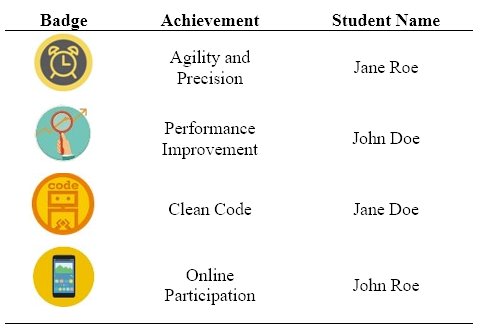
\includegraphics[width = 0.5\textwidth]{img/gamificationBadges.png}
    \caption{Examples of four badges in the SE course.}
    \label{fig:gamificationbadges}
\end{figure}


Leaderboard was incorporated with two resources: (i) a chart with partial grades and (ii) a Hall of Fame. The chart with partial grades was a digital document that was updated periodically and accessible in the course website, where students could track their grades and compare their performance against other students. To preserve the anonymity, the students were identified only by their university registration number. The “Hall of Fame”, on the other hand, is a special page in the course website that acknowledges the names of the top three best students of each course semester and the top ten students of all time. 

\begin{table}[htb]
\caption{Hall of Fame with the top ten students of all time in the SE Course}
\label{table:gamificationhalloffame}
\centering 
\newcolumntype{Y}{>{\centering\arraybackslash}X}
\scriptsize
\begin{tabularx}{.7\textwidth}{>{\hsize=.25\hsize}Y>{\hsize=.25\hsize}Y>{\hsize=.25\hsize}Y>{\hsize=.25\hsize}Y}
\hline
\textbf{Position} & \textbf{Grade} & \textbf{Semester} & \textbf{Student} \\
\hline
1                 & 96.50          & 2016-2            & Student A        \\
2                 & 93.70          & 2011-1            & Student B        \\
3                 & 93.50          & 2016-2            & Student C        \\
4                 & 91.55          & 2016-1            & Student D        \\
5                 & 91.25          & 2013-2            & Student E        \\
6                 & 90.75          & 2013-2            & Student F        \\
7                 & 87.04          & 2012-2            & Student G        \\
8                 & 86.79          & 2014-1            & Student H        \\
9                 & 86.50          & 2015-2            & Student I        \\
10                & 85.97          & 2014-1            & Student J        \\
\hline
\end{tabularx}
\end{table}

Table \ref{table:gamificationhalloffame} shows the Hall of Fame with the top-10 best grades of all time in the SE course. The second column of this table indicates the student grade in 100 points. The third and fourth columns indicate the semester and the student name, respectively. Although Figure 2 presents the best scores since 2012, this table was only made available in the second semester of 2016 based on historical data.

\section{Study settings}
\label{sec:gamificationstudysettings}

This section explains how we planned and executed this study. Section \ref{sec:gamificationgoals} presents the study goal and research questions while Section \ref{sec:gamificationmethod} discusses the research method we adopted. Section\ref{sec:gamificationsurvey} presents the survey and Section \ref{sec:gamificationinterview} explains the structure of an interview with 6 randomly selected students.

\subsection{Study Goals and Research Questions}
\label{sec:gamificationgoals}

The goal of this study is to investigate how the use of gamification could contribute to motivate students in Software Engineering education. To achieve this goal, we formulated two Research Questions (RQ) presented below.

\textbf{RQ1.} What are the student perceptions on the use of badges in the SE Course?

\textbf{RQ2.} What are the student perceptions on the use of leaderboards in the SE Course?

\subsection{Study Design and research methods}
\label{sec:gamificationmethod}

To answer the research questions, we adopted two techniques. First, we conducted a survey with the students to collect general impressions of the course (Phase I). Second, we conducted interviews to further understand the perception of the students about the gamification techniques used in the course (Phase II).

For both phases, the target population was all 36 students enrolled in the SE Course. They were invited to participate in both studies by e-mail. To reduce possible bias, one of the authors, who was not directly involved in the course execution, was responsible for the invitation of participants and data collection. The students were instructed that the participation in the survey and in the interviews was not compulsory and this participation did not provide any benefits in grades. Besides that, the student names were not revealed to the course instructors during the data analysis, to ensure that students would not be embarrassed for giving negative responses.

\subsection{Planning of the Study Phase I - Survey}
\label{sec:gamificationsurvey}

Survey is an empirical strategy for collecting information from or about people to describe, compare or explain their knowledge, attitudes, and behavior using questionnaire or checklist \citep{Pfleeger:2001}. In the first phase of our study, a survey was applied to collect a quantitative perspective of the students’ perception on the use of badges and leaderboards in the SE course. 

We created a questionnaire on Google Forms  with two parts: the first one was composed of 4 questions about the background of the students; the second part had 8 questions about the perception of the students about the gamification elements used in the course. Table \ref{table:gamificationsurvey} summarizes the items of the questionnaire. The background questions were named BQ1 to BQ4, while the questions of the second part of our survey were named SQ1 to SQ8. Tables \ref{table:gamificationsurvey} describes the possible answers for each question. Invitations were sent by e-mail to all 36 students formally enrolled in the course, as described in Section \ref{sec:gamificationmethod}.

\begin{table}[htb]
\caption{Questionnaire}
\label{table:gamificationsurvey}
\centering
\newcolumntype{Y}{>{\centering\arraybackslash}X}
\scriptsize
\begin{tabularx}{\textwidth}{>{\hsize=.05\hsize}Y>{\hsize=.45\hsize}X>{\hsize=.5\hsize}X}
\hline
\textbf{ID} & \textbf{Questions} & \textbf{Type of answer} \\ \hline
BQ1         & Are you familiar with the term “Gamification”?                                                                    & Likert Scale: \hfill \break (1) Definitely not; (2) Not; (3) Indifferent; (4) Yes; (5) Definitely yes                                    \\
BQ2         & How often do you play games?                                                                                      & Likert Scale:\hfill \break (1) Everyday; (2) Few times a week; (3) Few times a month; (4) Few times a year; (5) Never                             \\
BQ3         & Do you like playing games?                                                                                        & Likert Scale:\hfill \break (1) Definitely not; (2) Not; (3) Indifferent; (4) Yes; (5) Definitely yes                                               \\
BQ4         & If you play games, what are the main reasons you play games? (multiple options allowed)                           & Multiple Choices:\hfill \break  [ ] For skill development;\hfill \break [ ] For the challenges; \hfill\break [ ] For the fun; \hfill\break [ ] For the competition;\hfill\break  [ ] To enjoy spare time. \\
SQ1         & Did you find relevant the use badges to reward individual achievements of students during the course?             & Likert Scale:\hfill \break (1) Definitely not; (2) Not; (3) Indifferent; (4) Yes; (5) Definitely yes                                              \\
SQ2         & Did you feel motivated to perform better in order to be awarded a badge?                                          & Likert Scale:\hfill \break (1) Definitely not; (2) Not; (3) Indifferent; (4) Yes; (5) Definitely yes                                              \\
SQ3         & Would you like to see more badges for other achievements in this course?                                          & Likert Scale:\hfill \break (1) Definitely not; (2) Not; (3) Indifferent; (4) Yes; (5) Definitely yes                                              \\
SQ4         & Would you like to see the use of badges to reward individual achievements in other courses?                       & Likert Scale:\hfill \break (1) Definitely not; (2) Not; (3) Indifferent; (4) Yes; (5) Definitely yes                                              \\
SQ5         & Did you find relevant the use the “Hall of Fame” method?                                                          & Likert Scale:\hfill \break (1) Definitely not; (2) Not; (3) Indifferent; (4) Yes; (5) Definitely yes                                              \\
SQ6         & Did you feel motivated to improve your performance in the course due to the “Hall of Fame”?                       & Likert Scale:\hfill \break (1) Definitely not; (2) Not; (3) Indifferent; (4) Yes; (5) Definitely yes                                              \\
SQ7         & Would you like to see similar “Hall of Fame” method in other courses?                                             & Likert Scale:\hfill \break (1) Definitely not; (2) Not; (3) Indifferent; (4) Yes; (5) Definitely yes                                              \\
SQ8         & Do you have any suggestions or criticisms regarding the badges and “Hall of Fame” methods used during the course? & Open answer \\
\hline
\end{tabularx}
\end{table}

\subsection{Planning of the Study Phase II - Interviews}
\label{sec:gamificationinterview}

An interview is a research method defined by a conversation where questions are asked and answers are given \citep{Wohlin:2012}. In this study, we used interviews to compliment and deepen the results observed in the survey (Phase I), providing a qualitative perspective on the students’ perception of the gamification elements introduced in the SE Course.

As described in Section \ref{sec:gamificationmethod}, we sent invitation e-mails to all 36 students formally enrolled in the course. In the invitation email, we made it clear that the participant would have their personal data kept anonymously. We interviewed participants individually, face-to-face or by video-conference, as they prefer in order to make the situation more comfortable and natural for them. The interviews were executed after the conclusion of the course, and that the course instructor would not have access to the names of the participants, to reduce possible bias. Table \ref{table:gamificationinterview} describes the interview script. This script is composed of 9 questions, named IQ1 to IQ9. For instance, the first question (IQ1 in Table \ref{table:gamificationinterview}) asks students if they track their partial grades during the course.

\begin{table}[htb]
\caption{Interview script}
\label{table:gamificationinterview}
\centering 
\newcolumntype{Y}{>{\centering\arraybackslash}X}
\scriptsize
\begin{tabularx}{.7\textwidth}{>{\hsize=.1\hsize}Y>{\hsize=.9\hsize}X}
\hline
\textbf{ID} & \textbf{Questions}                                                                                                     \\
\hline
IQ1         & Did you follow up on your partial grades during the course?                                                            \\
IQ2         & Do you usually compare your grades in the course with the grades of your colleagues? Why?                              \\
IQ3         & What is your opinion about comparing your grades with the grades of your colleagues? Is it positive or negative? Why?  \\
IQ4         & Do you feel motivated to perform better when comparing your performance with other colleagues?                         \\
IQ5         & What did you think of the “Hall of Fame” feature to keep track of the top performers in the course in each semester?   \\
IQ6         & Did you receive any badge during the course? Do you think this kind of recognition of student achievement is relevant? \\
IQ7         & Did/would you feel motivated for receiving badges for your actions?                                                    \\
IQ8         & Do you believe that if the criteria for badges were known, would you work harder to obtain them?                       \\
IQ9         & Do you believe that there should be more badges during the course? Give examples of other kind of badges.              \\
\hline
\end{tabularx}
\end{table}

\section{Results}
\label{sec:gamificationresults}

In this section, we discuss the results of the study. Section \ref{sec:gamificationsurveyresults} presents the descriptive analysis of the results from the survey (Phase I). In Section \ref{sec:gamificationinterviewresults}, we discuss the qualitative results of the interviews (Phase II).

\subsection{Study Phase I - Survey Results}
\label{sec:gamificationsurveyresults}

From the 36 students in the SE course, 18 participants answered the survey. Of these students, 17 were undergraduate students of the Information System course and only 1 was an undergraduate student in the course of Computer Science. 

Figure \ref{fig:gamificationbq} presents the results for the background questions BQ1 to BQ3 regarding the background of the participants. The first question (BQ1) was about the participant familiarity with the term “gamification”. 11 participants (61.1\%) answered that they were familiar with this term (8 were somewhat familiar and 3 were definitely familiar). Only 4 participants (22.2\%) claimed that they were definitely not familiar with the term. Our second question (BQ2) was about the frequency in which participants play games. 6 participants (33.3\%) claimed that they play games every day, 4 participants (22.2\%) play few times a week and 5 participants (27.7\%) play sometimes a month. Only 3 participants (16.6\%) claimed they play games only few times a year. No participant claimed that never plays games. In the third question (BQ3), we inquired the participants about their appreciation for games. The results show that most of participants (13 – 72.2\%) confirmed that they like playing games.

\begin{figure}[!h]%th
\centering
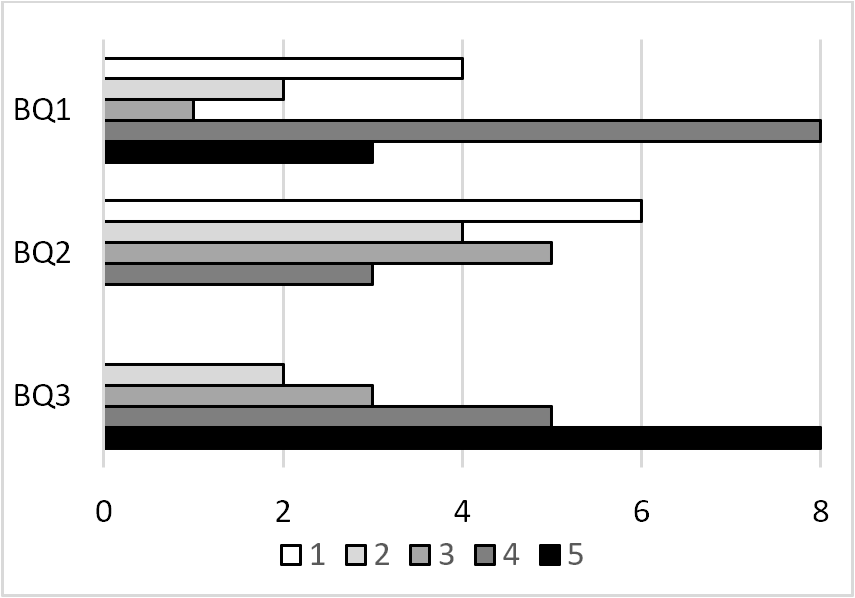
\includegraphics[width = 0.5\textwidth]{img/gamificationBQ.png}
\caption{Results for the survey background questions BQ1 to BQ3.}
\label{fig:gamificationbq}
\end{figure}

Figure \ref{fig:gamificationbq4} shows the results for the last background question (BQ4) in this pre-questionnaire. BQ4 aims to understand the reasons why the participants like playing games. In total, 17 participants (94.4\%) stated that they aim to have fun. In addition, 12 participants (66.6\%) claimed that one reason is to develop skills and the same number of students said they like to face challenges when play games. Less frequently, 11 participants (61.1\%) aimed to enjoy spare time and 8 participants (44.4\%) aimed for competition.

\begin{figure}[!h]%th
\centering
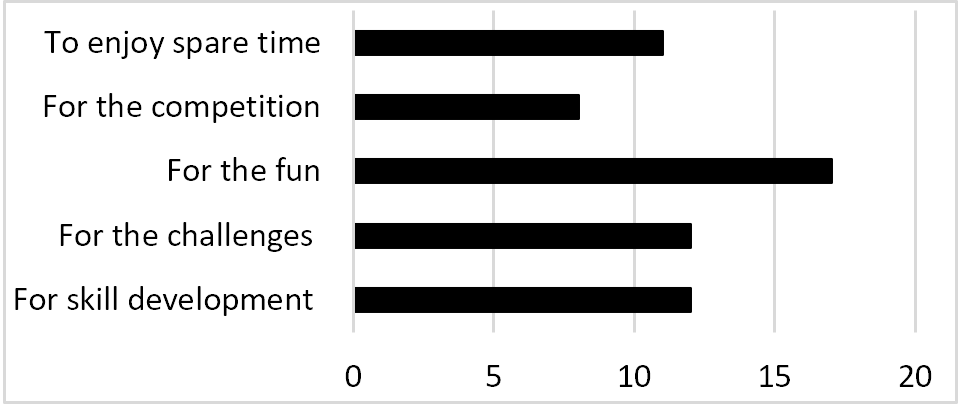
\includegraphics[width = 0.5\textwidth]{img/gamificationBQ4.png}
\caption{Results for the survey background question BQ4.}
\label{fig:gamificationbq4}
\end{figure}

Figure \ref{fig:gamificationsq14} presents the responses on the perception of students about the gamification elements introduced in the course. Questions SQ1 to SQ4 (described in Section IV-C) were defined to investigate the students’ perception on the implementation of badges in the course. 

As described in Section III, eight badges were implemented in the SE course. When asked if the participants found relevant the use of badges (SQ1), the responses were slightly positive (i.e., 7 positive, 6 neutral, and 5 negative responses as presented in Figure 3). However, when asked if these badges motivated them towards a better performance in the course (SQ2), Figure 3 shows that the responses were negative (9 negative, 5 neutral, and 4 positive responses). When asked if they would appreciate the existence of more badges in the course (SQ3), or the existence of similar resource in other courses (SQ4), the responses were positive in both cases. These data are indications that badges were well received by students, but they were not seen as a key factor of motivation by the majority of them. Further investigation about these results was explored in the interviews.

\begin{figure}[!h]%th
\centering
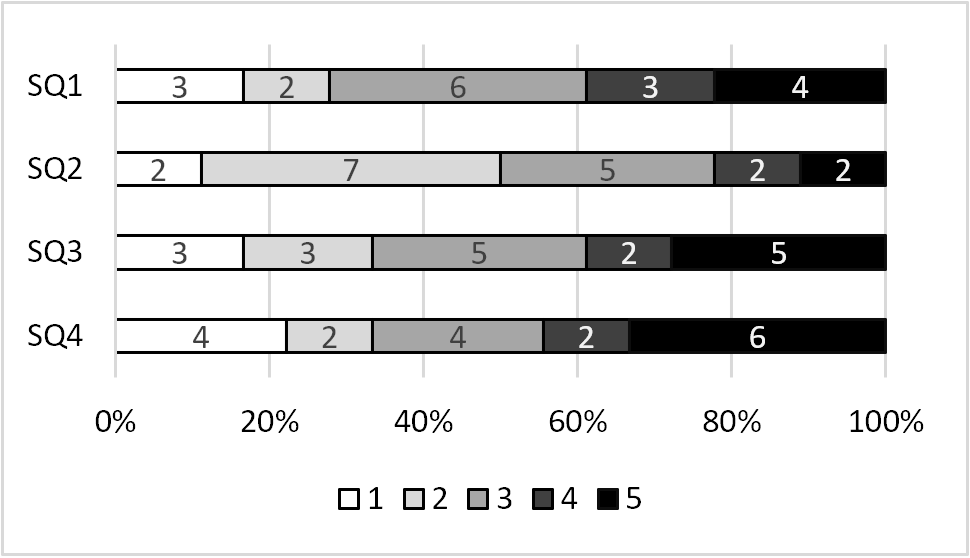
\includegraphics[width = 0.5\textwidth]{img/gamificationSQ14.png}
\caption{Survey results on the students perception on the use of badges.}
\label{fig:gamificationsq14}
\end{figure}

Regarding the leaderboards, specifically the “Hall of Fame”, the survey results were generally negative, as seen in Figure \ref{fig:gamificationsq57}. The questions SQ5 to SQ7 inquired participants about the relevance of such resource (SQ5), about how it motivated them to achieve better performance in the course (SQ6), and about the relevance of such resource in other courses (SQ7). Although there were very positive responses for the three questions, the negative responses were dominant. In the Phase II of this study, we investigated the reasons of such negative perception.

\begin{figure}[!h]%th
\centering
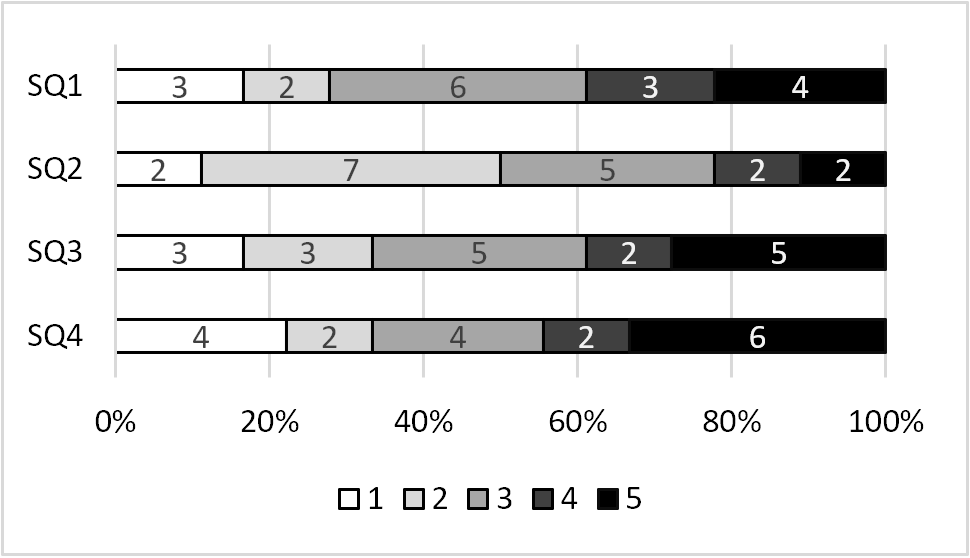
\includegraphics[width = 0.5\textwidth]{img/gamificationSQ14.png}
\caption{Survey results on the students perception of the “Hall of Fame”.}
\label{fig:gamificationsq57}
\end{figure}


Finally, we received 8 responses for the open question SQ8, regarding suggestions and criticism on the use of the game elements introduced in the SE course. Two participants suggested the addition of more badges as transcribed below.

“There should be more badges throughout the course”

“In general, I always work hard on the courses I'm enrolled. Thus, in the Software Engineering course I felt that my dedication was recognized. However, there should be more badges in the course for different types of activities in order to try to reach as many students as possible. In my opinion, the students who have also worked hard, but have not earned any badges, could be discouraged and feel that their effort was not recognized.”

Three participants suggested that badges could be converted to bonus grades:

It was not mentioned by the professor whether anyone who won badges or appeared in the 'Hall of Fame' would earn more grades for this. If I knew this could happen, I would be more motivated.”

“Badges could be converted into extra grades. In my opinion, perhaps it is the only way to really motivate students.”

“(…) Why there are no awards in grades? (…)”

Five students suggested that the course instructor should provide more details on how to obtain the badges, so students could pursue them actively:

“Maybe knowing what badges I could have obtained, it would make me motivated to "work" to get them. We did not have much incentive.”

 “I think if we knew the titles or how to get some badges, we could be more competitive to get them. Since we did not know which badges could be won, it was difficult to focus on something specific in order to earn them. It would be interesting to get at least some badges for the students in the next course. Of course, they could have some ‘extras’ grades. But if the students knew that it was possible to win the 'Clean Code' badges, for example, more students would try to make a better code. The proposal is super interesting.”

“It would be interesting to report about the badges, at the beginning of the course, so students could know about it in advance. And, what are the criteria for choosing the badges; it is also interesting to know. In this course, we had the badge 'Clean Code', for example, what would be 'Clean Code'? What are the specific characteristics the code should have, so that it is chosen? I believe that extra information would be interesting to add to knowledge for students who could not win the badges.”

“It would be interesting to disclosure the activities and rules to earn badges. Thus, we could work focusing on them since the beginning of the course.”

 “This method could be more interesting if the means of evaluation were clearer and more objective. As 'Online Participation', which online actions are rewarded? Log in every day at the platform (online course), or see all classes or post questions? In which case would any of these actions be more accounted than another? Is the ordering for better online participation updated every week? What do you get with your name in badge list or Hall of Fame? Are there awards in grades? Is it visibility among colleagues? And, is it the visibility among colleagues positive?”

\subsection{Study Phase II – Interviews Results}
\label{sec:gamificationinterviewresults}

Based on the results of the survey, we planned and conducted interviews to obtain a better understanding on the student perception on the gamification elements used. Six students accepted the invitation for interviews. The interviews followed the script described in Section \ref{sec:gamificationinterview}. In order to identify the interviewee responses, we adopt the identifiers “Participant A”, “Participant B”, “Participant C”, “Participant D”, “Participant E”, and “Participant F” to refer to the participants, while preserving their anonymity.

Regarding the leaderboards, we first investigated how students used the information about their progress that we provided. As described in Section III, the leaderboards were introduced in the course with two resources: (i) a chart with partial grades updated regularly, where students could compare their progress against other students; and (ii) a hall of fame. First, we investigated if the students kept track of their progress (IQ1) and if they used the partial grades to compare their performance against their colleagues (IQ2). Except for the Participant A, all participants stated they tracked their progress in the course. Moreover, all participants, except for the participant C stated they used the grade chart to compare their performance against their colleagues. Participant B, Participant D, Participant E, and Participant F stated that it was useful to understand the overall performance of the classmates in order to know what their real performance was. Participant A stated that this comparison was a consequence of the competitiveness in the classroom. However, Participant C claimed that he always tried to achieve the best grades, and it was not interested in comparing their performance to the others.

Regarding the positive aspects of this comparison (IQ3), we observed three main positive feedbacks: (i) students with lower performance than the average performance of the class would feel motivated to perform better, (ii) students try to understand how they could improve their learning strategy, and (iii) they talk to classmates with better performance to exchange knowledge. One possible issue pointed by the participants was the risk of students acting only in response to the general performance of the class, i.e., if everyone is getting poor grades, there is no reason to try to perform better. Participant D also warned about the risk of creating ego conflicts in the class. With respect to motivation of improving because of this comparison (IQ4), only Participant A and Participant D had negative responses. Participant A would only feel inclined to try to perform better in case the class has a better performance in general.
Question IQ5 inquired the participants about their opinion on the “Hall of Fame” resource. Participant A did not like the strategy to implement the Hall of Fame, and claimed that it did not capture the essence of Software Engineering, and it would be better to acknowledge other aspects such as the best product developed instead of grades. The other participants had positive perceptions about the recognition provided by the Hall of Fame.

From the six participants in this study phase, only one (Participant C) received badges (two) during the course. Participant C found the experience positive and rewarding. Even without receiving badges, Participant B, Participant D, and Participant F found this element rewarding and benefic as a form of recognition for specific actions. Except for Participant A, all others responded question IQ7 positively.

When we asked participants about the strategy of not revealing the criteria for receiving each badge, the opinions were mixed. Participants B, C, and E defended the idea of specifying the criteria for each badge as soon as possible, because students would establish additional goals besides the grades and, from an educational perspective, it would become an opportunity to pay attention to aspects that they would not normally observe. For Participants C, D, F, the criteria for obtaining badges could make students focus too much attention on the game aspect and, somehow, they could have a counterproductive effect on learning. Except for Participant A, all students were positive when asked if they would like to see more badges in the course.

\section{Discussion}
\label{sec:gamificationdiscussion}

This section discusses the results presented in Section \ref{sec:gamificationresults} and our general findings regarding the research questions defined in Section \ref{sec:gamificationgoals}.

\subsection{Badges in a Software Engineering course (RQ1)}
\label{sec:gamificationdiscussionrq1}

Our results showed a general positive perception of the students towards the use of badges during the course. Considering that we did not explore this resource to the full potential, by having only eight badges, the students showed interest on them.

Student perception on the role of badges was twofold: (i) they served as a social reward, a public recognition of the student skill or effort; and (ii) they served as a secondary goal, besides the grades and approval, to strive for when performing the course activities. These two elements can be further explored to motivate students not only in performing better in the course, but also as a motivation to further explore Software Engineering good practices. For instance, it can make students aware of good practices related to the use of tools, of good practices for coding, and so on. In this initial study, we opted for keeping the requirements for earning badges in secret to avoid the students expectative of grades, but we are aware of the motivation it can generate.

One of the students participating in the interviews was particularly unsatisfied about the gamification elements in the course, because he wanted they to explore the practical nature of Software Engineering and professional practices. This is an important feedback, considering that another approach would be the gamification of specific SE activities, as discussed in Chapter \ref{ch:sms}.

Another issue we observed about the gamification strategy is that most students think of grades as the only reward they can achieve in a course. The feedback received in the survey reflects this rationale: students often asked how the badges would translate into higher grades. It was a surprise to see that they also perceived some value in the social recognition aspect of badges.

\subsection{Leaderboards in a Software Engineering course (RQ2)}
\label{sec:gamificationdiscussionrq2}

The use of leaderboards in the course was received with mixed opinions. The results of the Phase I of the study had more negative responses than positive ones. In the survey, we focused specifically in the Hall of Fame resource. The results obtained from Phase II had given us additional perspectives on this issue.

First, we observed that students used the partial results to regularly compare their performance against each other, and felt motivated to perform better when they had lower grades than the others. These periodic updates were seen as a baseline to understanding the overall performance of the class and to assess their own performance. The interviews showed that the Hall of Fame was seen as a social recognition of the efforts of the students, and it was also seen in a good light from this perspective. We believe that the negative aspect of this strategy may be related to the exclusive focus on grades. While grades are a direct measure of the student performance in the course, it could be complemented by other measures. For instance, we could use additional badges to assess the student performance by their number of achievements.

\section{Threats to validity}
\label{sec:gamificationthreats}

In this section, we document potential threats to the study validity and discuss some bias that may have affected the study results. We also explain our actions to mitigate them.

\textbf{Results:} The results presented in the study are first and foremost observations, suggestions and lessons learned for further research. We have obviously presented our own view of the analysis of the surveys and interviews. However, there may be several other important issues in the data collected, not yet discovered or reported by us. 

\textbf{Interviews:} In order to avoid the risk of bias and misinterpretations of the six interviews in our study (and also to avoid depending on good memory of interviewers), we decided carefully to record all interviews and shared with another researcher of this study. After that, one of them was responsible for transcription of all interviews. Therefore, audio and text were available for analyses. Moreover, some meetings were necessary in which the researchers discussed about each answer and extracted all positive and negative impressions about each question. Thereby, we could increase the chance of obtain an unbiased interview analysis.

\textbf{Number of Participants:} The data collected only capture the subjective opinion of each student. A larger number of participants should be interviewed to capture the general view of a broader audience. However, it was our first experience with gamification on software engineering education, and we had a good number of volunteers to participate in our study, without any concrete benefits (i.e., grades). About 50\% of all students of the course participated in the survey, but less than 20\% took part in the interviews. However, we do not attempt to generalize to a larger population, but merely to discuss some interesting issues discovered during this study (survey and interview). We then presented some discussions, suggestions, lessons learned, and insights for future research. Additionally, this study is an experience report. Therefore, we are concerned in reporting our observations in this scenario, rather than validating any hypothesis.

\section{Final Remarks}
\label{sec:gamificationfinal}

In this chapter, we described an experience of introducing gamification elements (namely, badges and leaderboards) in a Software Engineering course. We are aware that the gamification technique has more to offer, but in this first experience, we relayed on the most basic and popular elements. Our experiment was focused on the student perception and the motivational aspect of the approach, rather than on their impact in grades.

Our results showed a positive perception of the use of badges in the course. Students showed interest in badges and saw them as both (i) a social reward and (ii) secondary objectives to strive for in the course, besides grades and the approval. Regarding the use of leaderboards, our quantitative results showed a negative perception of the resource. However, interviews showed that students like to compare their performance against each other, and, when their performance is lower than the rest of the class, they feel motivated to try to perform better or to rethink their learning strategy. In addition, students liked the possibility of being recognized for their efforts.

We believe that gamification has a motivational role in Software Engineering education that requires  further exploration and evaluation. Although our results cannot be generalized, we provided evidences on the relevance of this technique in an educational environment. A major drawback is that gamification requires significant effort from instructors to setup and to maintain their elements during a course. Significant lessons learned from this study are:

\begin{itemize}
    \item Social recognition is relevant for students motivation. However, grades are still the most common reward they expect;
    \item Badges were perceived as secondary goals for student to strive for in addition to approval in the course. Therefore, it is relevant to evaluate the role of badges as motivators for the adoption of specific SE skills, such as following a process. 
    \item One student explicitly claimed that the Gamification should promote the practical aspect of SE education. However, as a first contact with gamification we opted for a more simplistic approach, that was positively received.
    \item The Hall of Fame (leaderboard) was received with mixed opinions. While the students would not compare their grades with other students for the purpose of competition, they compare grades with the purpose of assessing their performance in the course in comparison with their colleagues.
    \item Students would like the existence of more badges and that everyone could try to earn them, instead of having badges awarded for a single student. Again, it is an indication that students are more interested in personal progress than competing with colleagues.
    
\end{itemize}

Additional details on the results of this study can be found in \cite{Souza:2017}.

\chapter{The experience of using Project-based Learning in Software Engineering Education}
\label{ch:actionResearch}

This chapter describes the experience of adopting Project-based Learning (PBL) in an introductory software engineering course at Federal University of Minas Gerais (UFLA). The goal was to introduce a practical approach to allow students to experience software development process. However, there were many challenges observed in setting up and conducting the course with this learning method. Therefore, the goal of this study is to summarize the lessons learned from the adoption of PBL in software engineering education, in terms of challenges observed and the perceptions of the students regarding the course. To achieve this goal, an Action Research study was carried in four academic periods of the Software Engineering course offered in the curriculum of the undergaduate program in Information Systems at UFLA.

The remainder of this chapter is organized as follows.

\section{Study settings}

This section explains how we planned and executed this study. Section III-A presents the goal and research questions of this study. Section III-B discusses the research strategy to answer the research question. Section III-C describes the process and result of the primary studies selection. 

\subsection{Study Goals and Research Questions}

The goal of this study is to understand the challenges and lessons learned from the use of Project-based learning in Software Engineering Education. To achieve this goal, we propose the following Research Questions (RQ):

\textbf{RQ1.} What are the challenges of using PBL in an introductory software engineering course?

\textbf{RQ2.} What is the perception of students on the use of PBL in an introductory software engineering course?

\subsection{Research method}

To answer the research questions, we conducted an Action-Research study in an introductory Software Engineering course with the purpose of incrementally refining a PBL approach to introduce a practice-oriented learning method.

Action Research is a research approach that advocates the intervention in a problem, the proposal of solutions and their application, for purpose of solving the problem and creating theory regarding the action (Coughlan and Coughlan, 2012). In Action Research, the researchers attempt to solve a real-world problem while simultaneously studying the experience of solving the problem (Davison et al., 2004). While most empirical research methods have researchers attempting to observe the world as it currently exists, in Action Research, the researchers aim to intervene in the studied situations for the explicit purpose of improving the situation (Easterbrook, 2008). 

According to Easterbrook (2008), Action Research has been pioneered in fields such as education, where major changes in educational strategies cannot be studied without implementing them, and where implementation implies a long-term commitment, because the effects may take years to emerge. Similarly, Santos and Travassos (2009) suggest that this method seems to be a useful research methodology when considering the social challenges involved in SE research, and the long history of success in similar domains, in terms of research practice and challenges, such as education and nursing.

\subsection{Study design}

In Action Research, activities are organized in a structured cyclic process, called “Action Research Cycle”.  This process usually includes the following activities: “Diagnosis”, “Planning”, “Intervention”, “Evaluation”, and “Reflection and Learning” (Davison et al., 2004). Figure 1 presents the Action Research Cycle adopted in this study. 

Figure 1. Action Research cycle, adapted from Davison et al. (2004)

The study was carried in four iterations of an introductory Software Engineering course, from 2016 to 2017. Each course is considered an iteration of the Action Research cycle. In each cycle, we executed the following activities in each phase:

\textbf{Diagnosis and Planning Phase:} Prioritization of problems to address in the current cycle and definition of actions to be taken. This phase was executed before the beginning of each course, defining a Course Plan describing how the actions would be translated to teaching strategy;

\textbf{Intervention Phase:} Execution of the Course Plan and data collection. During this phase, we assigned, monitored, and assessed Practical Projects.

\textbf{Evaluation Phase:} Evaluation of the course outcomes, from the perspective of students and instructors. In this phase, we analyzed the data collected during the course.

\textbf{Reflection and Learning Phase:} Identification and documentation of lessons learned. During this phase, we reflect on the outcomes of the cycle, identifying positive outcomes from the actions taken in the current cycle, and possible issues to be addressed in following iterations.

\subsection{The introductory software engineering course at UFLA}

The Software Engineering course (“SE course”, henceforth) is a 60 hours introductory course offered every semester at Federal University of Lavras, included in the curriculum of the Information System Bachelor undergraduate program. The SE course aims to introduce students to the concepts and methods required for the development of large software intensive systems. The prerequisite for taking this course is the approval in the Object-oriented Programming course.

This Software Engineering course is mainly based on two textbooks: Software Engineering by Sommerville [14] and The UML User Guide by Booch, Rumbaugh, Jacobson [15]. The course syllabus includes: software development process, agile methods, software requirements analysis and specification, software design, system implementation and testing, configuration management, and software quality.

\section{PBL in the SE course}

This section reports the execution of the Action-Research. For this study, we considered four iterations of the SE course. In the following subsections, we describe how Project-based Learning was adapted in each semester. Table I presents the four iterations, identified by an id (class), the number of students, the type of project used and the distribution of teams, and the data collection strategy (evaluation instruments)  

TABLE I. SAMPLES

In the evaluation phase of each Action-Research cycle, we briefly discuss the results of the questionnaires. The complete analysis of this evaluation instrument is presented in Section IV.

\subsection{Class 2016.1}

In the Planning Phase of the first iteration of this study, we defined the following problem: “How to introduce Practical Software Projects in an introductory SE course, to provide students with practice?”

Initially, we planned the use of a real project with real clients. The selected project was a Web system to manage the allocation of rooms for classes at UFLA and their keys. The clients were employees at DADP (Pedagogical Support and Development Office), the sector responsible for the reservation of physical spaces and for providing resources (e.g.: datashow) and keys to access the requested rooms.

Thirteen students enrolled in the course. Given the small number of students in the course, we opted to allow all students to work together in a single project. The class was planned having an evenly distribution of lectures in the classroom and in the laboratory. However, the theory would always be provided in accordance to the evolution of the software project, and using the project as a driving problem to motivate learning.

To achieve the learning goals of the course, in the execution of their project, the students would have to:

-	Elicit the customer requirements

-	Describe the system requirements as functional and non-functional requirements

-	Analyze the software behavior using appropriate notations (e.g.: use case scenarios)

-	Discuss and plan the software design

-	Select appropriate technology to develop the software

-	Construct the software in accordance with specifications

-	Test the software

-	Manage software development using appropriate project management tools

-	Use appropriate tools to manage software configuration

-	Use agile methods

The project corresponded to 55% of the course grade, divided in individual (15%) and team (40%) evaluation. Additionally, there would be a written exam (25%) and activities in class (20%) for individual assessment.
During the course (Intervention Phase), students organized themselves in sub teams: a requirement team, a development team, and a test team. The first classes were devoted to introducing Software Engineering, Software Process and agile methods. The students were instructed about the project they were going to develop, and how they would adapt the Scrum framework to organize their development iterations. The project was organized in three iterations. In each iteration there was a class devoted students presentation of what they did in the iteration (similar to a Sprint Review event) and to plan the goals of the next iteration (similar to a Sprint Planning event).

In the first project iteration, students met with the customer and collected his needs in an interview, supported by the professor. Then, students detailed the requirements, designed use cases diagrams and documented use cases scenarios, and created user interface prototypes. Finally, they arranged a second meeting with the customer for validating and prioritizing the requirements, or negotiating possible changes.

In the second iteration, students investigated and discussed possible technologies (languages, frameworks, database systems) they could use to implement the software. Students presented seminars in classroom to disseminate their findings and they collaboratively selected XXXXXXXXXX. Then they discussed the software design and devoted the rest of the second and third iterations to developing and testing the software.
Regarding the use of management tools, the students had to identify and apply a project management tool in their project. They used “Asana” to plan and monitor their activities. Similarly, students had to use Git and GitHub for controlling the evolution of their software.

To support student activities, the professor conducted classroom activities, mentoring students. For instance, a class was devoted to explaining the purpose and how to develop user cases diagrams and scenarios, using the project as a case. The goal was to use classroom time to support students in developing work products they could use in their projects. In these activities, students were individually evaluated to ensure that, even if they organize themselves as sub teams for the execution of the project, each of them would still experience the hands-on practice. These exercises corresponded to 20% of the total grade.

The end of each iteration resulted in a seminar where students presented the results of that cycle, and planned the next, following the structure of the scrum events “Sprint Review”, “Sprint Retrospective”, and “Sprint planning”, respectively. The final release would be presented to the customer, however (i) the responsibility of handling the keys and resources for the physical spaces was relocated from the original customer to another department at UFLA, and (ii) the customer was not available for attending the class. It frustrated  the students expectations. 

Finally, a final written exam was composed of questions about theory contextualized in the case of the project they developed, to evaluate the students understanding about the concepts covered in the course.
In the Evaluation Phase, we observed that the project was satisfactory. The students were able to develop a functional application in accordance to the customer needs, while practicing the software development life cycle. However, there were some shortcomings in the overall result:

-	Following the open-ended nature of the canonical PBL approach, the project was loosely structured. Therefore, the evaluation of students was subjective, focusing on the correctness of the work products they developed, and the individual contribution observed in classroom. 

-	The lack of clear evaluation criteria made the students confuse about how they would be evaluated. 

-	The version control tool (Git and GitHub) was underused. Only one student used the tool, as he was responsible for integrating the source code provided by his teammates locally. Therefore, the course failed to showcase version control software as a collaboration tool.

-	Big team: The large size of the group encouraged students to create sub teams. It created communication problems between the sub teams, and it lead to problems in work products consistency. Additionally, the distribution of effort was unbalanced, as some students worked more than others, and it was difficult for the professor to objectively assess the individual participation of students. Finally, there was the risk of not having students experiencing all stages of the project execution.

-	Real Customer: The use of a real project, with a real customer, motivated students. However, the customer was not always available. In the middle of the project, the responsibility over keys and resources for classroom was moved from the original customer to another department ant the institution. Therefore, the use of real clients can be risky, because it introduces variables that are out of the instructors control.

-	Lack of instruments to collect student feedback.

\subsection{Class 2016.2}

In the Planning Phase of the this Action Research cycle, the following changes were introduced:
Type of project: We decided to allow students to choose their own projects. Therefore, instead of having an requirement elicitation activity with a customer, the students were required to create a “Product Vision” document, providing an overview of the scope of the project (objective, main features, and restrictions). 

\textbf{Team size:} given the number of students enrolled, we limited the size of teams to 5 students, to avoid the problems related to the size of the team observed in the previous semester.

\textbf{Clear objectives and evaluation criteria:} We defined a list of work products the students were expected to produce, and a checklist of attributes we would use to evaluate those work products. This decision was made to provide clear evaluation criteria both for instructors and for students.

\textbf{Use of Git:} we specified the task of documenting releases using Git (using “Tag” feature), and we assigned an activity for students to create a tutorial video for Git. This assignment took the form of a contest, with the best video being awarded with 5% extra grade.

\textbf{Course evaluation questionnaire:} A questionnaire was planned to collect data on the students perception of the course.

Table II. X

During the course (Intervention Phase), students followed a similar development cycle from the previous semester, with three development iterations similar to Scrum Sprints. They formed five teams. Given the change in the type of project, the first project iteration was devoted to negotiating the scope of student’s projects. The list of projects they chose to implement is described in Table X. However, this negotiation consumed considerable time, because each team had to reach consensus on what they wanted to do, and the professor had to approve that scope, considering a minimum complexity expected. For instance, Team B initially wanted to develop a simple website. The instructors had to intervene and assist them in choosing relevant features to transform the project in a Web application with more opportunity to apply software engineering concepts. 

Table III. Students Projects for class 2016.2

In the second project iteration, team C decided to change their project scope to an entirely different application. Therefore, they had a substantial effort recreating the Product Vision, Requirements, and Project Plan documentation. The change was done because one of the team members quit the course, and this particular student was leading the project, and the other students had little knowledge on the original business domain. 

The classroom activities were difficult to manage, because of the multiple projects. The goal of these activities were to provide mentoring for students to apply the concepts learned in lectures in their projects, and to promote discussion and share of knowledge. Consequently, students had difficulty in sharing lessons with other teams and discussing about the techniques they had to apply in their projects abstracting different project scopes. For the instructors, it was also difficult to provide meaningful examples because it was required to cover all students’ projects.

To support the use of Git, we assigned an activity for students to create a video tutorial for the tool. The best video would be awarded with 5\% extra grade. The assignment was received with great enthusiasm, and all teams produced high quality tutorials. The contest aspect kept students motivated. However, the same engagement was not reflected in the use of Git in the development of the project. Even having specific evaluation criteria related to the use of the tool, the teams did not incorporate the tool in their development activities.

By the end of the course, all teams were successful in developing their products. However, we observed that some teams created documentations that did not reflect the activities they performed in their projects. In some cases, instead of documenting their decisions and what they did in the project, students opted to use templates found in the internet that were much more complex than what they were expected to deliver. 
Therefore, the evaluation criteria may have led students to believe they would be evaluated for the quality of the documents they produced rather than the activities they performed to produce those artifacts. Additionally, students only delivered their work products in the exact date of the deadlines. Therefore, it was difficult to provide guidance and feedback to avoid this problem in advance.

In this class, we applied a questionnaire at the end of the course to collect data on the students’ perceptions of the course. The detailed description and analysis of the questionnaire is described in Section V. For the purpose of evaluating the course in the Action Research study, we consider the questions regarding: (i) how much the project contributed to their learning experience in the topics of Software Requirements, Software Design, Software Construction and Implementation, Software Construction, Configuration Management, and Agile methods; (ii) what are positive aspects of the software project in the course; (iii) what are negative aspects of the software project in the course; and (iv) additional commentary on the course.

Figures X and Y present the students responses about their perception on the impact the project had in learning the topics covered in class. The results were mostly positives, with a better response rate for the topics of “Software Requirements”, “Software Design”, and “Agile Methods”.

Figures

The positive aspects pointed by the students included: (i) the project contributes to a better understanding of the topics learned; (ii) the project allows students to practice the theory learned; (iii) the project allows students to develop teamwork skills; and (iv) the simulation of the professional environment. Some quotes from students:

“The project permitted the topics of the course to be retained and understood much better”
“Better understanding of the learning topics, better interaction in the work team, and experiencing the topics learned in practice”

“The project is a good simulation of what happens in a company (teamwork, customer relationship, processes to be concluded in deadlines, product development, documentation, and others).”
The main negative aspects pointed by the students were (i) the time-consuming nature of the practical assignment, and (ii) the lack of commitment of team members. Some quotes of the students:

“There are people in the team who do not contribute in anything”

“It demands a considerable amount of time”

“The lack of time to conciliate the project with the remaining activities in the university”

The following lessons were observed as shortcomings in this cycle:

\textbf{Students projects:} Allowing students to choose their projects consume time as they try to reach consensus with their teammates. Additionally, students change their scope during the project execution, as they try to reduce its complexity in order to make it viable. One of the teams (Team C) decided to change their project in the second iteration, and they had substantial rework with the specification. There was the risk of unbalanced projects complexity.

\textbf{Different projects:} It is harder to promote discussion among students when they are considering different projects as their references. It is also harder for the professor to mentor students in classroom activities when each team is working in different contexts. It would require more teaching assistants to support a higher number of different projects.

\textbf{Too much focus on documentation:} By providing students with evaluation criteria based on the artifacts they have to deliver, students focused more on the documentation than on the execution of activities and their purpose. For some teams, the software they were developing did not correspond to the documentation they produced, therefore they were creating documents with little value.

\subsection{Class 2017.1}

For this Action Research cycle, only seven students enrolled in the course. Considering the issues faced in the previous semester, the following changes were introduced in the Planning Phase:
Type of project and customer: Considering the problems with multiple projects in the previous semester, it was decided to have a single project. To increase the instructors control over the project, it was decided to use a fictitious project, where one of the instructors (the teaching assistant) played the role of customer. The project for the semester was an Web application for managing a hostel.

Team composition: Given the low number of students enrolled in the course (only 7), we opted for a single team.

Project Activities and evaluation criteria: In this semester, in the beginning of each Sprint, the Professor would act as a coach, describing and negotiating the goals of the sprint, and the outcomes students were expected to achieve. Students were free to choose how to document the outcomes of each activity. The evaluation rubric was composed 

Focus on competences rather than on artifacts: We adopted SWECOM [ref] as a reference to plan the learning outcomes of the project. Therefore, all activities planned for the project execution, should be grounded in the skill sets and activities from this model. However, this model was transparent for students, to avoid any confusion. Therefore, the Professor was responsible for identifying the skills sets and activities from SWECOM that were relevant and compatible with the course syllabus.

Student self-assessment form: By the end of the course, the students would have to fill a form, based on the skill sets and activities selected from SWECOM. The goal was for students to reflect what activities from the model they believed they performed individually, and how it was executed in their project. Therefore, we could evaluate the perception of the students on the development of competences, individually.

In the first project iteration (Intervention Phase), the professor negotiated that students had to: (i) understand the scope of the project, (ii) investigate the technologies they would use to implement the software, (iii) plan how to manage the software development.

The students performed an interview with the instructor, who played the role of customer, to identify the customer requirements, they produced system requirements, user case diagrams and scenarios, and prototypes. All activities were supported by the instructors with classroom activities and short lectures where the students were mentored on what they had to do. For the technologies for the development of the project, they decided to use XXX. For the management of the project development, students decided to use Trello. GitHub as the platform for version control, was the only mandatory tool. The development iteration was concluded with the validation of the requirements with the customer, where students presented a seminar. They named their Project “My-Spot”.

In the second development iteration, the professor negotiated the expected features for the first software release, and the following outcomes: the high-level architecture of the system, the use of the selected tool to manage the development progress, the use of Git, development of test cases for the application. In the end of the iteration, students presented their results for the professor, and validated the features of the first software release. During the validation, the instructor playing the role of customer tested the application, and requested a requirement change in the project.

In the third development iteration, the professor negotiated more features for the next software increment, and the following outcomes: review and update their specifications and design according to the project evolution, create new test cases and develop unit tests.

The results of this class were positive regarding the professor expectations: students produced a software product according to customer specification and applied what they learned in classroom in their process. The feedback from students was also positive. Figures X and Y present the students responses about their perception on the impact the project had in the learning of the topics covered in class.

Figures

The positive aspects pointed by the students were: (i) the simulation of the professional environment, (ii) the possibility to practice the theory learned, and the (iii) the requirement elicitation process. Some quotes of the students:

“The notion, even if it is minimum, about each one of the processes, artifacts and people in the project development.”

“It allows the student to develop the ability to see and experience in practice the theoretical concepts presented in classroom. It allows the identification of fundamental variables for the execution of a software development project, which only theory would not cover.”

“The software elicitation was very interesting”

“The fidelity to the (professional) market and the context in which software engineering is applied in practice”

The negative aspects were related to the (i) time-consuming nature of the practical assignment, (ii) the belief that programming is a deviation from the scope of the course, and (iii) the lack of depth in each stage of software development process. Some quotes of the students:

“A negative aspect was time. However, not considering the deadlines for projects deliveries, but the lack of availability of team members to execute all activities”

“The necessity of time available for students regarding tasks that are not fully connected to the course 
content, such as the product development.”

“The lack of possibility to act and to get deeper in each of the processes and roles of the development model (scrum). The ideal would be to be able to go through each of the areas in an in-depth way to better understand the pains of each area to propose improvements and better understand the processes.”

Lessons:

-	Type of project and customer: This change solved a number of issues of the previous courses: (i) Less time consumed negotiating the scope of projects; (ii) increased availability of the customer, therefore the students had more contact with a stakeholder; (iii) higher immersion of students in a simulated work environment; (iv) more control over the project, for instance we could simulate changes in the scope after each sprint review.

-	Project Activities and evaluation criteria: students had a more active role in negotiating their learning goals. Consequently, students invested more in the activities. For instance, the use of Git increased considerably, the students explored the use of branches, 5 students acted as active collaborators in the Git project, and they reached the mark of 60 commits. After the second sprint, the students felt the necessity of refactoring the code to increase maintenability. They changed from a perspective of documenting first, to a perspective of discussing possibilities, experimenting and then documenting what was relevant.

-	Team composition: The low number of students allowed the instructors to offer more mentoring. Therefore, it was easier to guide and to monitor the individual  progress of students.

-	Activities in classroom: Considering that there was only one project for the class, it was easier to devote classroom activities focused in providing mentoring for the development of the software project. All activities in classroom were based on the theme of the project. Therefore, all activities in classroom contributed directly to the development of work products students could use in their project. 

\subsection{Class 2017.2}

The goal of this semester, was to reproduce the experience of the previous class. However, in this class, the number of students increased from 7 to 11. Therefore, in the Planning Phase, the following decisions were taken:

-	Gamification: introduction of game elements and mechanics with the purpose of increasing students focus on performing the activities, without the constant observation of the instructors. We used the rationale of appraisal methods from maturity models standards such as SCAMPI and SPICE. Based on a set of competences from SWECOM, we defined a list of achievements. Students had to claim achievements, providing relevant evidences to justify their request. During sprint reviews, the instructors interviewed the team to confirm that the practice related to the achievement was understood. The students grade was equivalent to the number of achievements obtained. Table X presents the game elements used in the course.

-	Type of project and customer: Similar to the previous semester, an instructor played the role of the customer. However, instead of a fictitious project, the class had to develop a Web application to assist the management of a very small factory in the cleaning material business. The instructors visited the factory and interviewed the managers and employees to understand the problems and how a software could help managing the factory operation. Therefore, the students would work in a real problem, with a simulated customer.

-	Team composition: There were 11 students enrolled in the course, therefore they formed two groups of 5 and 6 students. This decision was made to avoid the problems observed in the 2016-1 class related to the size of the group. Both groups would now conduct their own project, sharing the same theme. 

Table IV. Game elements introduced in Class 2017.2

In the beginning of the course (Intervention Phase), students were presented with “game rules”, they organized themselves in teams, and each team chose the name of their fictitious software company. The two teams were named “14A Solutions” and “CALFV”. At the start of each Sprint, the teams were provided with a list of achievements and badges available for the Sprint. In each Sprint, there were 9 badges available. To obtain each badge, the teams had to earn 1-3 specific achievements. Therefore, there was a total of 27 badges and 74 achievements. There were some achievements that were cumulative, e.g.: there were three achievements related to describing 4, 8 and 12 user cases scenarios, respectively.

For instance, in the second sprint, the badge “Project Manager” was available, and to earn this badge, the following achievements were required: “Use a management tool”, “monitor the progress of the sprint”, “identify and treat deviations”. Both teams earned this badge. For the first achievement, both teams used the tool “Trello” to manage the sprint activities, and added the instructors to their boards, as evidences of use.  For the second, one the teams provided screenshots from their boards from one week to the other. For the third …

One of the teams (“CALFV”) immersed more in the scenario and created a spreadsheet to actively plan and document the evidences for each achievement. This team also made more questions about the achievements and how to obtain them. As a result, they earned more achievements (58 out of 74 – 78,4\%) and badges (18 out of 27 – 66,7\%). Consequently, their grade in the assignment was higher. The other team (14A Solutions) only provided evidences at the deadlines. Therefore, they made little use of feedbacks. This team earned a considerable number of individual achievements (43 out of 74 – 58,1\%), however, the number of badges was very low (11 out of 27 – 40,7\%). By the end of the course, both teams successfully delivered two functional increments of the software. However, one of the teams performed better regarding the process.

The questionnaire results presented positive results regarding the contribution of the students in learning and developing skills in the five topics. Figure X and Figure Y show that, following the pattern of the previous classes, “Software Requirement” had the most positive responses (“4 – Substantially” and “5 – Totally”).  In this course, “Software Design and Modelling” had the second best responses, the remaining topics were balanced.

Figures

Regarding the positive aspects, students mentioned the opportunity to experience an environment similar to the professional, the possibility to practice the theory they learned, and exercising teamwork skills. Some quotes of the students:

“(the project) demonstrates how Software Engineering is totally connected with the professional market, and it prepare us for this future.”

“(the positive aspect is) the simulation of a real development, because it allows us to have a professional and correct perspective for good software development.”

“It introduces the reality of software development in industry in a more tangible way.”

“It helps in familiarizing with the subject, forcing us  to learn and to practice what was taught during the classes.”

“Having a more practical perspective about the area (Software Engineering) rather than only theoretical.”

“hands-on helps developing skills.”

Most of the negatives aspects pointed by the students are related to the time-consuming nature of the project, and the recurring problems of team members who believe their peers did not collaborated equally:

“(there was) little time to execute it (the project) along with many other parallel activities.”

“the development of the whole project in a short time is complicated”

“some lack of commitment from some team members”

“in the end, only one member of the team perform all the work related to the software development, because the others are not interested”

From this course, the lessons learned were:

-	Project based in a real problem: …

-	Use of Gamification: The use of game elements to drive the PBL course was satisfactory. The main contribution was providing students with a structured set of activities, and giving freedom for students to choose how and when to address each one. The idea of having to provide evidences to earn achievements, reinforced the reflection on what they were doing. The feedback mechanic also contributed to a higher involvement of the students of one team, who contacted instructors more often to question about the correctness of their evidences. This also allowed the instructors to observe a continuous effort from this team. The teams were more immersed in the shared goal to obtain the reward, than in the competition among teams.

-	Having the same project for all teams contributed for the activities in classroom, where the students could share experiences in a common context. Although there was the risk of students copying the work of others, it did not happen. The teams developed their projects in different technologies, and each team produced different types of documentation. We believe the focus on the activities, rather than the deliverables, contributed to this outcome.

\section{Questionnaire analysis}

In this section we analyze the results of the questionnaires applied in three classes discussed in the previous section (2016-2, 2017-1, 2017-2). The questionnaire was structured in five sections, and eleven questions. The Questionnaire structure is presented in Table IV.

Table V. Questionnaire structure

\subsection{Population sample}

A total of 36 students were formally enrolled and did not evade the courses. The students were invited to participate in the study in the last day of each course. In order to avoid possible bias in their responses, they were informed that the participation in the study was not mandatory, it would not impact in their grades, and that their anonymity would be preserved (and they did not have to provide their names in the form). Therefore, we obtained a total of 32 responses (88.9\%). The distribution of the total population is described in Table X.

Table VI. Population sampling

\subsection{Participant background}

Most of the participants were enrolled in the Undergraduate Program in Information Systems (31 out of 32 – 96.9\%), and there was one Computer Science undergraduate student. Most of the students were enrolled between the fourth and the eighth academic period. For 27 participants (84.4\%), it was the first contact with software engineering in the academia.  However, 14 participants (43.7\%) stated they had some professional experience with software development and software engineering (experience as trainee is included).

Figure 1. Q4 – First Contact with SE in academia

Figure 2. Q5 – Professional experience with software development or SE.

\subsection{Evaluation of the Learning Method}

The purpose of question Q6 was to collect the participants perception on the relevance of a practical assignment for the development of a software project in the context of developing skills or learning SE. The participants were unanimous that it is fundamental to some degree. Twenty-three participants (71.9\%) responded that “Totally agree” with the statement, and 9 participants (28.1\%) responded that “Partially agree” with the statement.

The purpose of question Q7 was to evaluate if the participants agree that the use of traditional lectures, with punctual evaluation methods (exams and specific assignments), are sufficient for learning SE. The opinions were divided, however there was a majority of negative responses (20 – 62.5\%). Nine participants (28.1\%) responded that “Totally disagree” with the statement, 11 participants (34.4\%) responded that “Partially disagree” with the statement, 2 participants (6.2\%) responded that are “Indifferent” toward the statement, 5 participants (15.6\%) responded that “Partially agree” with the statement, and 5 participants (15.6\%) responded that “Totally agree” with the statement.

Figure X presents the distribution of responses for questions Q6 and Q7, where “1” stands for “Totally disagree” and “5” stands for “Totally agree”. 

Figure 3. Evaluation of the use of software projects as practical assignments, and the use of only traditional lectures and punctual assignments.

\subsection{Evaluation of the project contribution to learning SE topics}

In question Q8, the participants were asked to what extent the software development project contributed to learn of develop skills in five topics covered in the Introductory Software Engineering course. Figure X describes the distribution of the responses, and Figure Y presents the data in a Box-Plot chart. Results shows that Software Requirements and Software Design and Modelling were the topics most benefited from the use of the project as a learning instrument, followed by Agile Methods, Configuration Management and Software Construction and Implementation, in this specific order.

Figure 4. Contribution of the software project in learning

Figure 5. Box-plot chart for Q8

\subsection{Positive and negative aspects of the project in the course}

In questions Q9 and Q10, the participants were asked to describe the positive and negative aspects of the software development project assignment they participated. To analyze the answers, we used an approach inspired in the coding phase of Ground Theory. Therefore, two researchers analyzed the responses individually and marked relevant segments with “codes” (tagging with keywords). Later, the researchers compared their codes, to reach consensus, and tried to group these codes into relevant categories. Consequently, it is possible to count the number of occurrences of codes and the number of items in each category to understand what recurring positive and negative aspects are pointed by the participants, and theorize possible lessons learned.

Regarding the positive aspects, the data analysis resulted in 24 different codes, which occurred 54 times. The codes were grouped in five main categories: Learning Process (16 occurrences), Professionalism (10 occurrences), Practice (14 occurrences), and SE Skills (14 occurrence). Figure X presents the categories, subcategories and codes. The numbers in parenthesis represent the number of times the code was assigned in the responses.

Figure 6. Positive aspects stated in the responses of Q9

The category “Learning Process” groups codes related to the participants statements regarding how the project helped them in acquiring, retaining and deepening knowledge, and how it facilitated the understanding of the SE topics learned in class. For instance, 10 students mentioned positive aspects related to improved learn and comprehension of software engineering topics, 3 students mentioned the project contributed to personal development or skill development, and 2 students mentioned they liked the evaluation process because it was more dynamic and it did not rely on memorization.

The category “Professionalism” groups codes related to the participants perception on how the project simulates a work environment similar to the professional context of software engineering. The simulation of a professional environment was directly mentioned by 7 students. Three students also mentioned that the project allowed them to develop a professional perception, that it prepares for the future professional life, that the pressure for delivering work products was relevant for understanding industry dynamics.

The category “Practice” groups codes related to the positive aspects of the practical nature of the project. The most recurrent codes were related to how the project allowed the participants to see in action the theory they learned in classroom (6 participants), and how the project allowed the participants to practice (apply) the concepts they learned (5 participants). Three participants claimed that the practical experience was positive in general.

The category “SE Skills” groups codes related to software engineering activities the participants explicitly stated as positive outcomes of the project. Seven participants mentioned soft skills such as teamwork (in 5 responses), learning new technologies and methods (in 1 response) and dealing with stakeholders (in 1 response). Seven participants mentioned process related topics, such as understanding the software development process (2 responses), requirement elicitation (2 responses), agile methods (1 response), documentation (1 response), and planning for software development (1 response).

For the negative aspects, the data analysis resulted in 17 different codes, which occurred 42 times. The codes were grouped in five main categories: time (18 occurrences), teamwork (11 occurrences), application development (7 occurrences), project as a learning tool (5 occurrences), and development process (1 occurrence). Figure X presents the categories, subcategories and codes. The numbers in parenthesis represent the number of times the code was assigned in the responses.   

Figure 7. Negative aspects stated in the responses of Q10

The most recurrent issues pointed by the participants were related to time (18 occurrences). Students complained that this type of activities demands too much time (12 occurrences), and that it was troublesome to divide their time with other activities from the university (6 occurrences). 

The problems in the category of teamwork (11 occurrences) were principally related to the lack of commitment of some team members (4 occurrences), and unbalanced effort distribution (4 occurrences), i.e. some students did more activities than others. In fact, these problems were observed in every iteration of the course (as described in Section III), which motivated the instructors to devote 20\% of the maximum grade of each development iteration to individual assessment. Other issues related to this category were the difficulty in managing people and conflicts (1 occurrence), and communication problems (1 occurrence). One participant pointed a issue that is similar to a concern described in Section III: the division of the activities among team members may compromise learning, since students tend to develop the tasks they are already familiar with. Therefore, activities in classroom should promote at least a minimum contact of the students with each topic, and instructors should encourage students to participate in all activities.

Regarding the development of the application (6 occurrences), two participants believed that it was not related to the scope of the course. One participant stated that the development of the application should be simplified. Other issues were specifically related to programming skills, as three students complained about having to code, the lack of familiarity with the technologies (programming language and framework, and the lack of experience with software development compromised the student ability to contribute as much as he wanted.

The category “project as a learning tool” (6 occurrences) grouped three negative aspects: three students claimed the project was too laborious; one students claimed that the students were not prepared to deal with problems that are external to the academia; and one participant warned that the assignment penalizes students that prefer a theoretical approach and are not used to work with pressure. The last statement was already discussed in [REFERENCE]. One student mentioned that the approach lack depth regarding the execution of each phase of software development. Finally, only one student complained about the excess of documentation.

\section{Comparison with the use of a software project assignment in a traditional class format}

The questionnaire described in section IV was applied in another introductory software engineering course, in Federal University of Minas Gerais. The course adopts similar syllabus from the course described in section III, and is also offered for undergraduate students in Information Systems. The course adopts a similar assignment, where students have to work in teams to develop a software project. However, the course follows a traditional teaching method, with traditional lectures and the project is held in parallel. 

In the assignment, the students have to work in groups of up to 5 members. They received clear objectives and dates for the delivery of the following artifacts: a Product Vision Document; a Requirement Specification and Analysis Document; a Software Design document, a report describing the development of the software using Scrum; and a functional version of the software. The students received detailed instructions about the software they had to develop: a hotel management application. The students were also provided with templates they should use to produce their documents. The evaluation of the project was based on the correctness and completeness of their deliveries. 

Thirty-five students participated in the project, and they formed 10 teams. By the end of the course, the students were invited to answer the same questionnaire that was described in Section IV. The students were told the participation was not mandatory, and would not impact their grade. As a result, 17 students (48.6\%) responded the questionnaire. In this sample, there were responses of 8 different teams (80\%). Table X describes the sample of the participants of this course (labelled Non-PBL) in comparison to the total sample of participants in the PBL courses (labelled as PBL), described in previous sections.

Table 8. Sampling of the study

Figures X, y and Z compares the results of the background questions Q2 (academic period of the participants), Q4 (“Was this your first contact with a Software Engineering course?”) and Q5 (“Do you have any experience with SE as a professional or trainee?”), respectively.

Figure 8. Q2 – Academic period of the participants
 
Figure 9. Q4 – First Contact with SE in academia (PBL x Non-PBL)
 
Figure 10. Q5 – Professional experience with software development or SE (PBL x Non-PBL)

\subsection{Evaluation of the Learning Method}

Regarding the evaluation of the relevance of a practical assignment for the development of a software project in the context of developing skills or learning SE (Q6), the results were very similar to the responses of the PBL courses. Nine participants (52.9\%) responded that “Totally agree” with the statement, 7 participants (41.2\%) responded that “Partially agree” with the statement, and only 1 participant (5.9\%) responded that “Partially disagree” with the statement.

In relation to the question Q7, the responses were also similar to the ones observed for the PBL course. In relation to the statement “I believe traditional expository lectures, with punctual evaluation methods (exams and specific assignments), are sufficient for learning SE”, 4 participants (23.5\%) responded that “Totally disagree” with the statement,  9 participants (52.9\%) responded that “Partially disagree” with the statement, and 4 participants (23.5\%) responded that “Partially agree” with the statement.

Figure X shows the distribution of the responses for Q6 and Q7, and Figure Y shows the comparison with the results from the PBL course.
 
Figure 11. Responses for Q6 and Q7
 
Figure 12. Comparison of the responses for Q6 and Q7

\subsection{Evaluation of the project contribution to learning SE topics}

In the Non-PBL course, the perception of the participants regarding the contribution of the project in learning the SE topics covered in the course was less positive than the perception of the participants in the PBL course. Figure X presents the distribution of responses for question Q8. While the number of responses “4. Substantially” and “5. Totally” was superior to 50% for all topics in the PBL sample, only one topic (Agile Methods) had similar result. Figure Y shows the comparison between the responses of the two samples, using box-plot charts. The median value of the responses from the PBL sample was superior in exactly one point to the Non-PBL sample for all topics, except “Agile Methods”
 
Figure 13. Contribution of the software project in learning in the Non-PBL sample

Figure 14. Comparison of the results from Q8

\subsection{Positive and negative aspects of the project in the course}

Comparing the positive aspects captured from the results of Q9 (“What are the positive aspects of the Software Project as a practical assignment?”) for the PBL and Non-PBL samples, we observe a total of 28 unique codes, with 4 exclusive codes from the Non-PBL sample, 16 exclusive for the PBL sample, and 8 codes in common for both samples. There were 87 occurrences of these codes, with 7 occurrences for the exclusive codes from the Non-PBL sample, 19 for the exclusives codes of the PBL sample, and 61 for the codes in common for both samples. Table X lists all positive aspects found, their categories, the number of occurrences (#) and the percentage of participants who mentioned them (\%) for each sample (PBL, Non-PBL, and Total).

Table 10. Positive aspects identified in the responses of the PBL and Non-PBL samples for Q9.

Table 10 presents the distribution of the positive aspects in relation to their categories for the PBL and Non-PBL sample. The data shows that the majority positive aspects stated by the Non-PBL sample are grouped in the categories “Specific SE Skills” and “Practice”. The positive aspects pointed by the PBL sample are more evenly distributed, with a higher count of positive aspects related to the learning experience. The category “Professionalism” was also more present in the responses of the PBL samples.

Table 9. Categorization of the positive aspects identified in the responses of the PBL and Non-PBL samples for Q9

Comparing the negative aspects captured from the results of Q10 (“What are the negative aspects of the Software Project as a practical assignment?”) for the PBL and Non-PBL samples, we observe a total of 34 unique codes, with 17 exclusive codes from the Non-PBL sample, 10 exclusive for the PBL sample, and 7 codes in common for both samples. There were 82 instances of these codes, with 30 for theexclusive codes from the Non-PBL sample, 11 for the exclusives codes of the PBL codes, and 41 for the codes in common for both samples. 

Table 11 presents the distribution of the negative aspects in relation to their categories for the PBL and Non-PBL sample. The data shows that the majority of the negative aspects stated by the Non-PBL sample are grouped in the categories “Project as Learning Tool”, “Documentation” and “Development Process”.

Table 11. Categorization of the negative aspects identified in the responses of the PBL and Non-PBL samples for Q10

Table 12. Negative aspects identified in the responses of the PBL and Non-PBL samples for Q10.

The first, is directly related to the perceptions of the students regarding the learning process, where the higher number of complaints were related to the lack of orientation for the execution of the project and the lack of activities in the classroom to provide direct support to the development of the project. These two points were objectively addressed in the Action Research discussed in Section III, where the development of the project was the core activity in the course. Therefore, not only the professors devoted several classrooms activities for mentoring students and providing time for students to work in classroom, but also the course was  The first, is directly related to the perceptions of the students regarding the learning process, where the higher number of complaints were related to the lack of orientation for the execution of the project and the lack of activities in the classroom to provide direct support to the development of the project. These two points were objectively addressed in the Action Research discussed in Section III, where the development of the project was the core activity in the course. Therefore, not only the professors devoted several classrooms activities for mentoring students and providing time for students to work in classroom, but also the course was structured focusing on continuous orientation for the project development.

In the “Documentation” category, the participants stated that the documentation they had to provide was too extensive, not practical, and boring. In the “Development Process” category, the students stated that it was far from what the participant believed was the reality of a professional environment, that the students perceived little value in the development process and its documentation, that the process had little contribution for learning, and that the process promoted demotivation in the students. In the Action Research discussed in Section III, a key point addressed was the focus on expected activities students should perform, giving the students freedom to choose how to perform them. Therefore, in the PBL approach, the students had to focus on goals, not in following a process or filling document templates.

Considering the positive and negative aspects for each population sample, the PBL sample provided 54 positive codes and 42 negative codes. The Non-PBL sample provided 33 and 40 positive and negative codes respectively. Therefore, the proportion of positive aspects codes was higher in the PBL sample and the proportion of negative codes was higher in the Non-PBL sample.

\section{Discussion}

The experience of using of PBL in an introductory software engineering course was positive both in the students and instructors’ perceptions. There was an initial concern that the learn-by-doing approach would be more confuse than the learn-then-practice approach in the specific case of an introductory software engineering course. However, we perceived that students were more engaged in the learning process using the PBL approach, and the approach allowed a better immersion regarding the software development process. In the following subsections we summarize the main observations made in relation to the research questions defined in Section II.

\subsection{RQ1 The challenges of using PBL in an introductory software engineering course}

The main challenges we observed during the Action-Research study were:

\textbf{Scaling PBL:} In the cases described in Section III, the class with the best overall results was Class 2017.1. This class had the smallest number of students enrolled, therefore the instructors were able to provide better guidance and feedback for students. The introduction of gamification in the later instance of the course allowed the instructors to provide general directions to students, in form of students, without recurring to a strict process, and streamlined the evaluation of teams progress.

\textbf{Selection of appropriate projects:} Projects play the central role in PBL approaches. The literature suggests the use of real open-ended projects. However, the (i) lack of control over the project and the (ii) volatility of the commitment of external stakeholders are threats that need to be carefully analyzed. For the first (i), especially in the case of introductory courses, instructors must be aware of the risk that the project may not support expected learning outcomes or provide students with meaningful opportunities to apply specific knowledge related to the course syllabus. For the second (ii), external stakeholders may lack the motivation or time available for participating in the project. It is also difficult to demand students to meet with stakeholders in environments external to the university, or outside classroom time. Finally, external stakeholders are susceptible to changes in their business rules, that may invalidate the whole project, and external clients may abandon the project in the middles of the course. All these situations may lead to student frustration, or risk of not addressing expected learning outcomes.

\textbf{Tracking progress and learning outcomes of students:} Teamwork is an important software engineering skill, not only in curricular guidelines (REFERENCIA) but also in the students’ perception (see Table 10). However, it is difficult to track the individual progress of students. The data obtained from students’ response shows that there is difference in commitment levels in the teams, and that some students work more than others. The more open-ended is the project, the more difficult some students have in understanding what they are supposed to do. Classroom activities helped alleviating this problem in the cases described in Section III, as the instructors could watch the participation of each student in teams. Also, gamification provided the students with clearer goals they could use to measure and plan their progress.

\textbf{Balancing guidance and freedom of choice:} In the cases described in Section III, there was always the challenge of deciding what students should decide by themselves, and what was predefined. For instance, in Class 2016.2, the students were given documentation templates, and their evaluation was based on the delivery of such artifacts. As mentioned, this led students to focus on filling artifacts with little reflection on their importance. In the other hand, relying only on the instructors’ guidance, without a clear roadmap or clear evaluation criteria reflecting the activities the students were supposed to do, as the case of Class 2016.1, may confuse students. Therefore, we opted to give students clear roadmaps of “what to do” but leaving them free to choose “how to do”. In this aspect, gamification allow the instructors to provide the students this roadmap and link it to the evaluation rubric. Additionally, the use of a reference model such as SWECOM, supported instructors in defining meaningful objectives for students to pursuit during the execution of the project. 

\subsection{RQ2 Students’ perception on the use of PBL in an introductory software engineering course}

The main findings from the questionnaire responses were that the students perceived a positive contribution of the practical project in their learning process in relation to specific software engineering topics. The topics that received better ratings were “Software Requirements” and “Software Design and Modelling”. However, in a scale of 1 (no contribution) to 5 (totally contributed), the median value was above 4. In comparison to the perceptions of students in a course using a software development project, but not the PBL approach, these median values of the PBL samples were 1 point higher for all topics, except for “Agile Methods”.

The most recurrent positive aspect observed by the students were related to the simulation of a professional environment (7 responses), the better comprehension of the topics learned in classroom, and the possibility of seeing the theory in practice. In general, most of the responses were related to the learning process. The most predominant negative aspects were related to the time-consuming nature of PBL, and problems related to working in teams. The first problem is inherent to the PBL approach, while the second is a challenge that is often related to software engineering. In contrast, the participants of the Non-PBL sample directed more complaints about the project as a learning tool and the documentation that was required for evaluation.

Regarding the use of a practical software development project for learning software engineering, both samples shared similar distribution of responses, stating that they are strongly favorable to its relevance. Similarly, both samples shared similar distribution of response disagreeing that traditional expository lectures and evaluation methods are sufficient for learning software engineering. For both questions, the responses were even more emphatic when we segment the population in students with some professional experience with software engineering or software development, and students without experience. 

Therefore, there was a general positive acceptance of PBL from the students. A software development project not only helped in balancing theory and practice but also provided students with the opportunity to understand some aspects that only theory would not address.

\section{Threats to Validity}

In this section, we document potential threats to the study validity and discuss some bias that may have affected the study results. We also explain our actions to mitigate them.

\textbf{Results:} The results presented in the study are first and foremost observations, suggestions and lessons learned for further research. We have obviously presented our own view of the analysis of the questionnaires and classroom experiences. However, there may be several other important issues in the data collected, not yet discovered or reported by us. Nevertheless, our reports may provide significant insights for other researchers and educators when planning or evaluating PBL approaches in similar settings.
	
\textbf{Questionnaires:} In order to avoid the risk of misinterpretations of the questions, the questionnaires was developed in stages. The first version of the questionnaire was reviewed by two researchers who are also software engineering professors. It was then piloted with three students in order to assess if the questions were clear, not ambiguous, and if the available options for answers were coherent. Additionally, the participation in the questionnaire was not compulsory, it preserved the participants anonymity, the participation did not contribute for grades, and the questionnaires were always applied by the conclusion of the course. These decisions were taken to avoid the bias of students providing positive answers for the sake of fearing bad consequences or hoping that it would somehow benefit them.

\textbf{Number of Participants:} A larger number of participants should be interviewed to capture the general view of a broader audience. However, the study was limited to the population of students that (i) were enrolled in the course, and (ii) were willing to participate in the questionnaire. For instance, the Non-PBL sample had a lower participation rate. However, by forcing students to participate in the questionnaire, or rewarding the participation with grades, we would introduce more bias. Additionally, this type of study is limited by the availability of professors willing to allow the author to participate in their teaching activities, and that were willing to use the approaches considered for this study.

\textbf{Population sampling:} The comparison of the PBL and Non-PBL samples suffers from the bias of being from different institutions. Therefore, there is the bias of the participants having different backgrounds and the comparison not being adequate. However, other options were considered such as having half of the class using PBL and the other using traditional lectures, or alternating the learning methods in different semesters in the same institution. However, the cost-benefit of both approaches was not relevant. In the case of this study, both courses are part of the curriculum of undergraduate programs in Information Systems, both share similar syllabus, both are 60 hours courses, and both are provided by the public institutions. The author of this work acted as a teaching assistant in both setups. We acknowledge that further investigation is required, and that our results are not appropriate for generalization.

\section{Final Remarks}

This chapter presented an experience report on the use of PBL in an introductory software engineering course. The approach was applied in four academic periods, for a total of 49 students participated in these courses. An Action Research study was performed to support the incremental evolution of the course, identifying key problems and iteratively proposing changes to the course. The main challenges faced during the Action Research study were related to scaling PBL, selecting appropriate projects, tracking progress and learning outcomes of students, and balancing guidance and freedom of choice. Gamification, the use of a training techniques from the industry (coaching and mentoring), and the adoption of reference models for the definition of meaningful goals for students, were relevant resources for addressing those issues.   

In addition to the observation of the cases, 32 students responded a questionnaire to collect their perceptions about the course. The responses show an overall positive reception of the method. We compared these responses to the responses of 17 students who participated in an introductory software engineering course with similar syllabus that also used a software development project with similar learning goals. However, this second course adopted a traditional teaching instead of PBL. The overall responses of the PBL sample were more positive than the responses of the Non-PBL sample, both in relation to the contribution of the project to learning specific software engineering topics, and in relation to the proportion of positive and negative aspects stated by the students. However, both samples agree in similar proportion that practical development projects are necessary for learning software engineering, while they disagree in similar proportion that traditional lectures are sufficient for learning software engineering.

The lessons learned from the experiences described in this chapter are inputs for the proposal of a teaching models that combines PBL and gamification.

\chapter{Framework}
\label{ch:framework}
\chapter{Conclusion}
\label{ch:conclusion}

%%\newcommand{\dummytxt}{\dummytxta\dummytxtb\dummytxtc}

\chapter{Introduction}
\label{ch:introduction}
%In this chapter, we present the motivation of this dissertation (Section\ref{sec:motivacao}). We then state the problem and provide an overview of our solution (Section \ref{sec:approach}). Finally, we present the outline of the dissertation (Section \ref{sec:outline}) and our publications (Section \ref{sec:publications}).

The increasing demand for larger and more complex software systems requires the use of existing software artifacts~\citep{Pohl:2005}. In this context, software reuse is a development technique in which previously implemented software components, are used in the development of new software systems~\citep{krueger1992software}. Reuse has been studied and indicated as an alternative to the traditional software development aiming to increase software quality and decrease development efforts by using existing, and sometimes tested, software components~\citep{mohagheghi2007quality,morisio:2002,ravichandran2003software}.

Methods for identification of reuse opportunities are essential to support the building of repositories of reuse opportunities~\citep{guo2000survey}. These methods may be used in different contexts related to software developement, including the support of feature identification  for a software product line~\citep{lee2004feature}, for instance. Many methods have been proposed in the literature to support the identification  of reuse opportunities from software systems~\citep{caldiera1991identifying,Kawaguchi2004,Kuhn:2007,maarek1991information,Ye:2005}. However, to the best of our knowledge, we did not find a method able to identify reuse opportunities from several systems, considering most frequent entities such as classes and methods from systems of a single domain.


\begin{comment}

In this dissertation, we propose a method for identification  of reuse opportunities called JReuse. Considering a set of software systems, JReuse aims to identify similarly named classes and methods from the systems based on lexical analysis. From the most frequent classes, JReuse analyzes the methods of these classes to identify similarly named methods. The dissertation also presents a prototype tool that supports the proposed method. JReuse provides a list of classes and methods recommended as reuse opportunities. This list may guide developers in the use of existing entities that are common in systems from a given domain. %For this purpose, JReuse presents the absolute path of the class recommended for reuse.

\newpage
We conducted an evaluation of our method in two steps.  First, we performed an empirical study conducted in controlled environment with 72 software systems. These systems were collected from GitHub and belong to four different software domains: accounting, restaurant, hospital, and e-commerce. Second, we conducted  a survey with experienced developers from two of the four domains, namely, e-commerce and hospital. We evaluated only these two domains because of the low percentage of responses for the other domains. With respect to the first step, we we observe that JReuse is able to identify reuse opportunities using naming similarity analysis for classes and methods. Regarding the second step, participants from the survey agree that JReuse provides relevant classes for the analyzed domains as reuse opportunities.
\end{comment}

\section{Motivation}
\label{sec:motivacao}

To support software reuse, developers need first to find the relevant source code fragments to be reused. For instance, a code fragment may be relevant as a reuse opportunity because of its efficient in terms of performance. Other reason to reuse a fragment is it quality because, in general, existing code have been submitted to spection and testing. Finally, by reusing existing fragments, developers may decrease development efforts and, then, increase their productivity.

Since software systems have been increasing and evolving along the years, to identify frequent source code fragments with a particular functionality may be difficult. That is, because of significant number of classes, methods, and lines of code in these systems, the identification of reuse opportunities is a hard task. In this context, automated analysis and identification of reuse opportunities are useful to minimize costs~\citep{Ye:2002}.

In addition, one of the current drawbacks in the software reuse process is the classification of the most frequent reuse opportunities from a set of software systems. Since many opportunities may be identified, it is important to recommend the most appropriate for reuse to developers, given a domain. For this purpose, some studies have proposed supporting techniques~\citep{caldiera1991identifying,Ye:2005}.

Previous work in literature proposed methods to support the identification of reuse opportunities in software systems. These methods apply different techniques for source code analysis, such as natural-language processing~\citep{maarek1991information}, formal specifications~\citep{caldiera1991identifying}, machine learning~\citep{Kawaguchi2004}, and other Information Retrieval techniques~\citep{Kuhn:2007,Ye:2005}. However, to the best of our knowledge, we did not find a method able to: (i) identify reuse opportunities, (ii) recommend the reuse opportunities identified, and (iii) show the name and the location of the main entities identified as reuse opportunities, given a set of systems (design partial). %All the steps previously presented are performed considering the most frequent entities, such as classes and methods from a set of systems.





%O uso de   artefatos de software em vários projetos, é uma estratégia necessária para melhorar a eficiência no processo de desenvolvimento de software, além de aumentar a qualidade dos sistemas de software desenvolvidos. Os desenvolvedores possuem acesso ao código fonte que pode ser modificado para atender as novas necessidades de um projeto.  %A abordagem referente à modificação do código fonte é normalmente referida na literatura como white-box reuse [ref]. O obstáculo do processo de reutilização compreende na dificuldade em preencher e gerir um repositório de componentes reutilizáveis ~\citep{Ye:2002}. As adversidades, estão   associadas a classificação e recuperação desses componentes reutilizáveis a partir de software já existentes.  There are different approaches used by proposed methods to identify reuse opportunities, such as natural-language processing~\citep{maarek1991information}, formal specifications~\citep{caldiera1991identifying}, machine learning~\citep{Kawaguchi2004}, and other Information Retrieval (IR) approaches~\citep{Kuhn:2007,Ye:2005}. However, to the best of our knowledge, we did not find a method for extraction of reuse opportunities and reuse recommendation considering most frequent elements such as classes and methods from systems of a single domain.

\section{Proposed Work}
\label{sec:proposedWork}

%In order to provide automated support to help developers identify reuse opportunities, we developed the method called JReuse. This method  is composed for 2 steps. First,  the method JReuse analyzes name of the class and  compares with all other class for identify entities   as similar names. Second, from  of the classes identified  in the previous step,  JReuse analyzes these  entities for identify the  main  methods as reuse opportunities.  JReuse  was designed to analyze the systems independent domain and size.  JReuse was projected to meet exclusively the programming paradigm object-oriented. However, the  tool that supports the JReuse method is dependent on the programming language Java, since tool  functions depends  of the Java Parser.

During the software development, the reuse of existing artifacts is an attractive way to reduce development costs and time-to-market and improve the software quality~\citep{mohagheghi2007quality}.  Source code is the artifact most commonly reused in software development~\citep{morisio:2002}.  However, to identify the reuse opportunities in large systems, and even in small systems, is a far from trivial task.

%In order to provide automated support to help developers in identifying reuse opportunities, we developed the method called JReuse.  The proposed method performs a source code analysis, to identify, an opportunistic reuse without standardization and management of reusable artifacts. The opportunistic reuse have been reported as the more common reuse approach~\citep{mohagheghi2007quality,rine2000}. It occurs when a developer needs a specific source code fragment and, then, this fragment is searched in the systems to be reused. 

In this dissertation, we propose a method for identification  of reuse opportunities called JReuse. Considering a set of software systems, JReuse aims to identify similarly named classes and methods from the systems based on lexical analysis. From the most frequent classes, JReuse analyzes the methods of these classes to identify similarly named methods. The dissertation also presents a prototype tool that supports the proposed method. JReuse provides a list of classes and methods recommended as reuse opportunities. This list may guide developers in the use of existing entities that are common in systems from a given domain. %For this purpose, JReuse presents the absolute path of the class recommended for reuse.

JReuse performs the identification of reuse opportunities in two well-defined steps. First, given a set of systems from the same domain, the proposed method analyzes similarly named classes to identity the most frequent classes. Second, from the classes identified in the previous step, JReuse analyzes similarly named methods to identify the most frequent ones. Our method has been designed to analyze object-oriented software systems, independent of size, and applicable to different domains. The proposed method can be used to provide support to identify opportunities of software reuse. In addition, the method was built to guide users through partial design in the development of new software systems, showing the most frequent entities.


We conducted an evaluation of our method in two steps.  First, we performed an empirical study conducted in controlled environment with 72 software systems. These systems were collected from GitHub and belong to four different software domains: accounting, restaurant, hospital, and e-commerce. Second, we conducted  a survey with experienced developers from two of the four domains, namely e-commerce and hospital. We evaluated only these two domains because of the low percentage of responses for the other domains. With respect to the first evaluation, we  observed that JReuse is able to identify reuse opportunities using naming similarity analysis for classes and methods. Regarding the second evaluation, participants from the survey agree that JReuse provides classes for the analyzed domains as reuse opportunities.

%However, the  tool that supports the JReuse method is dependent on the programming language Java, since tool  functions depends  of the Java Parser.



\section{Publications}
\label{sec:publications}

This dissertation generated the following publications and, therefore, it contains resources from them.

\begin{comment}


\begin{itemize}
%\item \bibentry{Kawaguchi2004} (\textbf{\emph{best paper}})
\item Johnatan A. de Oliveira, Eduardo M. Fernandes, and Eduardo Figueiredo. Evaluation of duplicated code detection tools in cross-project context. In VI Brazilian Conference on Software:Theory and Practice, III Workshop de Visualização, Evolução e Manutenção de Software (VEM), pages 49-56, 2015. 

\item Johnatan Oliveira, Eduardo Fernandes, Maurício Souza and  Eduardo Figueiredo. A Method Based on Naming Similarity to Identify Reuse Opportunities. In XII Brazilian Symposium on Information Systems (SBSI),  pages 305-312, 2016 (\textit{best paper}).

\item Johnatan Oliveira, Eduardo Figueiredo. A Recommendation System of Reuse Opportunities based on Lexical Analysis. In XII Brazilian Symposium on Information Systems (SBSI), Workshop of Theses and Dissertations in Information Systems (WTDSI), pages 49-51, 2016

\item Johnatan Oliveira, Eduardo Fernandes, Maurício Souza and  Eduardo Figueiredo. JReuse: A Tool to Support Reusable Asset Extraction in Java Projects. In VII Brazilian Conference on Software:Theory and Practice, Tools Section (...)  %pages 1–8, 2014. (Under submission).

\end{itemize}
\end{comment}


\begin{itemize}
%\item Oliveira, J. A., Fernandes, E. M., Souza, M., and  Figueiredo, E. (2016). JReuse: A Tool to Support Reusable Asset Extraction in Java Projects. \textit{In VII Brazilian Conference on Software:Theory and Practice, Tools Section (...)}
\item \bibentry{SBSI:johnatan} (\textbf{\emph{best paper}}) 
\item \bibentry{WTDSI:johnatan}
\item \bibentry{VEM:johnatan} 
\end{itemize}


\section{Thesis Outline}
\label{sec:outline}

Chapter 2 provides the essential concepts related to the research. Chapters 2, 3 and 4 presents investigations on the use of specific learning methods in software engineering education. Chapter 5 delineates the initial documentation of the framework proposed din this thesis project. The details on each chapter is rpesented as follows:\\

\noindent
\textbf{Chapter~\ref{ch:background}} presents background information to support the comprehension of this dissertation. It includes the main concepts related to the study, such as software reuse and reuse techniques. We also discuss related work.\\

\noindent
\textbf{Chapter~\ref{ch:approach}} describes JReuse, a method proposed for identification of reuse opportunities using lexical analysis. We presents the similarity analysis computation used by our method, the method steps, and a supporting tool that implements the method.\\

\noindent
\textbf{Chapter~\ref{ch:evaluation}} provides an evaluation of the proposed method. This evaluation consists of an empirical study conducted in controlled environment. We present the study design and the main results we obtained by analyzing 72 systems from four different domains: accounting, restaurant, hospital, and e-commerce.\\

\noindent
\textbf{Chapter~\ref{ch:survey}} presents a survey conducted with experienced software developers for two of the four domains analyzed in Chapter~\ref{ch:evaluation}. We discuss the main obtained results.\\

\noindent
\textbf{Chapter~\ref{ch:conclusion}} concludes the dissertation with a discussion regarding the proposed method and its applications to the identification of reuse opportunities. We summarize the contributions of the study, and suggestions for future work.
%\chapter{Background and Related Work}
\label{ch:background}

In order to speed up software development with quality and low cost, we can apply software reuse techniques. Such techniques consist of using existing software artifacts in the development of new systems, with minimization of efforts. Even in an \textit{ad hoc} approach, the reuse of source code fragments is a recurrent activity in development settings~\citep{Ajila:2012,Wang:2012,Xue:2011}. However, by reusing code fragments in many parts of the system, developers may cause code clones~\citep{fowler2009refactoring,marcus2001identification,Patil:2015}. To support reuse, methods and supporting tools for identification of reuse opportunities are required.

 This chapter presents background information and work related to this dissertation. Section~\ref{sec:recommendationSystem} presents an overview on recommendation systems because our method  is based on recommendation system principles. Section~\ref{sec:backReuse} presents the concepts about software reuse and discusses the  advantages and drawbacks of each type of reuse. Section~\ref{sec:analysisSimilarity} shows some examples of the use of similarity analysis to identify opportunities of  reuse and code clone. Section~\ref{sec:reuseOpportunities} presents previous work in the area of identification of reuse opportunities from  source code. Lastly, Section~\ref{ch3:finalRemarks} concludes this chapter with some final remarks.


\section{Recommendation Systems in Software Engineering}
\label{sec:recommendationSystem}

Along the years, the availability of data regarding software systems has been increasing in terms of volume and complexity~\citep{Herlocker:2004}. In the context, Recommendation Systems for Software Engineering (RSSEs) are tools to support developers in many tasks, such as decision-making with respect to the data and recommendation of reuse opportunities~\citep{Cubranic}. These tools aim to analyze the developers' needs and preferences, indicated implicitly or explicitly through the tool, and then to recommend artifacts to the developer~\citep{Robillard:2010}. Such artifacts may be source code fragments, for instance~\citep{Holmes}.

In general, software developers spend significant efforts to find software artifacts in source code repositories~\citep{Begel}. For example, considering large-sized systems, it may be difficult for developers to find software components to reuse~\citep{Ko:2006:ESD}. Therefore, to extract reuse opportunities is a task that impacts negatively on the productivity of developers~\citep{Begel}. In this context, a RSSE may support developers in the process for identification of reuse opportunity by recommending source code in an automatic fashion~\citep{Holmes}. Some examples of studies that propose RSSEs for reuse opportunities are CodeBroker~\citep{Ye:2005} and Strathcona~\citep{Holmes}. CodeBroker aims to identify similar class library elements using a text-based analysis, to support developers in the used of APIs. Strathcona is a Recommendation system  to assist developers in finding fragments of code, or examples, of an API's use.

\section{Software Reuse}
\label{sec:backReuse}

In software reuse, previously implemented software components are used to support the development of new software~\citep{krueger1992software}. The main goal of reuse is the improvement of software quality aspects followed by an increasing development efficiency with low cost~\citep{ravichandran2003software}. There are many approaches to support reuse in software development. \cite{krueger1992software} presents an extensive study regarding definitions and application of software reuse.

There are two types of software reuse: \textit{ad hoc} and systematic reuse~\citep{mohagheghi2007quality}. \textit{Ad hoc}, reuse is applied in an opportunistic way, without planning, taking as an example the reuse of random software code snippets from the  Web~\citep{sojer2011license}. In turn, systematic software reuse follows specific protocols and processes to provide the use of existing software components when developing new systems~\citep{mohagheghi2007quality}.

\cite{wang2005survey} conducted a study regarding the identification of business domain components to support reuse. According to their work, there are two types of component identification: forward  and reverse. In forward identification, reuse is planned before the development of software systems. On the other hand, in reverse identification, reuse opportunities are identified from a set of existing software systems. 

Some studies investigated advantages and drawbacks of systematic software reuse~\citep{mohagheghi2007quality,mohagheghi2004empirical}. \cite{mohagheghi2004empirical} studied the impacts of reuse on software quality through an empirical study on large-scale system components. They concluded that reuse provides software components with lower defect-density and higher stability when compared with non-reused components. \cite{mohagheghi2007quality} conducted a literature review to investigate the impact of software reuse in industrial development context. They identified flaw decreasing, reduction of development efforts, and increasing of productivity as the main advantages of reuse.

%Systematic software reuse is supported by reuse opportunities, also known as reuse libraries, that are collections of components to be used in the development of new software systems~\citep{guo2000survey}. The identification of reuse opportunities  from existing software systems may be supported by automated tools~\citep{frakes1996software}.~\citep{rothenberger:2003}

Many strategies are proposed in literature, based on techniques such as: natural-language processing, formal specifications, architecture  style, and  machine learning. In natural language processing, lexical inspection of source code elements is conducted to identify reuse opportunities~\citep{maarek1991information}. In formal specifications, the reusable components are extracted with support of software models and metrics analysis~\citep{caldiera1991identifying}. In architectural style~\citep{monroe1996style}, where software reuse is supported by the analysis of interacting components in a high-level abstraction, such as software design and modeling,  different analyzes are conducted to extract reuse opportunities, such as automated semantic categorization of software components~\citep{Kawaguchi2004}.


\section{Analysis of Similarity}
\label{sec:analysisSimilarity}

Some studies proposed and discussed in literature~\citep{Kukich:1992,Navarro:2001,Fluri:2007} investigating the analysis of similarity and their applications. For example, the analysis of similarity utilized in this dissertation is Levenshtein Distance.  The Levenshtein Distance denotes the minimum number of operations needed to transform one string into the other~\citep{levenshtein1966}. The operations are: (i) insert a character, (ii) delete a character, or (iii) substitute a character. Algorithm is based on the problem of the longest common subsequence~\citep{levenshtein1966}. A larger distance means that the strings are less similar, that is, that more operations are necessary to transform one string into another, whereas a distance of 0 operations denotes that the strings are equal~\citep{Fluri:2007}. The runtime-complexity is $O(n.m)$, where $n$ is the
number of characters in $string_a$ and $m$ in $string_b$.

Many studies have applied similarity analysis in the identification of reuse opportunities and code clone detection~\citep{li2016mining,marcus2001identification,roy2008nicad,selim2010enhancing,yuan2012boreas}. As an example, \cite{li2016mining} present a study that applies similarity analysis techniques to support the identification of reuse opportunities. They present a method for identification of similar implementations of Android mobile application. The proposed method aims to provide the identification of families of applications. For this purpose, they compute a similarity function based on the number of similar methods and the total number of methods in two different systems under comparison. 



\cite{li2006cp} propose a tool called CP-Miner for code clone detection. CP-Miner relies on data mining techniques and targets on copy-paste occurrences of code clone. The method parses source code to compute hash values for sentences. After, the tool analyzes source code to find frequent subsequence that may present clones, using a mining algorithm.
%Levenshtein Distance  is the most promising one to compare strings by various edit operations, usually including the deletion, insertion, and substitution of individual symbols. ~\citep{Fluri:2007}. The operations performed by algorithm is often called the “edit distance” and can be defined as the minimum cost of transforming one string into another through a sequence of weighted edit operations~\citep{yujian2007}.




\begin{comment}
Many studies have applied similarity analysis in the identification of reuse opportunities and code clone detection~\citep{li2016mining,li2004cp,marcus2001identification,roy2008nicad,selim2010enhancing,yuan2012boreas}. As an example, \cite{li2016mining} presents a study that applies similarity analysis techniques to support the extraction of reuse opportunities. \cite{li2016mining} present a method for identification of similar implementations of Android mobile application. The proposed method aims to provide the identification of families of applications. For this purpose, they compute a similarity function based on the number of similar methods and the total number of methods in two different systems under comparison. 


\cite{li2004cp} propose a tool called CP-Miner for code clone detection. CP-Miner relies on data mining techniques, and targets on copy-paste occurrences of code clone. The method parses source code to compute hash values for sentences. After, the tools analyzes source code to find frequent subsequence that may present clones, using a mining algorithm.

\cite{marcus2001identification} present a method for detection of code clones focused on structural analysis. The method is text-based and relies on the identification of similar code in high-level concept. An information retrieval technique is applied by the method. The method also computes the Cosine similarity function to compute semantic similarity between different code fragments. \cite{roy2008nicad} present a text-based method for detection of syntactic clones. This method compares pairs of code fragments line-by-line to compute matches using a size-sensitive approach. For this purpose, the method applied the Longest Common Subsequence (LCS) algorithm. 

\cite{selim2010enhancing} present a hybrid method for code clone detection in two steps: (i) generation of intermediate representation of the code for clone detection and (ii) analysis of the original code based on the detection results of the previous step. This method used a similarity function based on the total number of code lines that match between clones and the total number of code lines of the clones. Finally, \cite{yuan2012boreas} propose a token-based method to support code clone detection. This method counts variables in the source code of a given system and builds a counting matrix. The proposed approach combines two different similarity computations to identify similar code fragments: the Cosine similarity function and a proportional similarity function. 
\end{comment}



\section{Related Work}
\label{sec:reuseOpportunities}

%In the literature, several work propose different methods and tools to extract reuse opportunities. For instance, CodeBroker~\citep{Ye:2005} aims to foster software reuse by actively recommending methods that are suitable in a context. While developers worked on their source code, CodeBroker provide  coding suggestions on the basis of information garnered from similar components in the repository. ~\cite{Ye:2005}, identified two distinct ways of access information from the repository. Fist the classic pull, in which a user  searches for information. Second, the proactive approach, the tool monitors the user’s activities and offers information is considered useful in a specific context.

%Dhruv~\citep{Ankolekar:2006}
%Hipikat~\citep{Cubranic}
%Mylyn~\citep{Kersten:2006}
%RASCAL~\citep{Sen:2010}
%Strathcon~\citep{Holmes}

Previous work investigates the identification of reuse opportunities from software systems~\citep{inoue2005ranking,koziolek2013experiences,li2005grid,mende2009evaluation,michail1999assessing,oliveira2007automatic,Ye:2005}. \cite{inoue2005ranking} propose a graph-based technique to support the extraction of frequently used components in a given software component repository. The proposed technique relies on ranking components based on their usage by other components from the repository. The authors also present a supporting tool called SPARS-J, for analysis of Java classes. 

\cite{koziolek2013experiences} present a technique for identification of reuse opportunities based on domain analysis. The proposed technique aims to support the assessment of potential SPL by organizations. This technique encompasses feature modeling of the domain, comparison of systems in architectural level, and the extraction of reusable components. \cite{li2005grid} present an approach for identification of reusable components from legacy systems. The proposed approach aims to support reengineering tasks; that is, the implementation of new systems based on existing source code. For this purpose, the authors propose the generation of the Abstract Syntax Tree (AST) for analysis and extraction of modules and components as candidate for reuse. Therefore, we may consider this approach as a recommendation system.

\cite{mende2009evaluation} propose a tool to support software evolution and maintenance by identifying similar methods along the source code and recommend merging of these methods to the developer. The proposed tool may be considered as a recommendation system. This tool computes code clones in method-level and uses the Levenshtein’ distance for textual comparison of methods. \cite{michail1999assessing} propose a tool, CodeWeb, to support the comparison of software libraries in terms of components (i.e., classes and methods) provided by these libraries. For this purpose, the tool performs naming similarity computations to identify similar classes and methods from a set of libraries. We consider the proposed tool as a recommendation system, since it provides the identification of the appropriate libraries for reuse. 

\cite{oliveira2007automatic} propose a method and a supporting tool for recommendation of reusable software components. The proposed tool applies a technique for software reuse and identification of candidates for reuse called Automatic Identification of Software Components (AISC). The tool, called Digital Assets Discoverer, performs static analysis of code to identify reuse opportunities. The tool also provides an interactive graphic interface and exports feature using a metadata representation model. 

\cite{Ye:2005} present a supporting tool called CodeBroker to support runtime identification of reusable software components.  The proposed tool relies on information retrieval techniques for identification of reuse candidates. Since the tool executes in runtime, it provides recommendation of source code components in production environment. For this purpose, CodeBroker is based on search engines and Javadoc artifacts for code analysis.

In turn, our reuse opportunities identification  method and supporting tool aim to identify candidates for reuse in software systems from an specific domain, using lexical analysis. Unlike other approaches presented, our method can be used for two purposes. First, provide support to identify reuse opportunities in software. Second, guide users through partial design in developing new software systems, showing the most frequent entities. Our method also ranks software  entities  identified as  reuse opportunities by frequency in which the appear in different systems from the same domain. We expect this approach to be helpful in reuse recommendation by suggesting methods and classes that are the most used in software systems given a specific domain.



\section{Final Remarks}
\label{ch3:finalRemarks}

This chapter provided the background information necessary to fully understand the approach
proposed in this dissertation. It discussed the concepts of recommendation systems, software reuse, and techniques for identify reuse opportunities. These concepts are essentials since our approach is a recommendation system that aims to achieve a better software design by recommending reuse opportunities. 

In the next chapter, we detail our method for identifying reuse opportunities from source code. The method called JReuse is divided in two steps. First, JReuse analyzes all classes of a domain. Second, JReuse analyzes all methods from classes identified in the previous step. Then, the method provides a list of  entities identified as reuse opportunities of the domain analyzed.
%\chapter{Survey with Developers}
\label{ch:survey}

As shown in Chapter~\ref{ch:evaluation}, our method was applied to identify reuse opportunities for four software domains under analysis: e-commerce, accounting, restaurant, and hospital. However,  because of the low response rate for the domains: accounting and restaurant, we discarded both domains in the analysis presented in this chapter. The reuse opportunities identify by our method, need manual inspection in order to evaluate these  results. The goal of this chapter is to provide an empirical evaluation of the top-ten most frequent classes in each domain identified by the proposed method. This chapter presents a survey with domain experts in each software domain analyzed. Section~\ref{ch5sc:settings} presents the settings required to design the survey, such as the selection of participants. Section~\ref{ch5sc:background} presents the background of the survey participants. Section~\ref{ch5sc:results} presents results of this study. Section~\ref{ch5sc:threatsValidity} shows some threats to validity that  may affect our findings. Finally, we conclude this chapter with some final remarks in Section~\ref{ch5sc:finalRemarks}





\section{Survey Settings}
\label{ch5sc:settings}

The proposed method is able identify reuse opportunities in systems of different domains and  distinct sizes. To assess the relevance of the results of the exploratory study conducted in a controlled environment (presented in Chapter~\ref{ch:evaluation}), we conducted a preliminary evaluation of JReuse. As a preliminary study, we assess only the identification of classes by the method. For this purpose, we designed a survey with specialists from each of the four software domains under analysis: e-commerce, accounting, restaurant, and hospital. A survey is a research strategy to identify characteristics of a population of individuals~\citep{wohlin2012experimentation}. In general, it is conducted with support of associated to the use of questionnaires for data collection~\citep{Easterbrook2008}. 

The survey is composed by four questionnaires, with the purpose of assessing the JReuse results for each of the four software domains analyzed. We asked domain experts to indicate the level of relevance for a certain class to  a given domain. We consider an increasing scale of relevance from 0 to 5; 0 means that the developer disagrees completely that the class is specific of the domain assessed; 5 means that he fully agrees that the class is exclusive of the domain analyzed. The survey was conducted in June and July of 2016.

Each questionnaire contains $17$ questions, as shown in Table~\ref{tab:settingsSurvey}. The first four questions, namely Q1 to Q4, are related to background information and aim to provide us to provide  us with background information of the participants. The other questions, from Q5 to Q15, are related to classes that may be specific for the given domain, or non-specific, from the viewpoint of the participants. A control class, \texttt{Game}, was introduced, to assess the quality of the responses. It is out of the scope of the four domains under analysis. Finally, Q17 is an open question for participants to provide us subjective comments regarding the survey. We do not discuss Q17 in this dissertation, because it represents only feedback for the survey improvement in further replications.

%is out of the scope of the four domains under analysis was introduced, to assess the quality of the responses. Finally, Q17 is an open question for participants to provide us subjective comments regarding the survey. We do not discuss Q17 in this dissertation, because it represents only feedback for the survey's author with respect to the conducted design.


%The questionnaire consists of 17 questions, which can be divided into three  parts, including background information of participants. 

\begin{table}[!h]
\centering
\tiny
\caption{Survey Settings}
\label{tab:settingsSurvey}
\begin{tabular}{|l|l|l|}
\hline
\rowcolor[HTML]{EFEFEF} 
\multicolumn{1}{|c|}{\cellcolor[HTML]{EFEFEF}Group}                  & \multicolumn{1}{c|}{\cellcolor[HTML]{EFEFEF}Questions}                                                                                                                                                                                                                                                                                                                                                  & \multicolumn{1}{c|}{\cellcolor[HTML]{EFEFEF}Alternative}                                                                                                                                                 \\ \hline
                                                                     & \begin{tabular}[c]{@{}l@{}} \justify (Q1)  Do you work with \\ software development ?\end{tabular}                                                                                                                                                                                                                                                                                                                & "Yes"; "No"; "Partially"                                                                                                                                                                                 \\ \cline{2-3} 
																	 & \begin{tabular}[c]{@{}l@{}} \justify (Q2)How long do you \\ develop software?\end{tabular}                                                                                                                                                                                                                                                                                                                        & \begin{tabular}[c]{@{}l@{}} \justify "For less than one year"; \\ "Between one and three years"; \\ "For more than three years"\end{tabular}                                                                           \\ \cline{2-3} 
\begin{tabular}[c]{@{}l@{}}Background\end{tabular}                   & \begin{tabular}[c]{@{}l@{}} \justify (Q3)Choose the highest level in \\ computer science \end{tabular}                                                                                                                                                                                                                                                                                             & \begin{tabular}[c]{@{}l@{}} \justify "PhD"; "Master Degree"; \\ "Complete Graduate"; \\ "Ongoing graduate program"; \\ "High school or below"; \\  "I don't have knowledge \\ about computer science"\end{tabular} \\ \cline{2-3} 
																	 & \begin{tabular}[c]{@{}l@{}} \justify (Q4) Do you develop software products\\  for the <DOMAIN> domain ?\end{tabular}                                                                                                                                                                                                                                                                                            & "Yes"; "No"; "Partially"                                                                                                                                                                                 \\ \hline
\begin{tabular}[c]{@{}l@{}}Domain Specific \\ Questions\end{tabular} & \begin{tabular}[c]{@{}l@{}} \justify (Q5 ~ Q15) Please, consider the \\ following classes. Which classes \\ do you consider that belong to \\ the < DOMAIN > domain? \\ Assume a range from 0 to 5 \\ where 0 means you disagree \\ completely that the class is from \\ the < DOMAIN > domain and \\ 5 means you completely agree \\ that the class is exclusive \\ from the < DOMAIN > domain.\end{tabular} & likert scale: 0  to 5                                                                                                                                                                                    \\ \hline
Comments                                                             & \begin{tabular}[c]{@{}l@{}} \justify (Q17) If you have further comments, \\ please use the text area below\end{tabular}                                                                                                                                                                                                                                                                                                 & Open question                                                                                                                                                                                            \\ \hline
\end{tabular}
\end{table}

In general, literature recommends the selection of a representative sample participants from the target population to perform a survey~\citep{Easterbrook2008}. For this purpose, we based our participant selection on previous work~\citep{Salvaneschi:2014,Kalliamvakou:2014}. We performed eight steps described as follows, considering the systems we collected from GitHub. First, for each domain, we selected the top-200 most popular repositories sorted by decreasing order of stars. In GitHub, stars are a meaningful measure for repository popularity among the
platform users, and they may be used to support the selection of well-evaluated systems  by developers. Second, we excluded projects analyzed in Section~\ref{ch4sec:dataSet}. This decision was made to minimize bias with respect to the previous knowledge of participants on the analyzed systems. 

Third, we excluded Android projects because the design of these projects may vary when compared with traditional Java projects. We also excluded projects written in other languages rather than English because JReuse performs a lexical analysis of systems and we target only on project written in English. Fourth, we excluded projects with less than $20$ classes and $20$ methods, because we intend to compose a data set with sufficient number of  domain experts for analysis. We also excluded projects with less than an year of life for the same reason. Finally, from the remaining projects, we selected the top-three committers for each project to collect their valid email addresses. We use these emails to invite developers for the survey.

A total of $202$ email addresses from domain experts  were  extracted from the $198$ different projects we collected. We sent a specific questionnaire to participants for each system domain. A total of $31$ questionnaires, i.e., around $15.34$\%, were responded. Table~\ref{tab:survey} presents the number of  participants who answered the questionnaire per domain. We only got one answer for the Accounting domain and none for Restaurant. Since few participants responded the accounting and restaurant questionnaires, we discarded both domains in the analysis presented in this section. Therefore, our analysis is based on 31 answer, 9 for Hospital and  22 for e-commerce.

\begin{table}[!h]
\centering
\caption{Population Sampling Distribution}
\label{tab:survey}
\scriptsize
\begin{tabular}{|l|c|c|c|}
\hline
\rowcolor[HTML]{EFEFEF} 
\multicolumn{1}{|c|}{\cellcolor[HTML]{EFEFEF}\textbf{Domain}} & \textbf{Projects} & \textbf{Emails Sent} & \textbf{Answer} \\ \hline
Accounting                                           & 11       & 11           & 1      \\ \hline
Restaurant                                           & 10       & 13           & 0      \\ \hline
Hospital                                             & 56       & 111          & 9      \\ \hline
E-commerce                                           & 121      & 67           & 22     \\ \hline
\multicolumn{1}{|c|}{Total}                          & 198      & 202          & 32     \\ \hline
\end{tabular}
\end{table}


\section{Participant Background}
\label{ch5sc:background}

In this section, we discuss the background information collected from Q1 to Q4. Figure~\ref{fig:background} presents the background of participants for  analysis of the e-commerce and  hospital domain (Q1). Figure~\ref{subfig:back1} shows that $25$ of the $31$ participants (around 80\%) work in the context of software development. Since more than a half of the participants are software developers, we assume that the sample is appropriate to evaluate our method. Figure~\ref{subfig:back2}
shows the results regarding professional experience of participants (Q2). Note that $18$ of them (around $58$\%)  have more than three years of professional experience, and $12$ (around $38$\%) have between one and three year of experience. Only one out 31 participants has less than one year of the work experience. 

With respect to the education level in Computer Science (Q3), Figure~\ref{subfig:back3} shows that $27$ participants, i.e., around $87$\%, hold at least a complete graduate degree in the area. Therefore, we conclude that the participants are appropriate to our analysis.  Figure~\ref{subfig:back4} presents the results with respect to the development of product for the respective domain (Q4). In total $26$ participants (around $83$\%) develop software for the domains analyzed  and $5$ (around $16$\%) participants do not develop software for the respective domain. However, all 31 participants were selected because they frequently commit in projects of the analyzed domains. Therefore, we assume that the participants are able to evaluate the relevance of entities for the given domain.




\begin{figure}[!h]
\center
\subfigure[Work in software development\label{subfig:back1}]{\includegraphics[width=0.47\textwidth]{img/b1.jpg}}
\subfigure[Experience in software development
\label{subfig:back2}]{\includegraphics[width=0.47\textwidth]{img/b2.jpg}}
\subfigure[Knowledge in computer sciences
\label{subfig:back3}]{\includegraphics[width=0.47\textwidth]{img/b3.jpg}}
\subfigure[Development of product for the domain
\label{subfig:back4}]{\includegraphics[width=0.47\textwidth]{img/b4.jpg}}
\caption{Background of Participants}
\label{fig:background}
\end{figure}







\section{Results}
\label{ch5sc:results}

This section presents the main results of the survey, with respect to questions Q5 to Q15. These questions are related to the level of relevance for classes, identified by JReuse as reuse opportunities, to  a given domain. Note that we considered only the top-ten most frequent classes reported by our method for each domain and a control class (\texttt{Game}). Considering all participants, we computed the mean of relevance level for each class from Q5 to Q16. Based on the mean for the classes, we chose 3 as a thresholds to classify a class as relevant ($mean \geq 3$) or irrelevant ($mean < 3$) for the respective domain. After, we computed the number of classes classified as relevant.

Figure~\ref{fig:accuracy} presents the percentage of classes considered as relevant by the participants per domain. We observe that 90\% of the classes identified by JReuse as reuse opportunities are relevant for the e-commerce domain from the participants' viewpoint. On the other hand, 10\% of the classes were not indicated as a relevant reuse opportunity. For example, for the e-commerce domain, the only class indicated by the method as reuse opportunity, but not indicated as relevant by domain experts is \texttt{User}. In fact, this class is a generic entity for software systems. That is, it may compose systems from several domains.

Figure~\ref{fig:accuracy} also shows the results for the hospital domain. In this analysis, we observe that the participants agree that 80\% of the classes indicated by JReuse are relevant for the respective domain. However, 20\% of classes were not indicated as relevant by the  participants. The class \texttt{Login}  presented a mean of $2.34$ and \texttt{User} presented a men of $2.23$ for relevance level. In other words, we conclude that, according to the results presented by the participants, these two classes are generic and  may not represent reuse opportunities for the analyzed domain.

\begin{figure}[!h]
\centering
\includegraphics[width=0.6\textwidth]{img/precision.jpg}
\caption{Accuracy of the method JReuse compared with participants}
\label{fig:accuracy}
\end{figure}

\newpage
In summary, participants of the survey agree that 90\% and 80\% of the classes from the e-commerce and hospital domains are relevant, respectively. Therefore, our data suggests that JReuse is effective and accurate in the identification of reuse opportunities. Since the variation of percentage for both domains is minimum, i.e., 10\% to 20\%, we assume that JReuse provides sufficient results regardless the analyzed domain.


\section{Threats to Validity}
\label{ch5sc:threatsValidity}

With respect to the survey with software developers, we conducted a careful study to assess the relevance of reuse opportunities identified by JReuse. However, there are some threats to validity that may invalidate our findings. We discuss each type of threat to validity of our study, based on~\cite{wohlin2012experimentation}, as follows. \\


% construção da survey
\noindent
\textbf{Construct Validity.}  
In order to compose our participant set, we selected emails of software developers from $404$ different Java projects. To provide diversity of the participants of the survey, we selected developers from projects based on the number of stars in GitHub. Although our participant set may not be representative, the 178 selected systems are developed by several contributors, from different domains, and provide distinct functionalities. Furthermore, in this preliminary study, we do not assess the effectiveness of JReuse in terms of methods identified as reuse opportunities. This decision was taken to prevent a high number of questions and the increase of complexity of the survey. Thus, we designed a short survey that participants are motivated to answer. However, we performed a careful analysis of the classes.\\

\noindent
\textbf{Internal Validity.}  
Since our survey was available during a short time (from June to July 2016, specifically), we obtained a small number of participants. The collected results may be, then, insufficient to draw precise conclusion regarding the effectiveness of JReuse. However, we sent invitations for a significant number of participants. In addition, we invited the top-three contributors in terms of commits for each project. Such treatments aim to minimize problems with the lack of availability for developers to participate in the survey. Furthermore, to minimize problems with data collection, we designed an online questionnaire to automatically collect the participants' answers.\\

\noindent
\textbf{Conclusion Validity.} With respect to the data analysis, we computed the mean of relevance level reported by participants for each class, per domain. We then computed the percentage of classes considered as relevant by the participants. We defined a thresholds to classify a class as relevant or irrelevant according to the subjective opinion of the author. Therefore, this threshold may not be applied in other contexts or considering more systems. However, to minimize this threat, we analyzed a significant number of participants (i.e., 31 participants) and the top-ten most frequent classes per domain.\\

\noindent
\textbf{External Validity.} 
Regarding the study generalization, we present some relevant issues. First, although most  participants have at least one year of professional experience, our participant set may not represent the real context of software development. However, the majority of participants has three or more years of experience. Such participants are developers from different organizations. Second, from the four domains analyzed, we received  a significant number of responses only for two domain: e-commerce and hospital. Therefore, our results may not be generalized to other domains.




\section{Final Remarks}
\label{ch5sc:finalRemarks}

%Esse capítulo (...)   Por meio desse estudo foi possível identificar a acurrácia do método JReuse, quantificar e mensurar  as oportunidades de reuso.  


This chapter describes a survey with 31 software developers of two domains: e-commerce and hospital. This survey aims to assess the effectiveness of JReuse in identifying relevant reuse opportunities given a domain. As a preliminary study, we assess only the identification of classes by the proposed method. We present in detail the survey settings, including the process of selection of participants and the questionnaire for participants to respond. A total of 31 participants answered the questionnaire, 22 for the e-commerce domain and 9 for the hospital domain. 

Our study provided a positive results regarding the effectiveness of JReuse. We observe that participants agree with 80\% to  90\% of the classes identified by our method as reuse opportunities for the hospital and e-commerce domain. Therefore, our data suggest that JReuse is able to effectively identify reuse opportunities with respect to classes for different domains.

Finally, the chapter discusses the main threats to the validity of our study. These threats include the the selection of appropriate participants and classes for analysis, and also the generalization of our study findings. Chapter~\ref{ch:conclusion} presents the main conclusion of this dissertation. The provided discussion encompasses both the empirical study in controlled environment (Chapter~\ref{ch:evaluation}) and the survey described in this chapter. The next chapter also suggests future work.
%\chapter{Conclusion}
\label{ch:conclusion}

In this dissertation, we proposed JReuse, a method to identify reuse opportunities in object-oriented software systems given a domain. We also presented a prototype tool that implements the proposed method. JReuse aims to recommend software components for reuse based on the most frequent entities from a set of systems in a given domain. 

We evaluated our method in two steps. First, we performed a empirical study conducted in controlled environment. This study was conducted with a total of 72 software systems from four domains: accounting, restaurant, hospital, and e-commerce. We collected all systems from GitHub. Second, we performed a survey  with 31 domain experts in two of the four domains: e-commerce and hospital. 

With respect to the first evaluation, our findings suggest that JReuse is able to identify several reuse opportunities for the analyzed domains, independent of the analyzed domain and the size of the systems. The number of obtained results is significant. Regarding the second evaluation, we observe based on the results of a survey that the most frequent classes provided by JReuse are relevant for the two domains under analysis.

We organized the remainder of this chapter as follows. Section~\ref{secFim:contributions} summarizes the contributions of our study. Finally, Section~\ref{sec:futurework} suggests future work.

\section{Contributions}
\label{secFim:contributions}
As a result of the work presented in this dissertation, we highlight the following contributions.\\

\begin{itemize}
\item JReuse, a method to support the identification of reuse opportunities in software systems from a given domain. JReuse is based on lexical similarity analysis of names of classes and methods, and relies on the analysis of object-oriented software systems.

\item A supporting tool that implements the proposed method for identification of reuse opportunities. This tool is compatible with Java projects. The tool provides an output with the classes and methods identified as reuse opportunities, as well as absolute paths of the classes to be accessed in the source system.

\item An evaluation of JReuse in two steps. First, we conducted an empirical study with 72 systems from four different domains (namely, accounting, restaurant, hospital, and e-commerce), collected from GitHub. Second, we conducted a survey with 31  domain experts from GitHub for two domains.

%\item A comparative study on duplicated code detection tools in the context of clone detection between different systems. With this study, we excepted to find tools that support the identification of similar code fragments to be considered as reuse opportunities. However, we were not able to find tools for this purpose.

\end{itemize}

\begin{comment}
\section{Limitations}
\label{sec:limitarions}

We carefully conducted our study to propose JReuse. For instance, we based our study in previous work and conducted two evaluations to assess the effectiveness of JReuse. However, there are some limitations described as follows.

\begin{itemize}
\item The proposed method is applicable to object-oriented systems only,

\item We lack a survey with experienced developers regarding the most frequent methods provided by JReuse,

\item Since the proposed method relies on lexical analysis, it does not consider similarity between names of entities in the semantic level. Therefore, considering two classes named as \texttt{Car} and \texttt{Automobile}, the tool is not able to identify both names as similar,

\item The method proposed was designed for analysis in a given natural language, because it relies on lexical analysis. That is, the input systems has to be written using the same language, such as English or Portuguese.
\end{itemize}
\end{comment}

\section{Future Work}
\label{sec:futurework}

We intend to complement this research with the following future work.

\begin{itemize}
\item With respect to the proposed method, we aim to apply other lexical analysis techniques to identify reuse opportunities. We may also implement a hybrid analysis that combines lexical and semantic techniques for identification and recommendation of source code statements as reuse opportunities.

\item With respect to the JReuse supporting tool, we suggest an evaluation of the graphical user interface  in terms of usability. Moreover, we intend to assess the performance of tool with respect to scalability with larger systems.

\item Regarding the evaluation of JReuse, we may extend the survey with domain experts to assess the method recommended by JReuse as reuse opportunities. In addition, we suggest a comparison of the effectiveness of JReuse to the manual identification of reuse opportunities conducted by developers.

\item We suggest identify reuse opportunities in other programming languages. In addition, we wish evaluate the feasibility in identify reuse opportunities when there is a well-defined programming pattern  in same enterprise systems.


\end{itemize}



% Aqui vem a parte da bibliografia: use o comando \ppgccbibliography indicando
% apenas o nome do arquivo .bib (sem a extensão).
\ppgccbibliography{referencias}


% Este comando encapsula o conjunto de apêndices. A sua função é fazer com que
% a numeração dos apêndices seja feita com letras maiúsculas (A, B, C, etc.) e
% a palavra "Apêndice" anteceda as entradas no Sumário.
\begin{appendices}
\chapter{Games and Gamification in Software Engineering Education: A Survey with Educators}
\label{ch:survey}

This chapter presents the results of a survey study with Software Engineering (SE) educators, in order to to understand the level of adoption of Game-based Learning and Gamification to support SE education. To achieve this goal, we analyze the results of a questionnaire sent to 285 SE professors from 100 renowned superior education institutions in our country. As a result, 88 professors participated in the study. The results of this study have been submitted to Frontiers in Education, and is currently under review process.

This chapter is organized as follows. Section \ref{sec:studySettings} describes the study design, research questions and methods. Section \ref{sec:goals} presents the results of the study. Section V discusses the main findings and implications of the study. Section VI discusses the possible bias that threatens the validity of this study. Section VII presents the related work. Finally, Section VII presents our conclusions and future works.

\section{Study Settings}
\label{sec:studysettings}
This section explains how we planned and executed this study.

\subsection{Study Goal and Research Questions}
\label{sec:goals}

The goal of this study is to investigate the adoption of Serious Games and Gamification in the context of SE Education from the perspectives of professors of renowned higher education institutions in Brazil. To achieve this goal, we formulated three Research Questions (RQ) presented below:

\begin{itemize}
\item \textbf{RQ1.} Do SE professors use Game-based Learning to support SE Education? 

\item \textbf{RQ2.}  Do SE professors use Gamification to support SE Education?

\item \textbf{RQ3.}  What are the reasons for not adopting Serious Games and Gamification in SE Education?
\end{itemize}

Therefore, for RQ1 and RQ2 our interest is (i) to collect information about the use of games and gamification in classrooms by Software Engineering professors and (ii) to understand the relation of ACM/IEEE knowledge areas and the game-related methods. For RQ3 our goal is to understand what reasons avert educators from using these approaches.

\subsection{Study Design and Research Methods}
\label{sec:studydesign}

To answer the research questions, we performed an Opinion Survey study. According to Easterbrook et al. [10], Survey studies are used to identify characteristics of a wide population and are usually associated to the application of questionnaires. Surveys are meant to collect data to describe, compare or explain knowledge, attitudes and behaviors [11].
Therefore, the following steps were defined for the execution of this study: (i) Definition of study goals and research questions (Section \ref{sec:goals}); (ii) Creation of the questionnaire (Section \ref{sec:questionnaire}); (iii) Execution of a pilot study to validate the questionnaire (Section III-C); (iv) Invitation of the target population to participate in the study (Section III-D); (v) Data normalization, analysis and report of results (Section IV).

\subsection{Questionnaire}
\label{sec:questionnaire}

To answer the research questions, we created an electronic survey using the Google Forms tool. The survey had five sections: (1) general information about the participants, (2) SE education, (3) the utilization of game-based approach in SE education, (4) the utilization of Gamification in SE education and (5) the reasons of professors for not using the games and Gamification in SE education. We used multiple-choice and open questions in the questionnaire.

We performed a pilot study with 10 SE professors. From the feedbacks of the pilot study, only minor corrections were made. Tables I, II, III, IV and V present the questions in the final version of the questionnaire. Table I presents the questions about the participants background.

TABLE I. BACKGROUND QUESTIONS.


TABLE II. QUESTIONS ABOUT THE PARTICIPANT EXPERIENCE IN SE EDUCATION


Table II presents the questions about the Software Engineering teaching. In Q4, by defining the options “Software Engineering 1” (SE 1) and “Software Engineering 2” (SE 2) we attempted to condensate the many variable names of national Software Engineering disciplines and separate them in the basic and advanced options. The pilot study and the final results show that these options were understood by the participants. In Q7, the areas shown for the participants are an adaptation of the areas defined by ACM and IEEE curriculum guidelines [1].

Table III presents the questions related to the utilization of game-based approach in Software Engineering teaching. The questions Q9, Q10, Q11 and Q12 were only reached by the participants that answered “Yes, and I have already used in my classrooms” in Q8.

TABLE III. QUESTIONS ABOUT THE USE OF GAMES IN SE EDUCATION.


Table IV presents the questions related to the utilization of Gamification approach in Software Engineering teaching. The questions Q14, Q15 and Q16 were only reached by the participants that answered “Yes, and I have already used in my classrooms” in Q13.
Finally, Table V presents questions on the reasons of professors for not using the games and Gamification in SE education.


TABLE IV. QUESTIONS ABOUT THE USE OF GAMIFICATION IN SE EDUCATION

TABLE V. QUESTIONS ABOUT THE REASONS FOR NOT USING THE APPROACHES AND THE PERSPECTIVE OF FUTURE USE.

\subsection{Population and Sampling}
\label{sec:population}

The target population of this study are SE professors from higher education institutions in our country. To select an appropriate sample of this population, we used a ranking of the top one hundred well-established universities and educational institutions of different regions of our country, which is updated yearly by a relevant magazine company. We searched the websites of each institution for the professors associated to departments or undergraduate programs related to Software Engineering, Computer Science and alike. Finally, we searched the Lattes Platform [12], which is the official curriculum platform for higher education professors and researchers in our country, and then we filtered the professionals relevant to our sampling. This step was very important to guarantee that all invitation e-mails were sent to active Software Engineering professor.

For each contact gathered, we sent a personalized invitation e-mail to participate in our study. The idea of the personalized email was for the recipient not confusing the invitation with spam and marketing e-mails, and for the participant to notice he was objectively picked because of his relevance in our sample. This particular strategy worked very well: for the 285 invitations sent, we had 88 answers in our survey (30.9\%). This participation rate exceeded our expectations, considering that the target population was very specific. Therefore, we believe our sample is significant for our target population.

\section{Results}

From 285 invitations sent, we collected 88 responses. All of the 88 responses were validated and entered in the final results analysis. The sample was composed of professors from 45 different institutions. There are 60 male participants (68.2\%) and 28 female participants (31.8\%). Regarding the age of the participants, 7 (8\%) are aged up to 30 years old, 64 (72.7\%) between 31 and 50, and 17 (19.3\%) are more than 50 years old. Finally, regarding their experience in teaching SE, 37 participants (42\%) teach SE from 5 to 15 years, 28 (31.8\%) for more than 15 years, and 23 (26.1\%) for less than five years.

Figure 1 shows the distribution of the answers regarding the disciplines taught by the participants (Q4). Considering that Software Engineering is a very diverse and dense area in Computer Science, we tried to resume Software Engineering in two basic categories, one for basic and other for advanced subtopics: SE 1 (introduction) and SE 2 (advanced topics). In addition, we included the option “Specific disciplines”, that aimed subtopics of Software Engineering explored to a level where a full discipline was created and used to teach this content. Seventy-one participants (80\%) declared that they teach “Specific disciplines”, 55 participants (62.5\%) declared that teach SE 2, and 34 participants (38.6\%) declared that teach SE1. 
 
Fig. 1. Disciplines taught by the participants

Table VI shows the most recurrent specific disciplines cited in the answers of Q5. It was an open field, so, in many cases, multiple disciplines were listed. Other 35 unique specific disciplines were cited, what shows the diversity and density of Software Engineering.

TABLE VI. SPECIFIC DISCIPLINE MENTIONED IN Q5.

Figure 2 shows the coverage of the SE knowledge areas (Q7), where the values 1, 2 and 3, respectively represent “I don't cover this area”, “I cover superficially this area” and “I extensively cover this area”.  By far, “Professional practices” is the least covered area. “Software process” and “Software modeling” and “Software requirements” are the top 3 covered areas.
 
Fig. 2. SE knowledge areas covered by the participants.

\subsection{The use of Game-based Learning in SE education (RQ1)}
	
Regarding the participants knowledge and use of Game-based learning (Q8), 54 participants (61.4\%) know the approach but never used it, 21 participants (23.9\%) have already used this approach, and only 13 participants (14.8\%) have no knowledge on the subject.

The participants that claimed to have used Game-based Learning mentioned 24 games as responses for Q9. Only SimSE [7] and UbiRE [13] had more than one occurrence. Other examples of games include SimSE SPIAL, Code Defenders, Dojo, Sesam, u-Test, JoVeTest, InspSoft, iTestLearning, ScrumGame, XPGame, Requirement Island, Airplane Factory, and other games with generic names such as “Elicitation Theater” and “Puzzle”. Figure 3 shows the SE knowledge areas the participants used games to teach (Q10). Project Management, Software Process and Software Requirements are the top 3 knowledge areas covered with games, while Software Architecture, Software Maintenance and Software Modelling are the least covered topics.
 
Fig. 3. SE knowledge areas covered by the games

The participants were asked to rate the acceptance of the approach by students and the overall success of its use in their classroom (Q11). This impression was asked in a grade form, where 0 meant “Really bad acceptance, many problems” and 5 meant “Great acceptance, no problems”. Figure 4 shows there was an overall positive response for this question, with only grades higher or equal to 3.
 
Fig. 4. Reception of Game-based Learning by the students in the perspective of the participants

Finally, the main benefits and difficulties observed in the use of Game-based learning (Q12) are listed in Tables VII and VIII respectively. The benefits were related to keeping students interested, engaged and motivated, improvement in students understanding and assimilation of contents, increased student participation, increased grades and the novelty of the approach. There was no consensus on the difficulties of using Game-based Learning, and 12 different issues were pointed by the participants.

TABLE VII. BENEFITS OBSERVED FROM THE USE OF GAME-BASED LEARNING IN SE EDUCATION.

\subsection{The use of Gamification in SE education (RQ2)}

Regarding the participants knowledge and use of Gamification in SE education (Q13), similar to the responses of Q8 (Section IV-A), the majority of the participants (56 participants – 63.6\%) know the approach but never used it, 19 participants (21.6\%) have already used this approach, and only 13 participants (14.8\%) have no knowledge on the subject.

Table IX presents the elements of games used by professors that claimed to have used game elements or Gamification (Q14). Points, Levels and Quizzes were the most mentioned game elements. However, Contests, Badges, Levels and Leaderboards are also mentioned significantly. The literature on Gamification in SE suggest that Points, Levels and Leaderboards are the most common elements used [2].

TABLE IX. GAME ELEMENTS MENTIONED IN THE ANSWERS OF Q14.

Figure 5 shows the distribution of responses for Q15. The impressions of the 19 participants who have used this approach regarding the students’ acceptance of this approach was positive. However, there were two participants who answered the values “0” and “1”. Therefore, the success of this approach was not a consensus.
 
Fig. 5. Reception of Gamification by the students in the perspective of the participants

Finally, Tables X and XI presents the benefits and difficulties of using Gamification in SE education, respectively (Q16). Improving students’ interest in learning is the dominant benefit described by the participants. For the difficulties, the main issue is objectively measuring any improvement in performance from the students. Four issues are related to the difficulties in executing the approach (higher effort for the professor, lack of tool support, difficulty to adapt the approach to the learning process, and the difficulty in providing instant feedback). The other two problems were related to the students’ reception.


TABLE X. BENEFITS OBSERVED FROM THE USE OF GAMIFICATION IN SE EDUCATION

\subsection{Reasons for not using Game-based Learning and Gamification in SE education}

The participants who responded that had never used the approaches (Q8 and Q13) were asked the reasons for not using these approaches (Q17). Table XII list the results for this question. The lack of knowledge about the mentioned approaches is the most recurring reason pointed. The answers related to “Lack of knowledge of appropriate games”, “Lack of materials” and “Lack of resources” correspond to 20 out of 63 (31.7\%) of the reasons, and these answers may be related to the difficulty in finding relevant guidelines or centralized resources to support the use of these approaches.

TABLE XII. REASONS FOR NOT USING GAME-BASED LEARNING AND GAMIFICATION IN SE EDUCATION.

Finally, the participants were asked if they would consider using these approaches in the future (Q18). In our sample, only 12 participants stated that had already used both approaches. Removing these participants, we have a total of 76 responses. In this group, 35 participants (46.1\%) were positive about using these approaches in the future, 30 participants (39.5\%) were in doubt, and 7 participants (9.2\%) stated that would not use. Four participants (5.3\%) did not answer the question. The 7 participants that stated that do not consider using these approaches in the future have never used neither games nor game elements. Therefore, there is a positive tendency towards the adoption of games and game elements in SE education.

\section{Discussion}
\label{sec:discussion}

In this section we discuss some relevant findings and issues observed in the results of Section IV, and we revisit the Research Questions defined in Section \ref{sec:goals}.

\subsection{Do SE professors use Game-based Learning to support SE Education? (RQ1)}

Our study shows that a significant amount of SE professors uses games to support SE Education. Seventy-five participants (85.2\%) are aware of this method, and 21 (28\%) have already used it. However, considering that games for SE education is not novelty [2], it is surprising to observe that 13 participants (14.2\%) had no knowledge about this educational approach.

Regarding the purpose of the games for the participants who have used them, our results show that the knowledge areas of “Project Management”, “Software Process”, and “Software Requirements” were the most mentioned as topics covered by the use of games.  These topics have in common the difficulty in providing meaningful examples relying only in theory or are hard to simulate in educational projects. Oliveira et al. [14] suggests that “traditional approaches usually adapt and simplify problems, thus, reducing their relevance” and that “Problems are also usually linked to prefabricated solutions that do not help them to develop their own ideas to tackle problems”.

In general, the participants believed the use of games in SE education has been well received by their students. The most recurrent benefits noted by the professors were: higher students interest (7), higher engagement (4), higher motivation (2) and higher content assimilation (2). This result indicates that the students liked the new approach when used and it was clearly noted by their professors. It seems that the common explanatory teaching methodology tends to generate monotony and disinterest over time, and new and different approaches, when used right and in the appropriate moment, renews the students’ attention and interaction with the subject, leading to a better content assimilation.

There was no consensus regarding the difficulties in applying the methodology. We identified that some of these issues could be overcome with more experience by the professors, like “Extra workload for professor”, “Games need a specific learn rhythm” and “Implementation in classroom”. Other issues seems to be related to the game chosen: “Language”, “Game comprehension” and “Games are old and outdated”. Again, statements that leads to the problem of choosing a game to apply the methodology.


\subsection{Do SE professors use Gamification in SE Education?}

Our study shows that a substantial number of participants have already used game elements to support SE Education. Out of the 75 professors that did knew this methodology, 19 (25.3\%) already used in classes.  Additionally, considering that only 12 participants have used both approaches, this number is expressive, since Gamification is much more recent than the use of Serious Games in SE education [2].

The most popular game elements among the participants were: Points (15), Challenges (13), Quizzes (11), Badges (7), Milestones (7), Levels (7) and Contests (7) were expected due to Anonymous (2018) study. Some participants even explained how those elements were used: 

“In my disciplines, for example, i have being giving the opportunity to the students to exchange quizzes points (fast exercises lists) for deadline extension days (in a limited way, of course)”

The participants also perceived a positive reception of the usage of this methodology. Almost 80\% of the ratings were 4 or 5, where 5 was the maximum representing “Great acceptance, no problems” by the students. Rate 4 represented 57.9\% of the responses. In this context we had only one occurrence of rate 0 and one of rate 1. One of these bad ratings were related to bad application of the methodology. For instance, the participant who rated 1 stated:

“I had difficulties from not having an integrated environment with Moodle (students and professors platform) (...). We ended having the elements described in classrooms manually, what wasn’t attractive”

The most recurrent benefits noticed from the use of game elements was “higher student interest” (8). Regarding the difficulties, the most pointed out was the “Difficulty in measuring performance improvements” (3 occurrences). 
C.	What are the reasons for not adopting Serious Games and Gamification in SE Education? (RQ3)
   There is some kind of consensus in the responses for not adopting serious games and gamification in SE Education. The occurrences were: lack of knowledge about the approaches (19), lack of knowledge about fitting games (14), lack of time (12), don't believe in the approaches (6), lack of interest (5), lack of material (4), lack of resources (2) and difficulty in correct use by students (1). However, further investigation is required to understand specific motivations for different professors and understand possible correlations.
One particular case that came to our attention, for instance, was that all participants under 30 years old are aware of the use of games for teaching SE. However, when we consider the years of experience in teaching SE, only 13% of the participants with least experience (0 to 5 years) have used games in classroom, while this percentage is 29% and 25% for the groups with 5 to 15, and more than fifteen years of experience, respectively. 
One possible cause is that less experienced professors may not have time, space or confidence to use these approaches. In their responses, the reasons they alleged for not using games in classroom were most related to the lack of better understanding or the approach, not finding the adequate games that fit in their classrooms, and the investment (time, resources and effort) required to adapt their classroom to introduce games. Other possible cause is that it is time and effort demanding to find, understand and adapt educational SE games for the use in classroom. 
However, the responses for question Q18 shows that there is a positive tendency toward using these game-related approaches in the future. Even though there are many scientific papers proposing and evaluating game related approaches for SE education, it seems that there is still a problem in disseminating these approaches among professors and providing instructors with relevant resources to facilitate the adoption of these tools. Therefore, it would be relevant for the community to strive for centralized repositories of information about game-related methods for SE education.
VI.	THREATS TO VALIDITY
In this section, we document potential threats to the study validity and discuss some bias that may have affected the study results. We also explain our actions to mitigate them.
Results: The results presented in the study reflect our interpretation of the data collected from the answers of the questionnaire. However, the questions were objective enough to enable readers to derive their own interpretations. In addition, there may be several other important issues in the data collected, not yet discovered or reported by us. 
Population Sample: Considering the specific population of SE professors in our country, we believe that our procedure for identifying and inviting relevant participants retrieved a considerable number of candidates for the study (295). However, even considering the participation rate achieved in this study (30.9%), our results may not reflect the opinion of the general community of SE educators. Another limitation is that our sample was limited to the SE professionals of our country, therefore, it is not possible to generalize the results to the global community of SE professors.
Questionnaire: The validity of the questionnaire may be threatened by ambiguous questions that may compromise the answers of the participants. However, we executed a pilot study with 10 SE educators to identify possible problems related to ambiguity, missing response options, and lack of clarity in our questions. Additionally, the questionnaire was created by three researchers, two having experience in SE education and research. 
VII.	RELATED WORK
This section discusses other studies that are somehow related to the present research described in this paper. We consider related works, studies that investigate the state-of-the-practice in the adoption of Game-based Learning and Gamification in SE education. We found one study specifically surveying SE instructors regarding the use of games in SE education [15]. Most of the related work we found are focused in surveying the literature in order to map the existent game-related approaches in SE education [1, 16, 17].
Albayrak [15] investigates the factors that influence the instructor’s acceptance of the utilization of games (whether serious or not) in undergraduate software engineering education. In this study, a survey was performed with 30 faculty members teaching SE in turkey. Their results show that “the number of hours per week the instructor plays game”, “instructor’s experience in using games for educational purposes in general”, and “instructor’s experience in designing games” have significant impact on the instructor’s decision to use games in software engineering education. Our results provide a different perspective, aiming on why instructors do not use games in SE education. However, the results are convergent in relation to the fact that professors experience and knowledge on the use of games for teaching SE is a key factor for using them or not.
In relation to the purpose of using game-related approaches in SE education, our results are in accordance to the results of the secondary studies of Anonymous [2] and Cautifield et al. [16]. Anonymous [2]} mapped game-related approaches to the knowledge areas of the curricular guidelines of ACM/IEEE [1] and found that the knowledge areas “Software Process” (which also include topics related to project management) and “Software Requirements” were the most covered by those approaches. Cautifield et al. [16] mapped 36 studies on the use of games and simulations for SE education to SWEBOK areas. Their results show that these games and simulations have been mostly used to cover software engineering management and development processes areas.
Regarding Gamification, Alhammad and Moreno [17] identified that the most positively affected aspect was student engagement. In our results, the students’ interest was the most positive benefit observed by our participants who used Gamification in their classrooms. The authors also observed that points and leaderboards were the most frequently adopted gaming elements individually and together and same applies to the challenges and feedback mechanics. Similarly, in our results we observed points and challenges as the most recurrent game elements.
VIII.	CONCLUSION
This paper presented the results of a survey with SE professors to investigate the adoption of Game-based Learning and Gamification in SE education. We invited 285 professors from 100 renowned higher education institutions in our country to participate in the study. A total of 88 participants answered a questionnaire with 18 questions. The questions were related to three research questions: (RQ1) Do professors use Game-based Learning to support SE Education? (RQ2) Do professors use Gamification to support SE Education? (RQ3) What are the reasons for not adopting Serious Games and Gamification in SE Education?
The results show that both approaches are known by most of the participants, however only a fraction of them have already applied these approaches. Serious games have been most used to cover “Software Process”, “Project Management” and “Software Requirements” knowledge area, while “Software Architecture”, “Software Maintenance” and “Software Modelling” are the least covered topics. In the case of Gamification, the most used game elements are Points, Quizzes, and Challenges. The main reasons for not using these approaches are related to lack of knowledge, lack of information about relevant games for teaching SE, and the lack of time to plan and include these approaches in the classroom. Finally, there is a positive tendency toward the future adoption of these game-related approaches by the participants.
A future work is the creation of a web platform for maintaining and promoting serious games for software engineering, related materials, and resources to support the adoption of game-related approaches in SE education. This is intended to facilitate educators interested in the adoption of such approaches.
REFERENCES
[1]	IEEE & ACM JTFCC, "Software Engineering 2014: Curriculum Guidelines for Undergraduate Degree Programs in Software Engineering," in IEEE & ACM;The Joint Task Force on Computing Curricula, November 23 2015.
[2]	Anonymous, 2018. REFERENCE OMMITED FOR BLIND REVIEW
[3]	S. Deterding and D. Dixon, “Gamification: Using game design elements in non-gaming contexts”. In Extended Abstracts on Human Factors in Computing Systems (CHI). 2011.
[4]	M. R. Marques, A. Quispe and F. S. Ochoa, "A systematic mapping study on practical approaches to teaching software engineering," in Frontiers in Education Conference (FIE), 2014. 
[5]	C. G. V. Wangenheim and F. Shull, "To game or not to game?," IEEE Software, vol. 26, no. 2, pp. 92-94, 2009.
[6]	A. Baker, E. O. Navarro and A. v. d. Hoek, "Problems and Programmers: an educational software engineering card game," in 25th International Conference on Software Engineering (ICSE), pp. 614–619., 2003. 
[7]	E. Navarro and A. Van Der Hoek, "Multi-site evaluation of SimSE," in ACM SIGCSE Bulletin. Vol. 41. No. 1, 2009.
[8]	B. S. Akpolat and W. Slany, “Enhancing software engineering student team engagement in a high-intensity extreme programming course using gamification”, IEEE Conference on Software Engineering Education and Training (CSEE&T), 2014
[9]	V. Uskov and B. Sekar, “Gamification of software engineering curriculum”, Frontiers In Education Conference (FIE), 2014
[10]	S. Easterbrook, J. Singer, M. A. Storey and D. Damian, "Selecting Empirical Methods for Software Engineering Research". Guide to advanced empirical software engineering. Springer-Verlag. pp.285-311, 2008.
[11]	S. Pfleeger and B. Kitchenham, “Principles of survey research: part 1: turning lemons into lemonade”. SIGSOFT Software. Engineering Notes, 26, 6 (November 2001), 16-18. 2001
[12]	REFERENCE OMMITED FOR BLIND REVIEW
[13]	T. Lima, B. Campos, R. Santos and C. Werner, “UbiRE: A game for teaching requirements in the context of ubiquitous systems”. In XXXVIII Conferencia Latinoamericana En Informatica (CLEI). Medellin, Colombia. 2012.
[14]	C. Oliveira, M. Cintra and F. Mendes Neto, "Learning risk management in software projects with a serious game based on intelligent agents and fuzzy systems," in 8th conference of the European Society for Fuzzy Logic and Technology (EUSFLAT), 2013.
[15]	O. Albayrak, “Instructor's Acceptance of Games Utilization in Undergraduate Software Engineering Education: A Pilot Study in Turkey”. IEEE/ACM 4th International Workshop on Games and Software Engineering (GAS), 2015.
[16]	C. Caulfield, J. C. Xia, D. Veal and S. P. Maj, "A systematic survey of games used for software engineering education," Modern Applied Science, 5(6), p. 28, 2011.
[17]	M.l M. Alhammad and A. M. Moreno, “Gamification in software engineering education: A systematic mapping”. In Journal of Systems and Software, Vol. 141, pp. 131–150. 2018. 


 



\chapter{Primary Studies used in the Systematic Mapping}
\label{ch:primarystudies}

The selection process described in Chapter \ref{ch:sms} resulted in 156 primary studies, listed as follows:

[PS001]	B. S. Akpolat and W. Slany, “Enhancing software engineering student team engagement in a high-intensity extreme programming course using gamification”, IEEE Conference on Software Engineering Education and Training, 2014


[PS002]	A. L. D. Buisman and M. C. J. D.Van Eekelen, “Gamification in educational software development”, Computer Science Education Research Conference, 2014


[PS003]	K. Berkling and C. Thomas, “Gamification of a software engineering course and a detailed analysis of the factors that lead to it's failure”, International Conference on Interactive Collaborative Learning, 2013


[PS004]	V. Uskov and B. Sekar, “Gamification of software engineering curriculum”, Frontiers In Education Conference, 2014

[PS005]	M. Laskowski, “Implementing gamification techniques into university study path - A case study”, IEEE Global Engineering Education Conference, 2015


[PS006]	L. Singer and K. Schneider “It was a bit of a race: Gamification of version control”, International Workshop on Games and Software Engineering, 2012


[PS007]	J.N. Long and L. S. Young, “Multiplayer on-line role playing game style grading in a project based software engineering technology capstone sequence”, ASEE Annual Conference and Exposition, 2011


[PS008]	C.Thomas and K. Berkling, “Redesign of a gamified Software Engineering course”, International Conference on Interactive Collaborative Learning, 2013

[PS009]	W. Q. Qu, Y. F. Zhao, M. Wang and B. Liu, “Research on teaching gamification of software engineering”, International Conference on Computer Science Education, 2014

[PS010]	J. Bell, S. Sheth and G. Kaiser, “Secret Ninja Testing with HALO Software Engineering”, International Workshop on Social Software Engineering, 2011

[PS011]	C.-H.a Su and C.-H.b Cheng, “3D game-based learning system for improving learning achievement in software engineering curriculum”, Turkish Online Journal of Educational Technology, 2013

[PS012]	J. Srinivasan and K. Lundqvist, "A constructivist approach to teaching software processes", International Conference on Software Engineering, 2007

[PS013]	E. Knauss, K. Schneider and K. Stapel, "A Game for Taking Requirements Engineering More Seriously", International Workshop on Multimedia and Enjoyable Requirements Engineering, 2008

[PS014]	L. Ohlsson and C. Johansson, "A Practice Driven Approach to Software Engineering Education", IEEE Transactions on Education, 1995

[PS015]	S. Zuppiroli, P. Ciancarini and M. Gabbrielli, "A role-playing game for a software engineering lab: Developing a product line", IEEE Conference on Software Engineering Education and Training, 2012

[PS016]	T. A. B. Galvao, F. M. M. Neto, M. F. Bonates and M. T. Campos "A serious game for supporting training in risk management through project-based learning", Communications in Computer and Information Science, 2012

[PS017]	T. Wang and Q. Zhu, "A software engineering education game in a 3-D online virtual environment", International Workshop on Education Technology and Computer Science, 2009

[PS018]	A. Hoffmann, "A Trainer's Guideline to Teaching Soft Skills Using Improvisation Theater: A Workshop Format Exemplified on a Requirements Engineering Game", European Conference on Pattern Languages of Programs, 2012

[PS019]	T. D. Lynch, M. Herold, J. Bolinger, S. Deshpande, T. Bihari, J. Ramanathan and R. Ramnath, "An agile boot camp: Using a LEGO®-based active game to ground agile development principles", Frontiers In Education Conference, 2011

[PS020]	T. M. Connolly, M. Stansfield and T. Hainey, "An application of games-based learning within software engineering", British Journal of Educational Technology, 2007

[PS021] 	A. Baker, E. O. Navarro and A. van der Hoek, "An experimental card game for teaching software engineering", IEEE Conference on Software Engineering Education and Training, 2003

[PS022] 	A. Baker, E. Oh Navarro and A. Van Der Hoek "An experimental card game for teaching software engineering processes", Journal of Systems and Software, 2005

[PS023]	A. Y. K. Chua and R. S. Balkunje, "An exploratory study of game-based m-learning for software project management", Journal of Universal Computer Science, 2012

[PS024]	R. Atal and A. A. Sureka "A software engineering simulation game for teaching practical decision making in peer code review", CEUR Workshop Proceedings, 2015

[PS025]	G. Rong, He Zhang and D. Shao, "Applying competitive bidding games in software process education", IEEE Conference on Software Engineering Education and Training, 2013

[PS026]	T. M. Connolly, M. Stansfield and T. Hainey "Applying games-based learning to teach software engineering concepts" Webist 2007 - 3rd International Conference on Web Information Systems and Technologies, 2007

[PS027]	P. Sonchan and S. Ramingwong, "ARMI 2.0: An online risk management simulation" International Conference on Electrical Engineering/Electronics, Computer, Telecommunications and Information Technology, 2015

[PS028] - S. Ramingwong and L. Ramingwong "ARMI: A risk management incorporation", International Conference on Electrical Engineering/Electronics, Computer, Telecommunications and Information Technology, 2014

[PS029]	L. Ganesh, "Board game as a tool to teach software engineering concept - Technical debt", IEEE International Conference on Technology for Education, 2014

[PS030]	A. Calderón and M. Ruiz, "Bringing real-life practice in software project management training through a simulation-based serious game", International Conference on Computer Supported Education, 2014

[PS031]	O. Alsaedi, Z. Toups and J. Cook, "Can a team coordination game help student software project teams?", International Workshop o Cooperative and Human Aspects of Software Engineering, 2016

[PS032]	C. M. Z. Jaramillo, "Communication and traceability game: A way to improve requirements elicitation process teaching", Revista Facultad de Ingenieria, 2010

[PS033]	N. Tillmann, J. de Halleux, T. Xie and J. Bishop, "Constructing Coding Duels in Pex4Fun and Code Hunt", International Symposium on Software Testing and Analysis, 2014

[PS034]	C. G.a Von Wangenheim, R. Savi and A. F.a Borgatto, "DELIVER! - An educational game for teaching Earned Value Management in computing courses", Information and Software Technology, 2012

[PS035]	E. Oh Navarro and A. Van Der Hoek, "Design and evaluation of an educational software process simulation environment and associated model", IEEE Conference on Software Engineering Education and Training, 2005

[PS036]	Y.-W.a Wu, S.-H.b Hsu, S.-L.a Li, W.-H.a Wu and Y.-M.b Huand, "Digital game as a learning approach to enhance practice lesson in software engineering course", International Conference on Computers in Education, 2009

[PS037]	J. Pieper, "Discovering the essence of Software Engineering an integrated game-based approach based on the SEMAT Essence specification", IEEE Global Engineering Education Conference, 2015

[PS038]	T. Xie, N. Tillmann and J. De Halleux, "Educational software engineering: Where software engineering, education, and gaming meet", International Workshop on Games and Software Engineering, 2013

[PS039]	S.-T. Huang, W.-H. Lin and M.-C Hsu, "Embracing business context in pedagogical simulation games - A case with process disciplined project management" IEEE-CS Conference on Software Engineering Education and Training Workshop, 2008

[PS040]	C.a b Gresse Von Wangenheim, M.a Thiry and D.a Kochanski, "Empirical evaluation of an educational game on software measurement", Empirical Software Engineering, 2009

[PS041]	C. Liu and B. Wu, "Enabling collaborative learning with an educational MMORPG", IEEE International Games Innovation Conference, 2011

[PS042]	K. Shaw and J. Dermoudy, "Engendering an Empathy for Software Engineering", Conferences in Research and Practice in Information Technology Series, 2005

[PS043]	E. Ye, C. Liu, J. A. Polack-Wahl, "Enhancing software engineering education using teaching aids in 3-D online virtual worlds", Frontiers In Education Conference, 2007

[PS044]	Y.a Wautelet and M.b Kolp, "E-SPM: An online software project management game", "International Journal of Engineering Education", 2012

[PS045]	C. Szabo, "Evaluating GameDevTycoon for teaching Software Engineering", ACM Technical Symposium on Computer Science Education, 2014

[PS046]	R. Van Solingen, K. Dullemond and B. Van Gameren, "Evaluating the effectiveness of board game usage to teach GSE dynamics", IEEE International Conference on Global Software Engineering, 2011

[PS047]	T. Hainey, T. M. Connolly, M. Stansfield and E. A. Boyle "Evaluation of a game to teach requirements collection and analysis in software engineering at tertiary education level", Computers and Education, 2011

[PS048]	F. B. V. Benitti, and L. Sommariva, "Evaluation of a Game Used to Teach Usability to Undergraduate Students in Computer Science", Journal of Usability Studies, 2015

[PS049]	R. O. Chaves, C. G. Von Wangenheim, J. C. C. Furtado, S. R. B. Oliveira, A. Santos and E. L. Favero, "Experimental evaluation of a serious game for teaching software process modeling", IEEE Transactions on Education, 2015

[PS050]	J. Bergin and F. Grossman, "Extreme construction: Making agile accessible", AGILE Conference, 2006

[PS051]	R. Smith and O. Gotel, "Gameplay to Introduce and Reinforce Requirements Engineering Practices", IEEE International Requirements Engineering Conference, 2008

[PS052]	B. Scharlau, "Games for teaching software development", Annual Conference on Innovation and Technology in Computer Science Education, 2013

[PS053]	J. Beatty and M. Alexander, "Games-Based Requirements Engineering Training: An Initial Experience Report", IEEE International Requirements Engineering Conference, 2008

[PS054]	J. Noll, A. Butterfield, K. Farrell, T. Mason, M. McGuire and R. McKinley, "GSD Sim: A Global Software Development Game", IEEE International Conference on Global Software Engineeering Workshops, 2014

[PS055]	H. Potter, M. Schots, L. Duboc and V. Werneck, "InspectorX: A game for software inspection training and learning", IEEE Conference on Software Engineering Education and Training, 2014

[PS056]	A. Rusu, R. Russell, R. Cocco and S. DiNicolantonio, "Introducing object oriented design patterns through a puzzle-based serious computer game", Frontiers In Education Conference, 2011

[PS057]	D. Carrington, A. Baker and A. van der Hoek, "It's All in the Game: Teaching Software Process Concepts", Frontiers In Education Conference, 2005

[PS058]	J. H. Andrews, "Killer App: A Eurogame about software quality", IEEE Conference on Software Engineering Education and Training, 2013

[PS059]	C. D. C.a De Oliveira, M. E.b Cintra and F. M.b Mendes Neto, "Learning risk management in software projects with a serious game based on intelligent agents and fuzzy systems", Conference of the European Society for Fuzzy Logic and Technology, 2013

[PS060]	S. T. Huang, M. C. Hsu and W. H. Lin, "Management and Education on the Case-Based Complex e-Business Systems Based On Agent Centric Ontology and Simulation Games", IEEE International Conference on e-Business Engineering, 2007

[PS061]	D. Saito, A. Takebayashi and T. Yamaura, "Minecraft-based preparatory training for 
software development project", IEEE International Professional Communication Conference, 2015

[PS062]	M. D. O.b Barros, A. R.a Dantas, G. O.a Veronese and C. M. L.a Werner, "Model-driven 
game development: Experience and model enhancements in software project management education", Software Process Improvement and Practice, 2006

[PS063]	E. Navarro and A. van der Hoek, "Multi-site Evaluation of SimSE", ACM Technical 
Symposium on Computer Science Education, 2009

[PS064]	M. R. Woodward and K. C. Mander, "On Software Engineering Education: Experiences with the Software Hut Game", IEEE Transactions on Education, 1982

[PS065]	G. Jimenez-Diaz, M. Gomez-Albarran and P. A. Gonzalez-Calero, "Pass the ball: Game-based learning of software design", Lecture Notes in Computer Science , 2007

[PS066]	M. J. Lee and A. J. Ko, "Personifying Programming Tool Feedback Improves Novice Programmers' Learning", International Workshop on Computing Education Research, 2011

[PS067]	N. Tillmann, J. De Halleux, T. Xie and J. Bishop, "Pex4Fun: A web-based environment for educational gaming via automated test generation", IEEE/ACM International Conference on Software Engineering, 2013

[PS068]	J. M. Fernandes and S. M. Sousa, "PlayScrum - A card game to learn the scrum agile 
method", International Conference on Games and Virtual Worlds for Serious Applications, 2010 for interactive learning of software project management", Communications in Computer and Information Science, 2015

[PS070]	A. Baker, E. O. Navarroand A. van der Hoek, "Problems and Programmers: An Educational Software Engineering Card Game", International Conference on Software Engineering, 2003

[PS071]	J. E. N. Lino, M. A. Paludo, F. V. Binder, S. Reinehr and A. Malucelli, "Project management game 2D (PMG-2D): A serious game to assist software project managers training", Frontiers In Education Conference, 2015

[PS072]	M. A. Miljanovic and J. S. Bradbury, "Robot on!: A Serious Game for Improving Programming Comprehension", International Workshop on Games and Software Engineering, 2016

[PS073]	G. Jimenez-Diaz, M. Gomez-Albarran and P. A. Gonzalez-Calero, "Role-play virtual environments: Recreational learning of software design", Lecture Notes in Computer Science (including subseries Lecture Notes in Artificial Intelligence and Lecture Notes in Bioinformatics), 2008

[PS074]	T. C. Kohwalter, E. W. G. Clua and L. G. P. Murta, "SDM - An Educational Game for Software Engineering", Brazilian Symposium on Games and Digital Entertainment, 2011

[PS075]	J. Ludewig, Th. Bassler, M. Deininger, K. Schneider and J. Schwille, "SESAM - Simulating software projects", International Conference on Software Engineering and Knowledge Engineering, 1992

[PS076]	C.a Caulfield, S P.a Maj, J. C.b Xia and D.a Veal, "Shall we play a game?", Modern Applied Science, 2012

[PS077]	E. O. Navarro and A. Van Der Hoek, "SimSE: An interactive simulation game for software engineering education", International Conference on Computers and Advanced Technology in Education, 2004

[PS078]	A. Rusu, R. Russell and R. Cocco, "Simulating the software engineering interview process using a decision-based serious computer game", International Conference on Computer Games, 2011

[PS079]	A. Jain and B. Boehm, "SimVBSE: Developing a Game for Value-Based Software Engineering", IEEE Conference on Software Engineering Education and Training, 2006

[PS080]	H. Cervantes, S. Haziyev, O. Hrytsay and R. Kazman, "Smart Decisions: An Architectural Design Game", International Conference on Software Engineering, 2016

[PS081]	M. Latzina and B. Rummel, "Soft(ware) skills in context: corporate usability training aiming at cross-disciplinary collaboration", IEEE Conference on Software Engineering Education and Training, 2003

[PS082]	J. J. Horning and D. B. Wortman, "Software Hut: A Computer Program Engineering Project in the Form of a Game", IEEE Transactions on Software Engineering, 1977

[PS083]	N. Tillmann, J. de Halleux, T. Xie, S. Gulwani and J. Bishop, "Teaching and learning programming and software engineering via interactive gaming", International Conference on Software Engineering, 2013

[PS084]	C. Caulfield, D. Veal and S. P. Maj, "Teaching software engineering project management-A novel approach for software engineering programs", Modern Applied Science, 2011

[PS085]	M.a Ivanovic, Z.a Putnik, Z.a Budimac and K.b Bothe, "Teaching Software Project Management course-Seven years experience", IEEE Global Engineering Education Conference, 2012

[PS086]	M. Paasivaara, V. Heikkila, C. Lassenius and T. Toivola, "Teaching Students Scrum Using LEGO Blocks", International Conference on Software Engineering, 2014

[PS087]	V. T. Heikkila, M; Paasivaara and C.Lassenius, "Teaching University Students Kanban with a Collaborative Board Game", International Conference on Software Engineering, 2016

[PS088]	Kilamo, Terhi	"The Community Game: Learning Open Source Development Through Participatory Exercise", International Academic MindTrek Conference: Envisioning Future Media Environments, 2010

[PS089]	W.-F.a Chen, W.-H.b Wu, T.-Y.c Chuang and P.-N.d Chou, "The effect of varied game-based learning systems in engineering education: An experimental study", International Journal of Engineering Education, 2011

[PS090]	M. D. Ernst and J. Chapin, "The Groupthink Specification Exercise", International Conference on Software Engineering, 2005

[PS091]	A. Wegmann, "Theory and practice behind the course designing enterprisewide IT systems", IEEE Transactions on Education, 2004

[PS092]	E. Oh and A. van der Hoek, "Towards game-based simulation as a method of teaching software engineering", Frontiers In Education Conference, 2002

[PS093]	K.a Vega, H.a Fuks and G.b Carvalho, "Training in requirements by collaboration: Branching stories in second life", Simposio Brasileiro de Sistemas Colaborativos, 2009

[PS094]	G. Taran, "Using Games in Software Engineering Education to Teach Risk Management", IEEE Conference on Software Engineering Education and Training, 2007

[PS095]	G. Jiménez-Díaz, P. González-Calero and M. Gómez-Albarrán, "Using role-play virtual environments to learn software design", European Conference on Games-Based Learning, 2007

[PS096]	A. Zeid, "Using simulation games to teach global software engineering courses", Frontiers In Education Conference, 2015

[PS097]	W. Xu and S. Frezza, "A case study: Integrating a game application-driven approach and social collaborations into software engineering education", International Conference on Enterprise Information Systems, 2011

[PS098]	I. A. Zualkernan, "A course for teaching integrated system design to computer engineering students", IEEE Global Engineering Education Conference, 2014

[PS099]	N. Nitta, Y. Takemura and I. Kume, "A practice of collaborative project-based learning for mutual edification between programming skill and artistic craftsmanship", Frontiers In Education Conference, 2009

[PS100]	A. I. Wang and B. Wu, "An application of a game development framework in higher education", International Journal of Computer Games Technology, 2009

[PS101]	B. Wu, A. I. Wang, J.-E Strom and T. B. Kvamme, "An evaluation of using a Game Development Framework in higher education", IEEE Conference on Software Engineering Education and Training, 2009

[PS102]	U. Wolz and S. M. Pulimood, "An integrated approach to project management through classic CS III and video game development", ACM Technical Symposium on Computer Science Education, 2007

[PS103]	N. Ahmadi and M. Jazayeri, "Analyzing the Learning Process in Online Educational Game Design: A Case Study", Australian Software Engineering Conference, 2014

[PS104]	T. Bay, M. Pedroni and B. Meyer, "By students, for students: A production-quality multimedia library and its application to game-based teaching", Journal of Object Technology, 2008

[PS105]	B. Wu and A. I. Wang, "Comparison of learning software architecture by developing social applications versus games on the android platform", International Journal of Computer Games Technology, 2012

[PS106]	T. Goulding and R. DiTrolio, "Complex Game Development by Freshman Computer Science Majors", ACM Technical Symposium on Computer Science Education, 2007

[PS107]	T. Goulding, "Complex Game Development Throughout the College Curriculum", ACM Technical Symposium on Computer Science Education, 2008

[PS108]	P. V. Gestwicki, "Computer Games As Motivation for Design Patterns", ACM Technical Symposium on Computer Science Education, 2007

[PS109]	V. Isomöttönen and V. Lappalainen, "CS1 with games and an emphasis on TDD and unit testing: Piling a trend upon a trend", ACM Inroads, 2012

[PS110]	C. S. Longstreet and K. Cooper, "Experience report: A sustainable serious educational game capstone project", International Conference on Computer Games, 2013

[PS111]	S. Krusche, B. Reichart, P. Tolstoi and B. Bruegge, "Experiences from an experiential learning course on games development", ACM Technical Symposium on Computer Science Education, 2016

[PS112]	E. Keenan and A. Steele, "Exploring Game Architecture Best-practices with Classic Space Invaders", International Conference on Software Engineering, 2011

[PS113]	B. Wu, A. I. Wang, A. H. Ruud and W. Z. Zhang, "Extending Google Android's application as an educational tool", IEEE International Conference on Digital Game and Intelligent Toy Enhanced Learning, 2010

[PS114]	A. I. Wang, "Extensive Evaluation of Using a Game Project in a Software Architecture Course", ACM Transactions on Computing Education, 2011

[PS115]	H. Schoenau-Fog, L. Reng and L. B. Kofoed, "Fabrication of games and learning: A purposive game production", European Conference on Games-Based Learning, 2015

[PS116]	E. Sweedyk and R. M. Keller, "Fun and Games: A New Software Engineering Course", ACM Technical Symposium on Computer Science Education, 2005

[PS117]	B. Wu and A. I. Wang, "Game development frameworks for SE education", IEEE International Games Innovation Conference, 2011

[PS118]	O.a Denninger and J.b Schimmel, "Game programming and XNA in software engineering education", Computer Games and Allied Technology , 2008

[PS119]	E. Sweedyk, "How middle school teachers solved our SE project problems", IEEE Conference on Software Engineering Education and Training, 2011

[PS120]	S. Acharya and D. Burke, "Incorporating gaming in software engineering projects: Case of RMU monopoly", International Multi-Conference on Society, Cybernetics and Informatics, 2008

[PS121]	R. Burns, L. Pollock and T. Harvey, "Integrating hard and soft skills: Software engineers serving middle school teachers", ACM Technical Symposium on Computer Science Education, 2012

[PS122]	L. B. Sherrell and D. L. Mills, "Introducing Software Engineering Processes via Games and Simulations: A Tri-P-LETS Initiative", Journal of Computing Sciences in Colleges, 2008

[PS123]	M. Yampolsky and W. Scacchi, "Learning Game Design and Software Engineering through a Game Prototyping Experience: A Case Study", International Conference on Software Engineering, 2016

[PS124]	M. S. El-Nasr and B. K. Smith, "Learning through game modding", Computers in Entertainment, 2006

[PS125]	D. Giordano and F. Maiorana, "Object Oriented Design through game development in XNA", Interdisciplinary Engineering Design Education Conference, 2013

[PS126]	Z.a Li, L.b O'Brien, S.c Flint and R.c Sankaranarayana, "Object-oriented Sokoban solver: A serious game project for OOAD and AI education", Frontiers In Education Conference, 2015

[PS127]	A. I. Wang, "Post-mortem analysis of student game projects in a software architecture course: Successes and challenges in student software architecture game projects", International IEEE Consumer Electronics Society's Games Innovations Conference, 2009

[PS128]	T. H. Laine and E. Sutinen, "Refreshing contextualised IT curriculum with a pervasive game project in Tanzania", International Conference on Computing Education Research, 2011

[PS129]	B.a b Maxim, "Serious games as software engineering capstone projects", ASEE Annual Conference and Exposition, 2008

[PS130]	R. Dorner and U. Spierling, "Serious Games Development As a Vehicle for Teaching Entertainment Technology and Interdisciplinary Teamwork: Perspectives and Pitfalls", ACM International Workshop on Serious Games, 2014

[PS131]	R. Kerbs, "Student teamwork: A capstone course in game programming", Frontiers In Education Conference, 2007

[PS132]	T. M. Rao and S. Mitra, "Synergizing AI and OOSE: Enhancing interest in computer science through game-playing and puzzle-solving", AAAI Spring Symposium - Technical Report, 2008

[PS133]	M. A. Gomez-Martin, G. Jimenez-Diaz and J. Arroyo, "Teaching design patterns using a family of games", Conference on Integrating Technology into Computer Science Education, 2009

[PS134]	P. Gestwicki, F.-S Sun and B. Dean, "Teaching Game Design and Game Programming Through Interdisciplinary Courses", Journal of Computing Sciences in Colleges, 2008

[PS135]	P. Gestwicki, "Teaching Game Programming with PlayN", Journal of Computing Sciences in Colleges, 2015

[PS136]	J. E. Sims-Knight and R. L. Upchurch, "Teaching Object-Oriented Design Without Programming: A Progress Report", Computer Science Education, 1993

[PS137]	H. Huni and I. Metz, "Teaching Object-oriented Software Architecture by Example: The Games Factory", ACM SIGPLAN International Conference on Object-Oriented Programming, Systems, Languages, and Applications,  1992

[PS138]	J. Ryoo, F. Fonseca and D. S. Janzen, "Teaching Object-Oriented Software Engineering through Problem-Based Learning in the Context of Game Design", IEEE Conference on Software Engineering Education and Training, 2008

[PS139]	A. Whitley, D. Dave, J. Fenwick, B. T. McDaniel, N. Radford and G. T. Loftis, "Teaching Software Design Principles to Undergraduates by Creating Software Inspired by the Board Game Castle Panic", Journal of Computing Sciences in Colleges, 2014

[PS140]	N. E. Cagiltay, "Teaching software engineering by means of computer-game development: Challenges and opportunities", British Journal of Educational Technology, 2007

[PS141]	M. C. Johnson and Y.-H. Lu, "Teaching software engineering through competition and collaboration", ASEE Annual Conference and Exposition, 2006

[PS142]	K. Claypool and M. Claypool, "Teaching Software Engineering Through Game Design", ACM Technical Symposium on Computer Science Education, 2005

[PS143]	T. W. S. Plum and G. M. Weinberg, "Teaching Structured Programming Attitudes, Even in APL, by Example", ACM Technical Symposium on Computer Science Education, 1974

[PS144]	P. Gestwicki, "The Entity System Architecture and Its Application in an Undergraduate Game Development Studio", International Conference on the Foundations of Digital Games, 2012

[PS145]	Y. Rankin, A. Gooch and B. Gooch, "The Impact of Game Design on Students' Interest in CS", International Conference on Game Development in Computer Science Education, 2008

[PS146]	J. Pirker, A. Kultima and C. Gutl, "The value of game prototyping projects for students and industry", International Conference on Game Jams, Hackathons, and Game Creation Events, 2016

[PS147]	I.a Yoon and E.-Y. E.b Kang, "Transforming experience of computer science software development through developing a usable multiplayer online game in one semester", International Conference on Computer Supported Education, 2014

[PS148]	B. R. Maxim and B. Ridgway, "Use of interdisciplinary teams in game development", Frontiers In Education Conference, 2007

[PS149]	J. C. McKim and H. J. C. Ellis, "Using a multiple term project to teach object oriented programming and design", IEEE Conference on Software Engineering Education and Training, 2004

[PS150]	A. I. Wang and B. Wu, "Using game development to teach software architecture", International Journal of Computer Games Technology, 2011

[PS151]	A. Emam and M. G. Mostafa, "Using game level design as an applied method for Software Engineering education", International Conference on Computer Games, 2012

[PS152]	J. Edgington and S. Leutenegger, "Using the Ancient Game of Rogue in CS1", Journal of Computing Sciences in Colleges, 2008

[PS153]	B. Wu, J. E. Strom, A. I. Wang and T. B. Kvamme, "XQUEST used in software architecture education", International IEEE Consumer Electronics Society's Games Innovations Conference, 2009

[PS154]	S. Sheth, J. Bell and G. Kaiser, "A competitive-collaborative approach for introducing software engineering in a CS2 class", IEEE Conference on Software Engineering Education and Training, 2013

[PS155]	A. Rusu, R. Russell, J. Robinson and A. Rusu, "Learning software engineering basic concepts using a five-phase game", Frontiers In Education Conference, 2010	

[PS156]	O. Shabalina, N. Sadovnikova and A. Kravets, "Methodology of teaching software engineering: Game-based learning cycle", IEEE Eastern European Regional Conference on the Engineering of Computer Based Systems, 2013


% Para cada apêndice, um \chapter
%\chapter{Um apêndice}

%\dummytxta
%\dummytxtb
%\dummytxtc
%\dummytxta
%\dummytxtb

%\chapter{Outro apêndice}

%\dummytxta
%\dummytxtb
%\dummytxtc
%\dummytxta
%\dummytxtb

% Fim dos apêndices (usar apenas depois do último apêndice)
\end{appendices}


% Este comando encapsula o conjunto de anexos. A sua função é fazer com que a
% numeração dos anexos seja feita com letras maiúsculas (A, B, C, etc.) e a
% palavra "Anexo" anteceda as entradas no Sumário.
\begin{attachments}

% Para cada anexo, um \chapter
%\chapter{Um anexo}

%\dummytxta
%\dummytxtb
%\dummytxtc
%\dummytxta
%\dummytxtb

%\chapter{Outro anexo}

%\dummytxta
%\dummytxtb

% Fim dos anexos (usar apenas depois do último anexo)
\end{attachments}


\end{document}
